\documentclass[a4paper,12pt]{report}

% Codifica, lingua, font
\usepackage[utf8]{inputenc}
\usepackage[T1]{fontenc}
\usepackage[italian]{babel}
\usepackage{lmodern}

% Impaginazione
\usepackage{geometry}

% Grafica, colori, tabelle, float
\usepackage{graphicx}
\usepackage{float}
\usepackage[table]{xcolor}
\usepackage{tabularx}

% Matematica
\usepackage{amsmath}

% Verbatim e listing
\usepackage{fancyvrb}
\usepackage{alltt}
\usepackage{listings}

% Liste
% \usepackage{enumitem}

% Link e riferimenti intelligenti (hyperref prima di cleveref)
\usepackage{hyperref}
% \usepackage[italian]{cleveref}

\geometry{margin=1in}

% colori
\definecolor{codegray}{rgb}{0.5,0.5,0.5}
\definecolor{codeBlue}{HTML}{6495ED}
\definecolor{codegreen}{HTML}{12911F}
\definecolor{backcolour}{rgb}{0.95,0.95,0.92}

% stile listings
\lstdefinestyle{sqlstyle}{
  language=SQL,
  backgroundcolor=\color{backcolour},
  commentstyle=\color{codegreen}\itshape,
  keywordstyle=\color{codeBlue}\bfseries,
  numberstyle=\tiny\color{codegray},
  stringstyle=\color{codeBlue},
  basicstyle=\footnotesize\ttfamily,
  breakatwhitespace=false,
  breaklines=true,
  captionpos=b,
  keepspaces=true,
  numbers=left,
  numbersep=10pt,
  showspaces=false,
  showstringspaces=false,
  showtabs=false
}

% ambiente dedicato
\lstnewenvironment{sqlcode}[1][]{
  \lstset{style=sqlstyle,#1}
}{}

\hypersetup{
  colorlinks=false,
  pdfborder={1 1 1},
  linkbordercolor={1 0 0},
  urlbordercolor={1 0 0},
  citebordercolor={1 0 0},
  pdftitle={Elaborato Basi di Dati},
  pdfauthor={Maisam Noumi, Alessandro Rebosio, Filippo Ricciotti}
}

\title{
  \vspace*{2cm}
  \LARGE Relazione per il corso di \\[0.5cm]
  \textit{Basi di Dati} \\[2cm]
  \Huge\textbf{Agriturismo} \\[2cm]
}

\author{
  \Large
  Alessandro Rebosio \\
  Filippo Ricciotti
}

\date{
  \vspace{4cm}
  \today \\
}

\begin{document}

\maketitle

\tableofcontents

\chapter{Analisi dei requisiti}
\section{Intervista}
L'agriturismo intende dotarsi di una piattaforma digitale che
razionalizzi le attività quotidiane e migliori l'esperienza dei
clienti, integrando in un unico ambiente la gestione del personale,
la vendita di prodotti e la promozione di eventi. Il titolare
desidera uno strumento accessibile via web, utilizzabile da utenti
registrati e dal personale autorizzato, in grado di offrire una
visione chiara e centralizzata delle informazioni operative,
riducendo errori e tempi di coordinamento.

Il cuore dell'applicativo è costituito da un catalogo di prodotti e
da un calendario di eventi, visibili ai visitatori e consultabili
dagli utenti registrati. I prodotti, identificati da un codice
univoco, sono descritti da un nome e da un prezzo, con la garanzia
che i valori economici rimangano sempre positivi. Gli eventi, invece,
sono presentati con titolo, descrizione, data di svolgimento e un
numero di posti disponibili. La loro pubblicazione è effettuata da
dipendenti autorizzati, così da mantenere controllo e coerenza
dell'offerta.

Gli utenti potranno creare un account fornendo un nome utente, un
indirizzo email e una password; ogni profilo sarà associato a una
persona identificata tramite codice fiscale, così da assicurare
un'anagrafica pulita e non ridondante. Una volta autenticati, gli
utenti potranno consultare il catalogo, comporre ordini di acquisto
di prodotti e completarne la registrazione: ogni ordine sarà
tracciato con data e ora, e conterrà le righe di dettaglio con
quantità e prezzo unitario, in modo da consentire il calcolo del
totale e la successiva rendicontazione. Gli acquisti rimarranno
associati in modo permanente all'account dell'utente, così da poterli
rivedere e analizzare nel tempo.

Per la dimensione esperienziale dell'agriturismo, la piattaforma
offrirà una sezione dedicata agli eventi. Gli utenti interessati
potranno iscriversi indicando il numero di partecipanti. Il sistema
dovrà garantire che le prenotazioni non superino i posti disponibili
e registrerà automaticamente data e ora di ciascuna iscrizione. In
questo modo il titolare potrà monitorare in tempo reale l'andamento
delle adesioni e prevedere l'affluenza, ottimizzando l'organizzazione
delle serate e delle attività tematiche.

La gestione del personale rappresenta un altro pilastro del sistema.
Ciascun dipendente sarà un utente abilitato a funzioni specifiche e
caratterizzato da un ruolo (ad esempio sala, cucina, reception). La
pianificazione dei turni avverrà attraverso la definizione di modelli
di turno (per giorno della settimana, con orari di inizio e fine) e
la loro assegnazione a calendario per una data specifica.

Dal punto di vista gestionale, il sistema dovrà offrire strumenti di
reportistica per monitorare l'andamento delle vendite, la
partecipazione agli eventi e la presenza del personale. Sarà
fondamentale garantire la sicurezza e l'integrità dei dati,
applicando vincoli su prezzi e quantità e gestendo le informazioni
sensibili in modo appropriato. Le operazioni principali dovranno
essere efficienti e facilmente accessibili, favorendo la chiarezza e
la rapidità d'uso.

\section{Estrazione dei concetti principali}
L'agriturismo intende realizzare una piattaforma digitale che unisca
in un unico ecosistema la vendita di prodotti, la promozione e
gestione degli eventi e l'organizzazione del personale. Il sistema
sarà accessibile via web agli utenti registrati e al personale
autorizzato, con l'obiettivo di offrire una vista centralizzata e
coerente delle attività quotidiane, riducendo errori operativi e
tempi di coordinamento. Il cuore dell'applicazione è rappresentato da
un \textbf{catalogo di \underline{prodotti}} e da un calendario
\underline{eventi}: i \underline{prodotti}, identificati in modo
univoco (\textbf{codice}), e descritti da \textbf{nome} e
\textbf{prezzo}, saranno acquistabili dagli \underline{utenti}
autenticati; gli \underline{eventi}, caratterizzati da
\textbf{titolo}, \textbf{descrizione}, \textbf{data} e \textbf{posti
disponibili}, saranno visibili e prenotabili secondo regole di
capienza stabilite dall'azienda.

Gli \underline{utenti} potranno creare un account
fornendo\textbf{nome utente}, \textbf{email}e \textbf{password}; ogni
account sarà associato a una\underline{persona} identificata
da\textbf{codice fiscale}, in modo da mantenere un'anagrafica solida
epriva di duplicati. Unavolta autenticati, gli \underline{utenti}
potranno consultare ilcatalogo e comporre\underline{ordini}, che
verranno registrati con \textbf{data} e\textbf{ora} e articolati
in\underline{righe d'ordine} di dettaglio con \textbf{quantità}
e \textbf{prezzo unitario},garantendo la correttezza dei totali e la
tracciabilità nel tempo.Gli \underline{acquisti}resteranno
permanentemente associati al profilodell'\underline{utente},
consentendostoricizzazione e successive analisi gestionali.

La dimensione esperienziale sarà supportata da un modulo
\underline{eventi}: la creazione degli \underline{eventi} è affidata
a \underline{dipendenti} autorizzati e prevede l'indicazione dei
\textbf{posti disponibili}. Gli \underline{utenti} potranno
iscriversi (\underline{iscrizione evento}) specificando il
\textbf{numero di partecipanti}, mentre il sistema dovrà prevenire il
superamento della capienza e registrare automaticamente \textbf{data}
e \textbf{ora} di ogni iscrizione. In parallelo, la gestione interna
del \underline{personale} è fondata su \underline{ruoli} e
\underline{turni}: ogni \underline{dipendente} possiede un
\textbf{ruolo} corrente, con storico delle variazioni per fini di
audit, e partecipa a una pianificazione che combina
\underline{modelli di turno} (\textbf{giorno della   settimana},
\textbf{nome}, \textbf{orari}) con \underline{assegnazioni di turno}
a calendario per \textbf{date} specifiche. Ogni assegnazione registra
lo \textbf{stato} effettivo (\textbf{programmato},
\textbf{completato}, \textbf{assente}) e impedisce conflitti,
evitando che un \underline{dipendente} risulti pianificato su più
turni nello stesso giorno.

A livello trasversale, la piattaforma tutela integrità e sicurezza
dei dati: \textbf{prezzi} e \textbf{quantità} devono essere sempre
positivi, le relazioni fra \underline{utenti},
\underline{dipendenti}, \underline{ordini} ed \underline{eventi}
rispettano vincoli referenziali, e le informazioni sensibili come le
\textbf{password} sono gestite in modo sicuro.

Il \underline{titolare} dispone di una visione complessiva tramite
report essenziali su \underline{vendite}, \underline{adesioni agli
eventi} e \underline{presenza del personale}, mentre l'interfaccia
privilegia semplicità e rapidità nelle operazioni più frequenti.

\chapter{Progettazione concettuale}
In questo capitolo presenteremo lo schema ER, partendo da una
versione iniziale e migliorandola passo dopo passo ad arrivare a
quella definitiva, attraverso dei raffinamenti.

\section{Schema iniziale}
Dopo aver eseguito l'analisi del dominio iniziale, abbiamo creato uno
schema di base con le entità e le relazioni principali, che sarà poi
perfezionato nei passaggi successivi.
\begin{figure}[H]
  \centering
  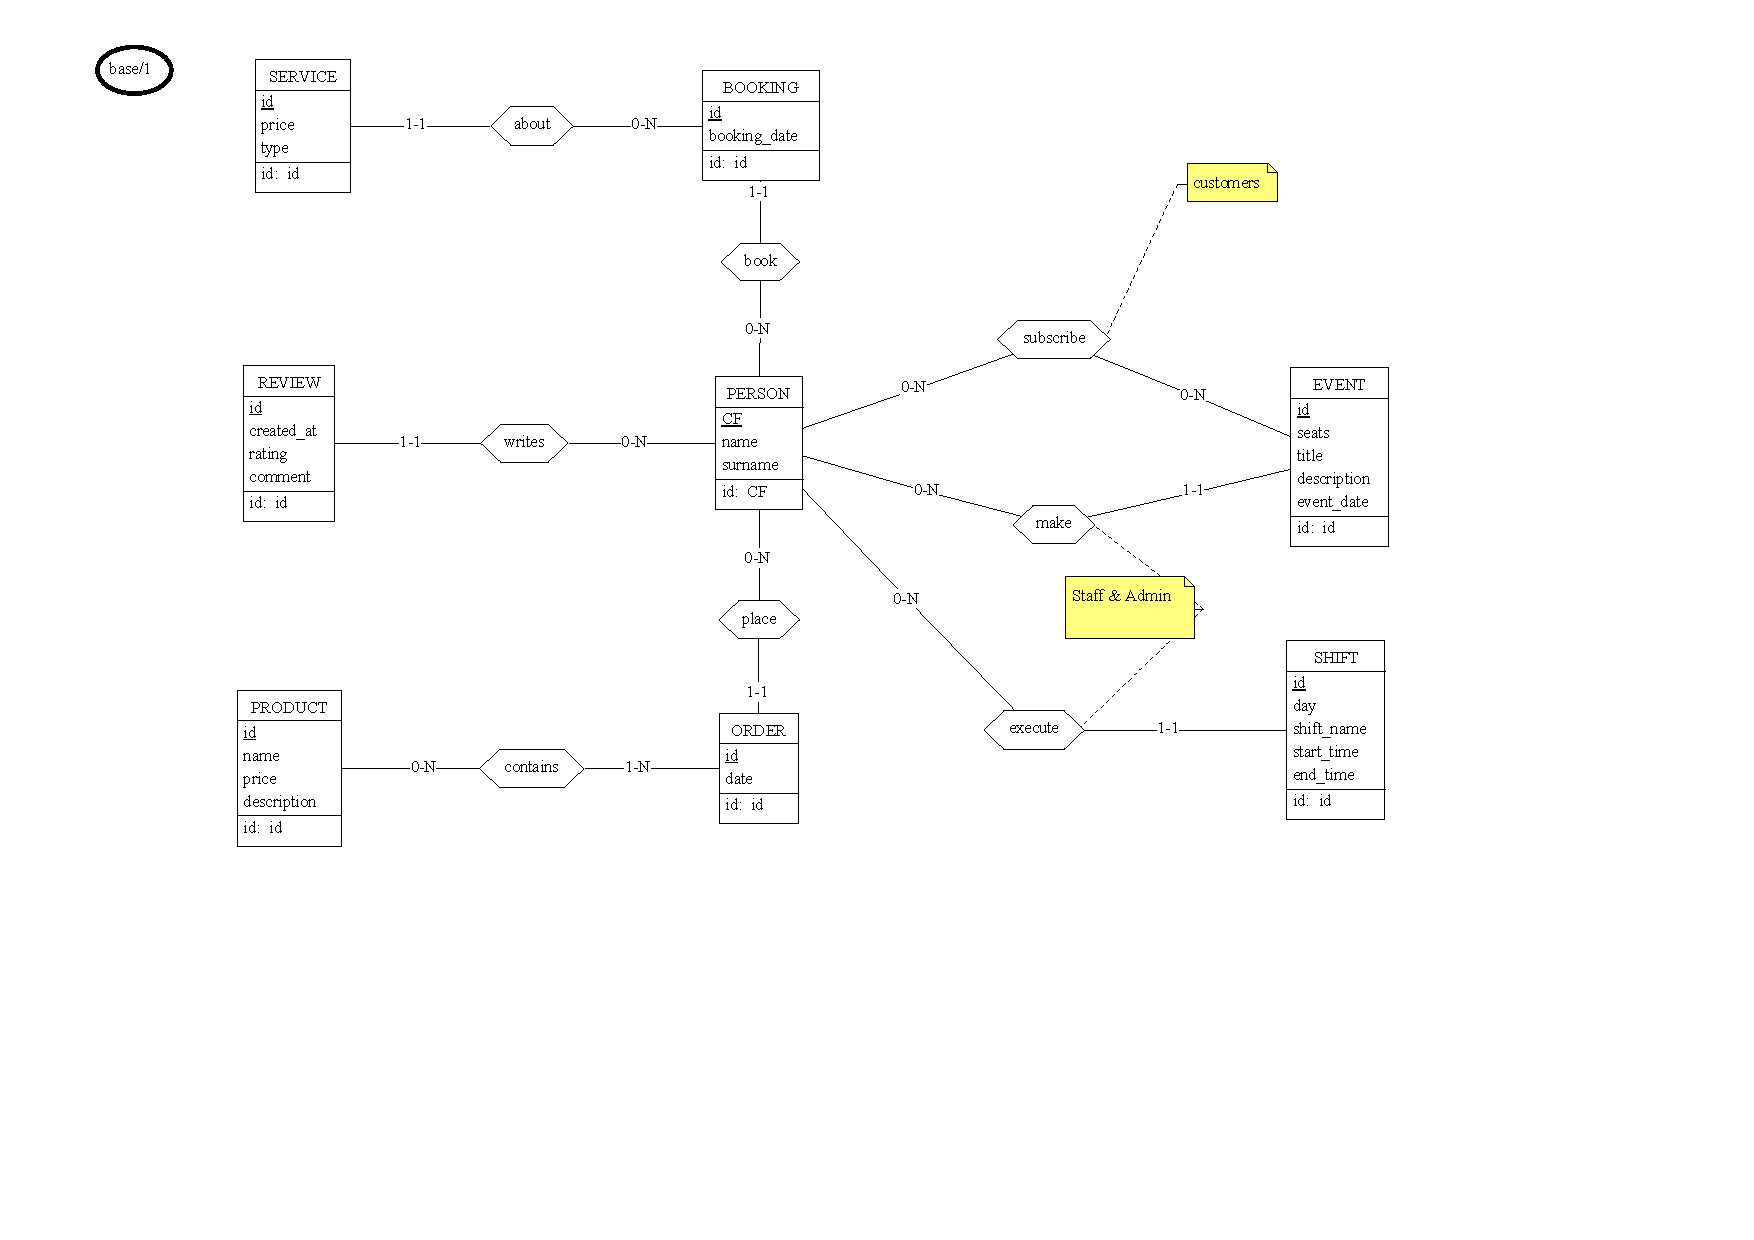
\includegraphics[width=\textwidth, trim=100pt 170pt 175pt 0pt,
  clip]{./schemas/er-base.pdf}
  \caption{Schema ER iniziale}
  \label{fig:schema-iniziale}
\end{figure}

\section{Raffinamenti proposti}
\subsection{Utente e Dipendente}
Nel modello concettuale iniziale la \textbf{Persona} raggruppava
tutte le possibili interazioni con il sistema: iscrizione, creazione
di eventi, prenotazioni, ordini e recensioni. Questo approccio,
sebbene corretto dal punto di vista logico, risultava poco chiaro
perché attribuiva a un'unica entità responsabilità molto eterogenee.

\vspace{\baselineskip}
Per migliorare la rappresentazione è stato introdotto un raffinamento
mediante generalizzazione/specializzazione: la superclasse
\textbf{Persona} è stata mantenuta per raccogliere gli attributi
comuni (CF, nome, cognome), mentre le funzionalità specifiche sono
state assegnate ai sottotipi \textbf{Cliente} e \textbf{Dipendente}.

\vspace{\baselineskip}
In questo modo i clienti gestiscono attività come acquisti,
recensioni, ordini e iscrizioni agli eventi, mentre i dipendenti si
occupano della creazione degli eventi e della gestione dei servizi.
Tale raffinamento migliora la chiarezza semantica del modello, riduce
le ambiguità e riflette meglio la separazione dei ruoli reali
all'interno del dominio applicativo.

\vspace{\baselineskip}
Il raffinamento mette in evidenza anche le dipendenze temporali (come
  la gestione dei turni \textbf{Shift} o la cronologia del personale
\textbf{Employee History}) e garantisce che ogni operazione rispetti
vincoli di consistenza e cardinalità, rendendo il modello complessivo
coerente, sicuro e facilmente estendibile.

\begin{figure}[H]
  \centering
  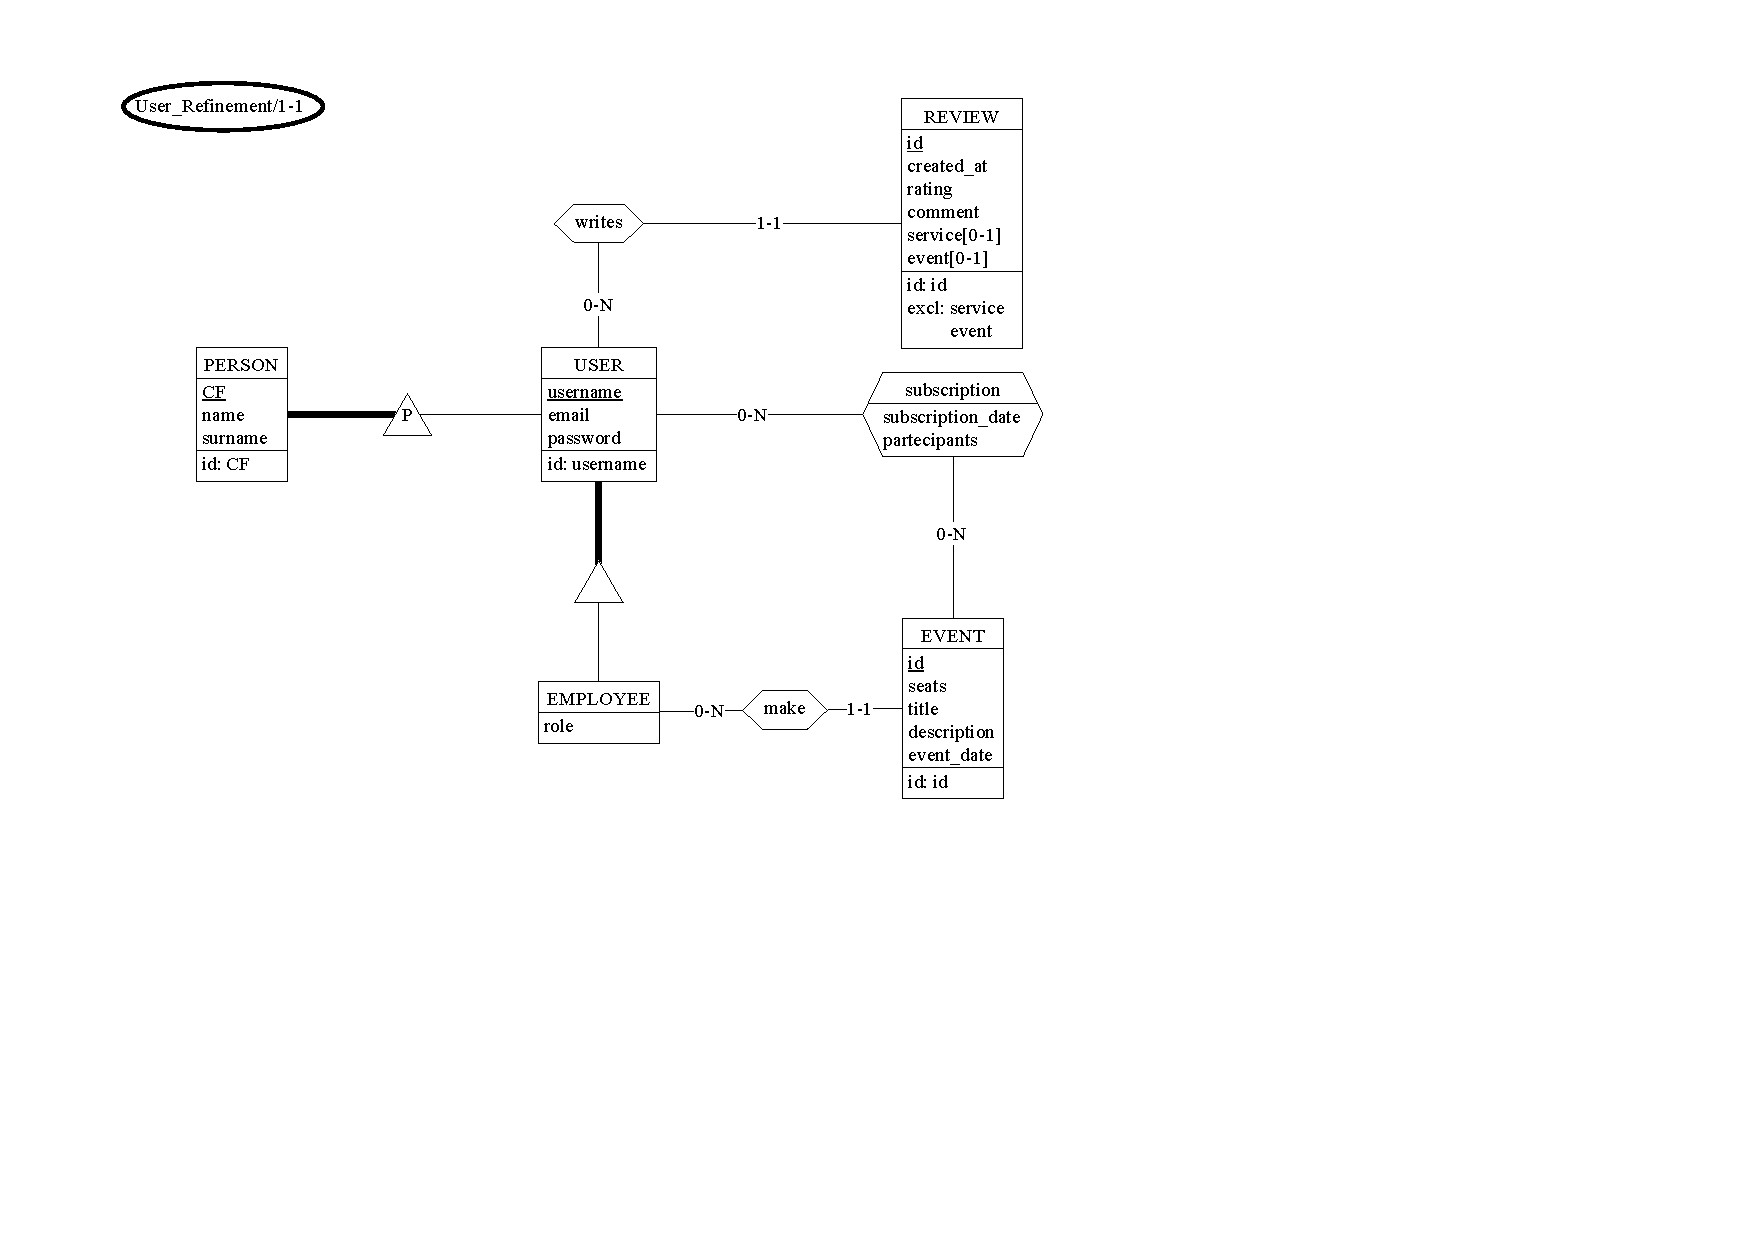
\includegraphics[width=\textwidth, trim=0 200pt 275pt 0,
  clip]{./schemas/refinements/user.pdf}
  \caption{Raffinamento utente e dipendente}
  \label{fig:raffinamento-utente}
\end{figure}

\newpage
\subsection{Prenotazione Servizi}
Nel modello iniziale i diversi tipi di servizi potevano essere
rappresentati come entità distinte, con il rischio però di ridondanza
e frammentazione dei dati.

\vspace{\baselineskip}
Con il raffinamento si è introdotta una \textbf{generalizzazione}: è
stata creata la superclasse \textbf{Servizio}, che raccoglie gli
attributi comuni (id, price, type), mentre ciascuna tipologia
specifica di servizio (Camera e Ristorante) è modellata come sottoclasse.

\vspace{\baselineskip}
Inoltre, è stato introdotto il legame con l'entità
\textbf{Prenotazione}, che consente di registrare le informazioni su
data di inizio e fine e di associare ogni prenotazione a uno o più
servizi specifici tramite la relazione con \textbf{Dettagli
Prenotazione}. Questo raffinamento permette di gestire correttamente
scenari in cui un utente prenota più servizi differenti nello stesso
arco temporale.

\begin{figure}[H]
  \centering
  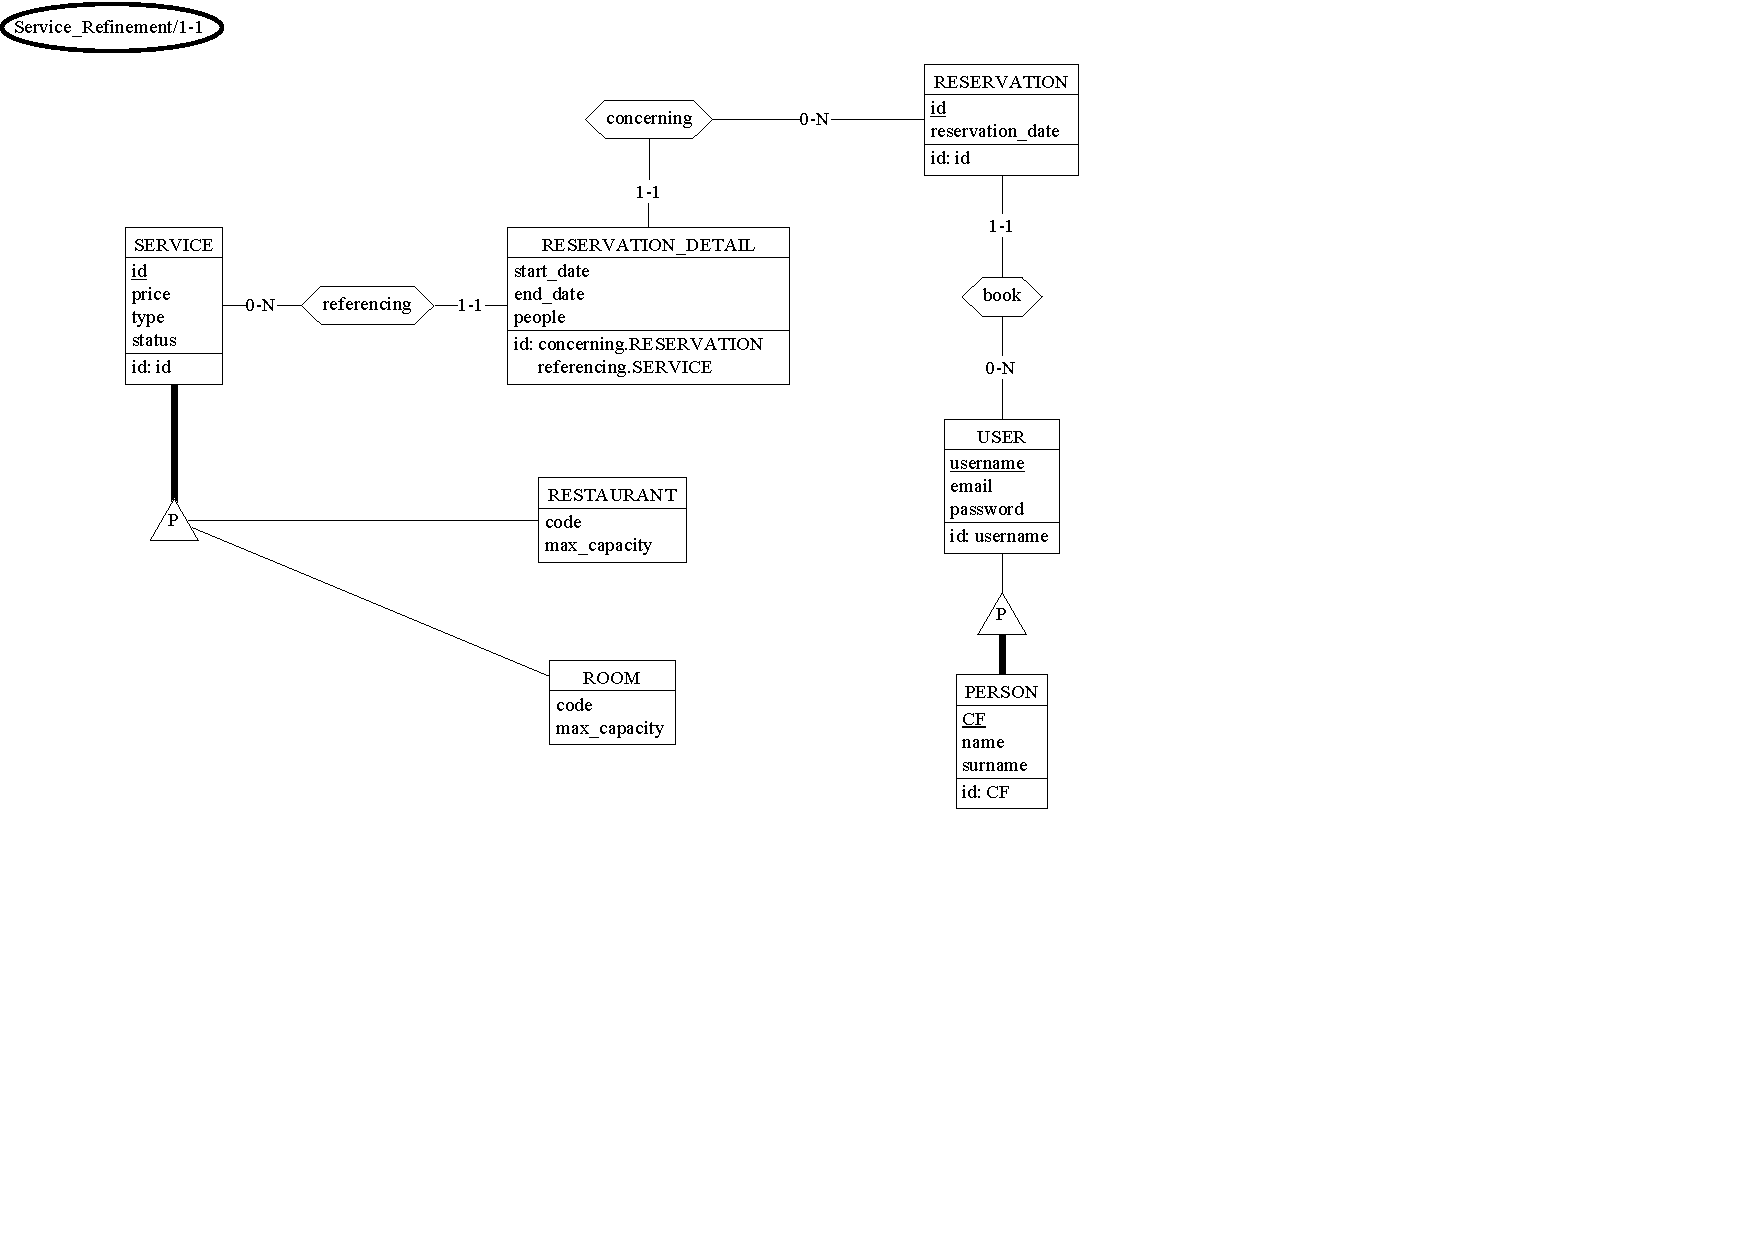
\includegraphics[width=\textwidth, trim=0 200pt 300pt 0,
  clip]{./schemas/refinements/service.pdf}
  \caption{Raffinamento prenotazione e servizi}
  \label{fig:raffinamento-servizi-prenotazione}
\end{figure}

\newpage
\subsection{Prodotti e ordini}
Nel modello concettuale iniziale, la gestione degli ordini e dei
prodotti risultava poco dettagliata: un ordine era semplicemente
collegato a uno o più prodotti, senza possibilità di specificare
informazioni aggiuntive come quantità o prezzo unitario.

\vspace{\baselineskip}
Con il raffinamento, è stata introdotta l'entità \textbf{Dettaglio
Ordine}, che funge da associazione tra \textbf{Ordine} e
\textbf{Prodotto}. Ogni dettaglio ordine consente di memorizzare, per
ciascun prodotto incluso in un ordine, la quantità acquistata e il
prezzo applicato. Questo permette di rappresentare in modo accurato
scenari reali come ordini multiprodotto, applicazione di sconti o
variazioni di prezzo nel tempo.

\vspace{\baselineskip}
Inoltre, viene mantenuta la generalizzazione tra \textbf{Persona} e
\textbf{Utente}, già introdotta nei raffinamenti precedenti, per
distinguere i dati anagrafici comuni da quelli specifici per
l'accesso al sistema e la gestione degli ordini. Questo approccio
migliora la flessibilità e la chiarezza del modello, consentendo una
gestione più efficace delle informazioni relative agli acquisti.

\begin{figure}[H]
  \centering
  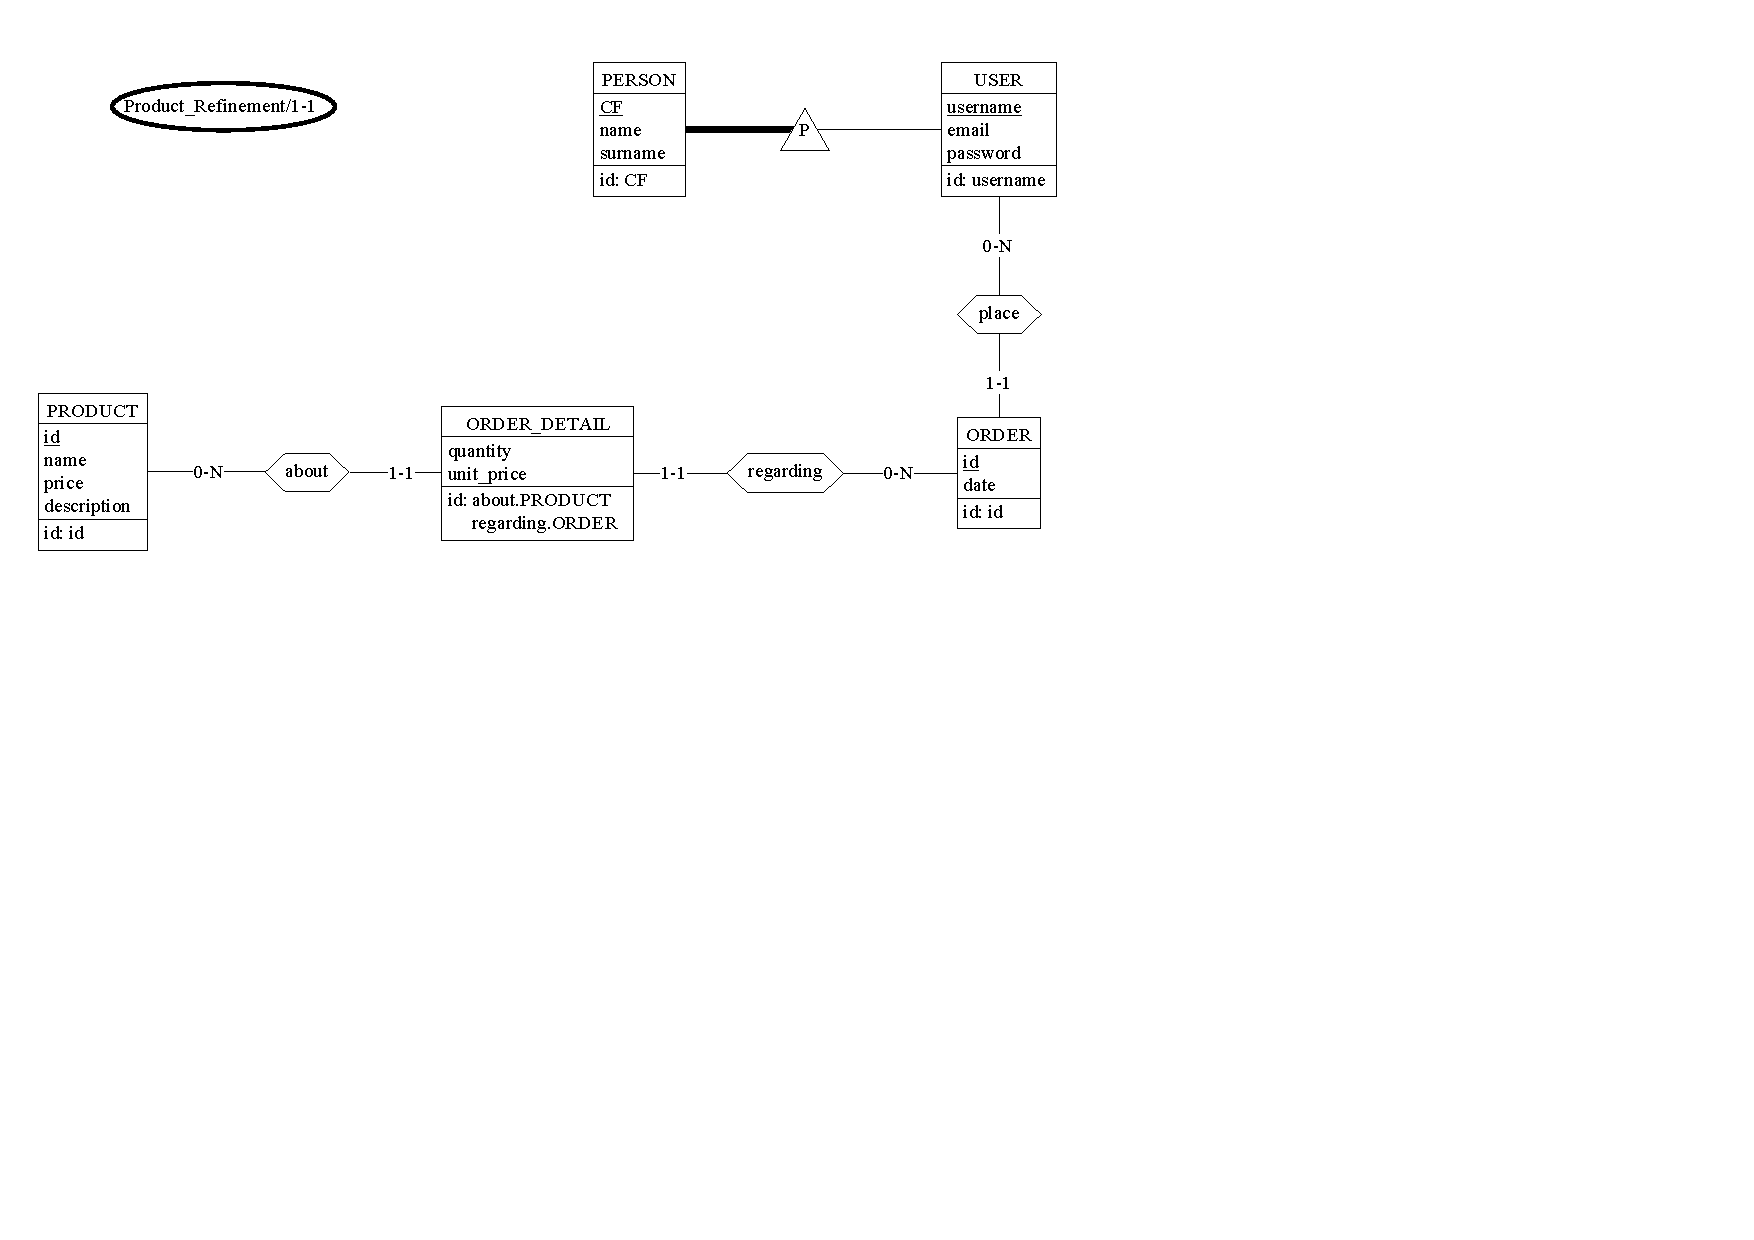
\includegraphics[width=\textwidth, trim=0 300pt 325pt 0,
  clip]{./schemas/refinements/product.pdf}
  \caption{Raffinamento prodotti e ordini}
  \label{fig:raffinamento-prodotto-ordini}
\end{figure}

\newpage
\section{Schema concettuale finale}
Qui di seguito, è presente lo schema concettuale finale con tutti i
raffinamenti.

\begin{figure}[H]
  \centering
  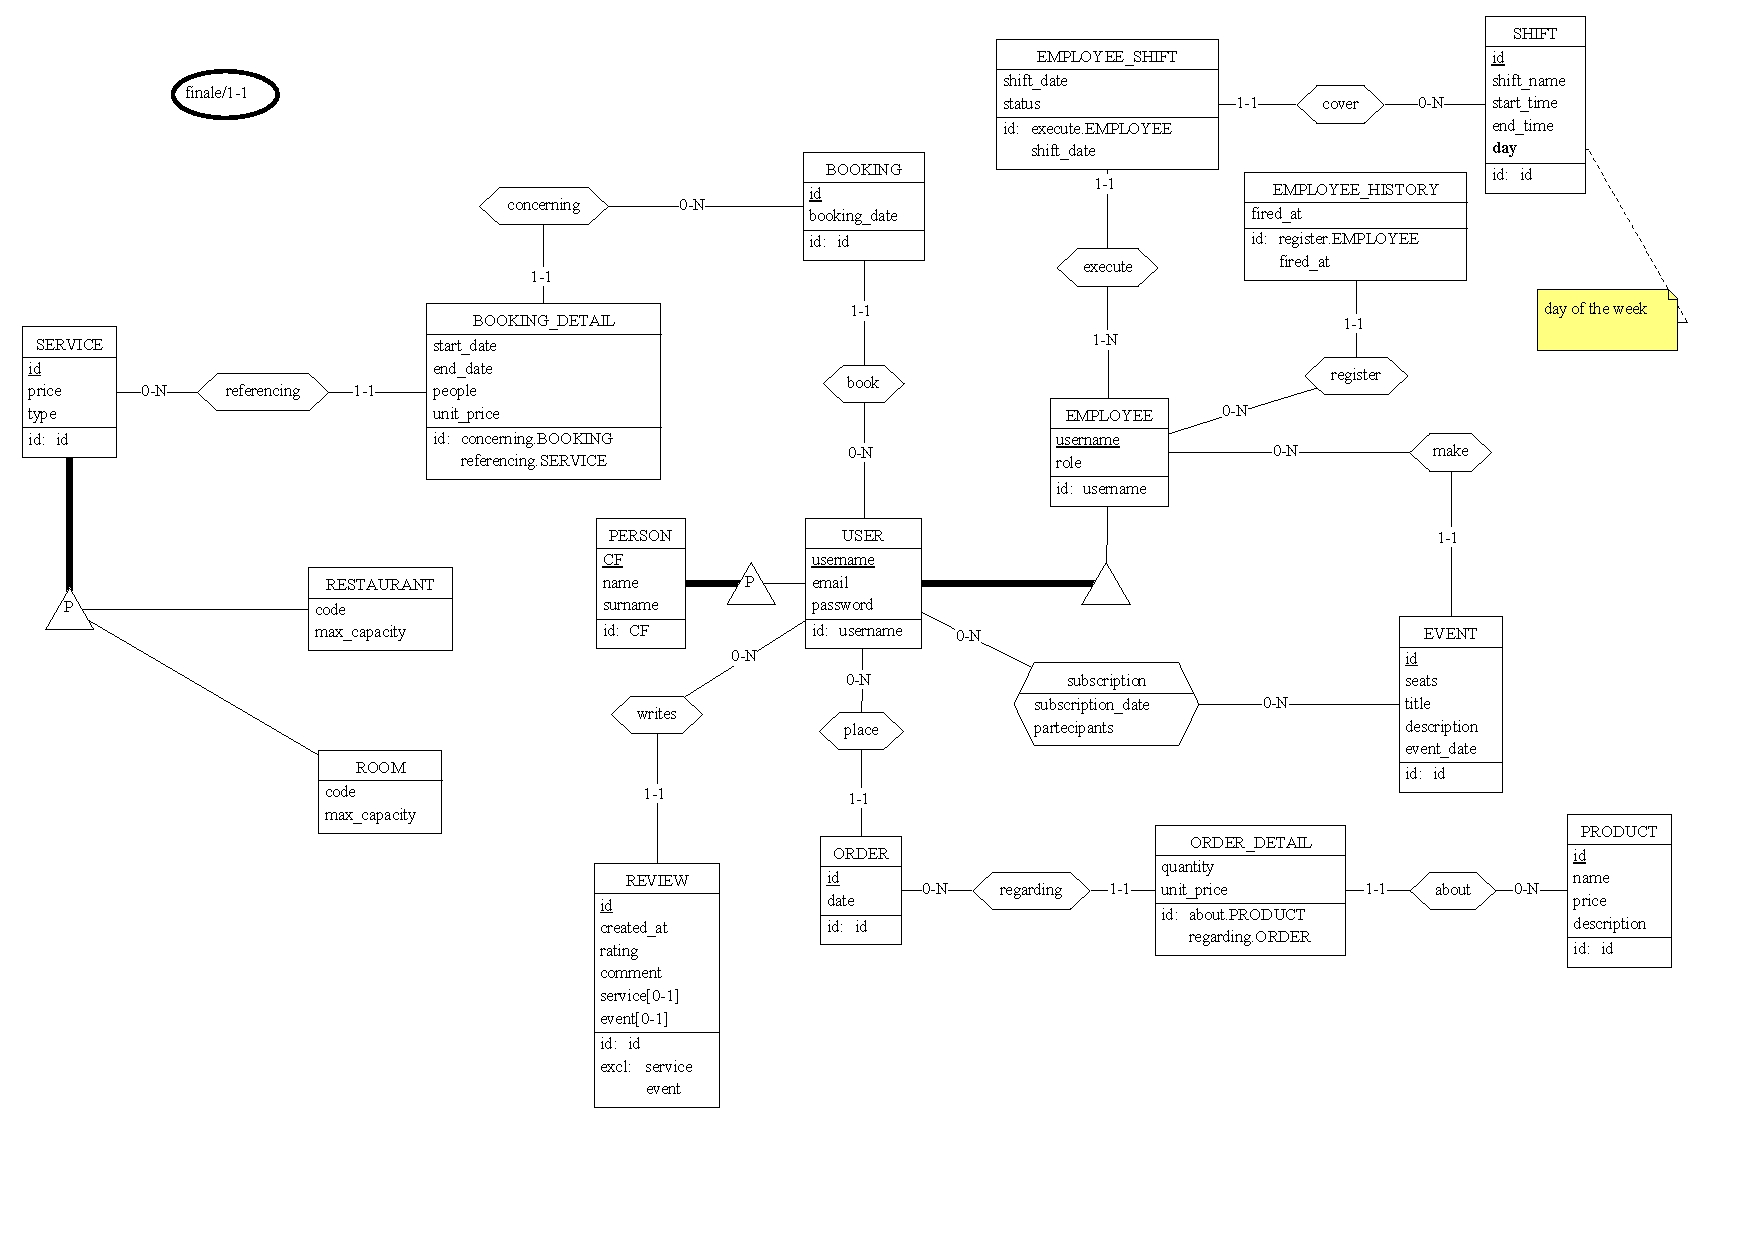
\includegraphics[width=\textwidth, trim=0 0 0
  0]{./schemas/er-final.pdf}
  \caption{Schema ER, schema concettuale finale}
  \label{fig:schema-finale}
\end{figure}

\newpage
\chapter{Progettazione Logica}
Questa sezione riassume la progettazione logica del database, con
stima dei volumi di dati e crescita attesa per ogni entità.

\section{Stima del volume di dati }
La Tabella~\ref{tab:volume-dati} riassume i volumi stimati per
ciascuna tabella e associazione, riferiti a un periodo di un anno.

\begin{table}[H]
  \centering
  \begin{tabularx}{\textwidth}{|X|c|c|}
    \hline
    \rowcolor{gray!15}
    \textbf{Tabella} & \textbf{Volume stimato} & \textbf{E/R} \\
    \hline
    \texttt{ORDER}               & 12\,000  & E \\
    \texttt{BOOKING}             & 6\,000   & E \\
    \texttt{PERSON}              & 5\,000   & E \\
    \texttt{USER}                & 4\,000   & E \\
    \texttt{REVIEW}              & 2\,500   & E \\
    \texttt{PRODUCT}             & 600      & E \\
    \texttt{EVENT}               & 200      & E \\
    \texttt{SERVICE}             & 50       & E \\
    \texttt{EMPLOYEE}            & 60       & E \\
    \texttt{ROOM}                & 22       & E \\
    \texttt{SHIFT}               & 365      & E \\
    \texttt{RESTAURANT}          & 20       & E \\
    \texttt{ORDER\_DETAIL}       & 36\,000  & E \\
    \texttt{BOOKING\_DETAIL}     & 6\,000   & E \\
    \texttt{EMPLOYEE\_SHIFT}     & 15\,000  & E \\
    \texttt{EMPLOYEE\_HISTORY}   & 100      & E \\
    \hline
    \texttt{EVENT\_SUBSCRIPTION}  & 2\,000   & R \\
    \texttt{WRITES}              & 2\,500   & R \\
    \texttt{REGISTER}            & 3\,000   & R \\
    \texttt{MAKE}                & 6\,000   & R \\
    \texttt{COVER}               & 15\,000  & R \\
    \texttt{EXECUTE}             & 15\,000  & R \\
    \texttt{CONCERNING}          & 10\,000  & R \\
    \texttt{REFERENCING}         & 10\,000  & R \\
    \texttt{ABOUT}               & 36\,000  & R \\
    \texttt{REGARDING}           & 36\,000  & R \\
    \hline
  \end{tabularx}
  \label{tab:volume-dati}
\end{table}

\section{Descrizione operazioni}
La Tabella~\ref{tab:operazioni-settimanali} mostra le principali
operazioni che gli utenti possono svolgere nel sistema, come
statistiche, prenotazioni, ordini, recensioni e autenticazione. Per
ogni operazione è indicata la frequenza settimanale stimata e il tipo
di utente che la esegue.

\begin{table}[H]
  \centering
  \small
  \renewcommand{\arraystretch}{1.12}
  \begin{tabularx}{\textwidth}{|c|>{\raggedright\arraybackslash}X|c|c|}
    \hline
    \rowcolor{gray!20}
    \textbf{\#} & \textbf{Operazione} & \textbf{Op / 7gg} &
    \textbf{Tipo Utente} \\
    \hline
    1 & \hyperref[op1]{Migliori servizi per prenotazioni} & 20 & Admin \\
    \hline
    2 & \hyperref[op2]{Migliori prodotti per quantità venduta} & 15 & Admin \\
    \hline
    3 & \hyperref[op3]{Migliori eventi per partecipanti} & 10 & Admin \\
    \hline
    4 & \hyperref[op4]{Migliori prodotti per fatturato} & 15 & Admin \\
    \hline
    5 & \hyperref[op5]{Fatturato totale} & 10 & Admin \\
    \hline
    6 & \hyperref[op6]{Statistiche generali del sistema} &
    25 & Admin / Staff \\
    \hline
    7 & \hyperref[op7]{Verifica disponibilità camere} & 50 & Tutti \\
    \hline
    8 & \hyperref[op8]{Verifica disponibilità tavoli} & 40 & Tutti \\
    \hline
    9 & \hyperref[op9]{Inserimento recensione evento} & 20
    & Cliente \\
    \hline
    10 & \hyperref[op10]{Inserimento recensione servizio} &
    30 & Cliente \\
    \hline
    11 & \hyperref[op11]{Aggiornamento recensione} & 10 & Cliente \\
    \hline
    12 & \hyperref[op12]{Update e Iscrizione utente a evento} &
    25 & Cliente \\
    \hline
    13 & \hyperref[op13]{Creazione prenotazione principale} & 100 &
    Cliente / Staff \\
    \hline
    14 & \hyperref[op14]{Prenotazione tavolo ristorante} & 80 &
    Cliente / Staff \\
    \hline
    15 & \hyperref[op15]{Prenotazione camera con controllo duplicati}
    & 70 & Cliente / Staff \\
    \hline
    16 & \hyperref[op16]{Eliminazione prenotazione servizio} & 20 &
    Cliente / Staff \\
    \hline
    17 & \hyperref[op17]{Eliminazione iscrizione evento} &
    15 & Cliente \\
    \hline
    18 & \hyperref[op18]{Eliminazione prenotazione con controllo
    temporale} & 15 & Cliente / Staff \\
    \hline
    19 & \hyperref[op19]{Verifica credenziali di login} &
    500 & Tutti \\
    \hline
    20 & \hyperref[op20]{Creazione nuovo ordine} & 60 &
    Cliente / Staff \\
    \hline
  \end{tabularx}
  \caption{Numero stimato di operazioni per settimana, con tipo di
  utente che le effettua}
  \label{tab:operazioni-settimanali}
\end{table}

\section{Analisi delle operazioni}
Di seguito viene riportata un'analisi delle principali operazioni
sul database dell'agriturismo.

Si definiscono:
\begin{itemize}
  \item $Op_{sett}$: numero di volte che l'operazione viene eseguita
    settimanalmente
  \item $C_{tot}$: costo totale dell'operazione (accessi settimanali)
  \item $A_{scr}$: numero di accessi in scrittura per operazione
    (ogni scrittura conta come \textbf{2 accessi})
  \item $A_{lett}$: numero di accessi in lettura per operazione
\end{itemize}

\newpage
\subsection*{Migliori servizi per prenotazioni} \label{op1}
\colorbox{yellow}{Identifica i servizi più prenotati distinguendo tra
ristoranti e camere.}

Mostra quali servizi (camere e ristoranti) sono
prenotati più spesso, fornendo una classifica utile per capire la
domanda e gestire meglio le risorse.

$$Op_{sett} = 20$$

\begin{table}[H]
  \centering
  \small
  \renewcommand{\arraystretch}{1.15}
  \begin{tabularx}{0.7\textwidth}{|X|c|c|c|}
    \hline
    \rowcolor{gray!20}
    \textbf{Tabella} & \textbf{Tipo} & \textbf{S/L} & \textbf{Accessi} \\
    \hline
    BOOKING\_DETAIL & R & L & 6\,000 \\
    RESTAURANT & E & L & 20 \\
    SERVICE & E & L & 25 \\
    ROOM & E & L & 22 \\
    \hline
    \rowcolor{gray!20}
    TOTALE & & & 6\,067 \\
    \hline
  \end{tabularx}
  \vspace{-1em}
\end{table}

$$\mathbf{C_{tot}} = 20 \cdot 6\,067 = \mathbf{121\,340}$$

\subsection*{Migliori prodotti per quantità venduta} \label{op2}
\colorbox{yellow}{Calcola i prodotti più venduti in base alla
quantità totale ordinata.}

Classifica i prodotti in base alla quantità totale venduta, utile per
analizzare le preferenze dei clienti e ottimizzare l'offerta.

$$Op_{sett} = 15$$

\begin{table}[H]
  \centering
  \small
  \renewcommand{\arraystretch}{1.15}
  \begin{tabularx}{0.7\textwidth}{|X|c|c|c|}
    \hline
    \rowcolor{gray!20}
    \textbf{Tabella} & \textbf{Tipo} & \textbf{S/L} & \textbf{Accessi} \\
    \hline
    ORDER\_DETAIL & R & L & 36\,000 \\
    PRODUCT & E & L & 600 \\
    \hline
    \rowcolor{gray!20}
    TOTALE & & & 36\,600 \\
    \hline
  \end{tabularx}
  \vspace{-1em}
\end{table}

$$\mathbf{C_{tot}} = 15 \cdot 36\,600 = \mathbf{549\,000}$$

\subsection*{Migliori eventi per partecipanti} \label{op3}
\colorbox{yellow}{Determina gli eventi con il maggior numero di
partecipanti totali.}

Individua gli eventi che hanno raccolto il maggior numero di
iscritti, fornendo una classifica utile per analizzare la popolarità
delle iniziative e ottimizzare la pianificazione futura.

$$Op_{sett} = 10$$

\begin{table}[H]
  \centering
  \small
  \renewcommand{\arraystretch}{1.15}
  \begin{tabularx}{0.7\textwidth}{|X|c|c|c|}
    \hline
    \rowcolor{gray!20}
    \textbf{Tabella} & \textbf{Tipo} & \textbf{S/L} & \textbf{Accessi}  \\
    \hline
    EVENT\_SUBSCRIPTION & R & L & 2\,000 \\
    EVENT & E & L & 200 \\
    \hline
    \rowcolor{gray!20}
    TOTALE & & & 2\,200 \\
    \hline
  \end{tabularx}
  \vspace{-1em}
\end{table}

$$\mathbf{C_{tot}} = 10 \cdot 2\,200 = \mathbf{22\,000}$$

\subsection*{Migliori prodotti per fatturato} \label{op4}
\colorbox{yellow}{Calcola i prodotti che generano il maggior fatturato.}

Identifica i prodotti che generano più fatturato, mostrando il totale
ricavi per ciascun articolo.

$$Op_{sett} = 15$$

\begin{table}[H]
  \centering
  \small
  \renewcommand{\arraystretch}{1.15}
  \begin{tabularx}{0.7\textwidth}{|X|c|c|c|}
    \hline
    \rowcolor{gray!20}
    \textbf{Tabella} & \textbf{Tipo} & \textbf{S/L} & \textbf{Accessi} \\
    \hline
    ORDER\_DETAIL & R & L & 36\,000 \\
    PRODUCT & E & L & 600 \\
    \hline
    \rowcolor{gray!20}
    TOTALE & & & 36\,600\\
    \hline
  \end{tabularx}
  \vspace{-1em}
\end{table}

$$\mathbf{C_{tot}} = 15 \cdot 36\,600 = \mathbf{549\,000}$$

\subsection*{Fatturato totale} \label{op5}

\colorbox{yellow}{Calcola il ricavo complessivo dalle vendite dei prodotti.}

Calcola il totale dei ricavi generati dagli ordini di prodotti, utile
per monitorare l'andamento economico.

$$Op_{sett} = 10$$

\begin{table}[H]
  \centering
  \small
  \renewcommand{\arraystretch}{1.15}
  \begin{tabularx}{0.7\textwidth}{|X|c|c|c|}
    \hline
    \rowcolor{gray!20}
    \textbf{Tabella} & \textbf{Tipo} & \textbf{S/L} & \textbf{Accessi} \\
    \hline
    ORDER\_DETAIL & E & L & 36\,000 \\
    BOOKING\_DETAIL & E & L & 6\,000 \\
    \hline
    \rowcolor{gray!20}
    TOTALE & & & 42\,000 \\
    \hline
  \end{tabularx}
  \vspace{-1em}
\end{table}

$$\mathbf{C_{tot}} = 10 \cdot 42\,000 = \mathbf{420\,000}$$

\subsection*{Statistiche generali del sistema} \label{op6}
\colorbox{yellow}{Calcola le principali metriche aggregate del sistema.}

Mostra i numeri principali del sistema: utenti, dipendenti, ordini,
dettagli ordine e prenotazioni. Serve per avere una visione rapida e
generale della piattaforma.

$$Op_{sett} = 25$$

\begin{table}[H]
  \centering
  \small
  \renewcommand{\arraystretch}{1.15}
  \begin{tabularx}{0.7\textwidth}{|X|c|c|c|}
    \hline
    \rowcolor{gray!20}
    \textbf{Tabella} & \textbf{Tipo} & \textbf{S/L} & \textbf{Accessi} \\
    \hline
    ORDER\_DETAIL & E & L & 36\,000 \\
    ORDER & E & L & 12\,000\\
    BOOKING & E & L & 6\,000 \\
    USER & E & L & 4\,000 \\
    EMPLOYEE & E & L & 60 \\
    \hline
    \rowcolor{gray!20}
    TOTALE & & & 58\,060 \\
    \hline
  \end{tabularx}
  \vspace{-1em}
\end{table}

$$\mathbf{C_{tot}} = 25 \cdot 58\,060 = \mathbf{1\,451\,500}$$

\subsection*{Verifica disponibilità camere} \label{op7}
\colorbox{yellow}{Verifica la disponibilità delle camere in un dato periodo.}

Verifica quali camere sono libere per un intervallo di date e numero
di persone, evitando sovrapposizioni con prenotazioni esistenti.

$$Op_{sett} = 50$$

\begin{table}[H]
  \centering
  \small
  \renewcommand{\arraystretch}{1.15}
  \begin{tabularx}{0.7\textwidth}{|X|c|c|c|}
    \hline
    \rowcolor{gray!20}
    \textbf{Nome} & \textbf{Tipo} & \textbf{S/L} &\textbf{Accessi} \\
    \hline
    BOOKING\_DETAIL & E & L & 6\,000 \\
    ROOM & E & L & 22 \\
    SERVICE & E & L & 25 \\
    \hline
    \rowcolor{gray!20}
    TOTALE & & & 6\,047 \\
    \hline
  \end{tabularx}
  \vspace{-1em}
\end{table}

$$\mathbf{C_{tot}} = 50 \cdot 6\,047 = \mathbf{302\,350}$$

\subsection*{Verifica disponibilità tavoli} \label{op8}
\colorbox{yellow}{Verifica la disponibilità dei tavoli al ristorante.}

Controlla i tavoli liberi in un intervallo di data/ora, evitando
sovrapposizioni con prenotazioni esistenti.

$$Op_{sett} = 40$$

\begin{table}[H]
  \centering
  \small
  \renewcommand{\arraystretch}{1.15}
  \begin{tabularx}{0.7\textwidth}{|X|c|c|c|}
    \hline
    \rowcolor{gray!20}
    \textbf{Tabella} & \textbf{Tipo} & \textbf{S/L} & \textbf{Accessi} \\
    \hline
    BOOKING\_DETAIL & E & L & 6000 \\
    RESTAURANT & E & L & 20 \\
    SERVICE & E & L & 20 \\
    \hline
    \rowcolor{gray!20}
    TOTALE & & & 6\,040 \\
    \hline
  \end{tabularx}
  \vspace{-1em}
\end{table}

$$\mathbf{C_{tot}} = 40 \cdot 6\,040 = \mathbf{241\,600}$$

\subsection*{Inserimento recensione evento} \label{op9}
\colorbox{yellow}{Inserisce una recensione per un evento.}

Registra una recensione associata a un evento a cui l'utente ha partecipato.

$$Op_{sett} = 20$$

\begin{table}[H]
  \centering
  \small
  \renewcommand{\arraystretch}{1.15}
  \begin{tabularx}{0.7\textwidth}{|X|c|c|c|}
    \hline
    \rowcolor{gray!20}
    \textbf{Tabella} & \textbf{Tipo} & \textbf{Numero accessi} & \textbf{S/L} \\
    \hline
    EVENT\_SUBSCRIPTION & R & 1 & L \\
    REVIEW & E & 1 & S \\
    EVENT & E & 1 & L \\
    \hline
    \rowcolor{gray!20}
    TOTALE & & & 3\\
    \hline
  \end{tabularx}
  \vspace{-1em}
\end{table}

$$\mathbf{C_{tot}} = 20 \cdot (2 + 2 \cdot 1) = \mathbf{60}$$

\subsection*{Inserimento recensione servizio} \label{op10}
\colorbox{yellow}{Inserisce una recensione per un servizio.}

Registra una recensione su un servizio (camera/ristorante) legato a
una prenotazione.

$$Op_{sett} = 30$$

\begin{table}[H]
  \centering
  \small
  \renewcommand{\arraystretch}{1.15}
  \begin{tabularx}{0.7\textwidth}{|X|c|c|c|}
    \hline
    \rowcolor{gray!20}
    \textbf{Tabella} & \textbf{Tipo} & \textbf{S/L} & \textbf{Accessi} \\
    \hline
    BOOKING\_DETAIL & R & L & 1\\
    SERVICE & E & L & 1 \\
    BOOKING & E & L & 1 \\
    REVIEW & E & S & 1 \\
    \hline
    \rowcolor{gray!20}
    TOTALE & & & 4 \\
    \hline
  \end{tabularx}
  \vspace{-1em}
\end{table}

$$\mathbf{C_{tot}} = 30 \cdot (3 + 2 \cdot 1) = \mathbf{150}$$

\subsection*{Aggiornamento recensione} \label{op11}
\colorbox{yellow}{Aggiorna una recensione esistente.}

Modifica il contenuto di una recensione precedentemente inserita dall'utente.

$$Op_{sett} = 10$$

\begin{table}[H]
  \centering
  \small
  \renewcommand{\arraystretch}{1.15}
  \begin{tabularx}{0.7\textwidth}{|X|c|c|c|}
    \hline
    \rowcolor{gray!20}
    \textbf{Tabella} & \textbf{Tipo} & \textbf{S/L} & \textbf{Accessi} \\
    \hline
    REVIEW & E & L & 1 \\
    REVIEW & E & S & 1 \\
    \hline
    \rowcolor{gray!20}
    TOTALE & & & 2 \\
    \hline
  \end{tabularx}
  \vspace{-1em}
\end{table}

$$\mathbf{C_{tot}} = 10 \cdot (1 + 2 \cdot 1) = \mathbf{30}$$

\subsection*{Update e Iscrizione utente a evento} \label{op12}
\colorbox{yellow}{Iscrive un utente a un evento o aggiorna l'iscrizione.}

Gestisce la creazione o l'aggiornamento dell'iscrizione di un utente
a un evento.

$$Op_{sett} = 25$$

\begin{table}[H]
  \centering
  \small
  \renewcommand{\arraystretch}{1.15}
  \begin{tabularx}{0.7\textwidth}{|X|c|c|c|}
    \hline
    \rowcolor{gray!20}
    \textbf{Tabella} & \textbf{Tipo} & \textbf{S/L} & \textbf{Accessi} \\
    \hline
    EVENT\_SUBSCRIPTION & R & S & 1 \\
    EVENT & E & L & 1 \\
    USER & E & L & 1 \\
    \hline
    \rowcolor{gray!20}
    TOTALE & & & 3 \\
    \hline
  \end{tabularx}
  \vspace{-1em}
\end{table}

$$\mathbf{C_{tot}} = 25 \cdot (2 + 2 \cdot 1) = \mathbf{100}$$

\subsection*{Creazione prenotazione principale} \label{op13}
\colorbox{yellow}{Crea il record principale di una prenotazione.}

Avvia una prenotazione registrando l'intestazione collegata all'utente.

$$Op_{sett} = 100$$

\begin{table}[H]
  \centering
  \small
  \renewcommand{\arraystretch}{1.15}
  \begin{tabularx}{0.7\textwidth}{|X|c|c|c|}
    \hline
    \rowcolor{gray!20}
    \textbf{Tabella} & \textbf{Tipo} & \textbf{S/L} & \textbf{Accessi} \\
    \hline
    BOOKING & E & S & 1 \\
    USER & E & L & 1 \\
    \hline
    \rowcolor{gray!20}
    TOTALE & & & 2 \\
    \hline
  \end{tabularx}
  \vspace{-1em}
\end{table}

$$\mathbf{C_{tot}} = 100 \cdot (1 + 2 \cdot 1) = \mathbf{300}$$

\subsection*{Prenotazione tavolo ristorante} \label{op14}
\colorbox{yellow}{Registra la prenotazione di un tavolo al ristorante.}

Associa il servizio ristorante ai dettagli della prenotazione,
evitando duplicazioni.

$$Op_{sett} = 80$$

\begin{table}[H]
  \centering
  \small
  \renewcommand{\arraystretch}{1.15}
  \begin{tabularx}{0.7\textwidth}{|X|c|c|c|}
    \hline
    \rowcolor{gray!20}
    \textbf{Tabella} & \textbf{Tipo} & \textbf{S/L} & \textbf{Accessi} \\
    \hline
    BOOKING\_DETAIL & R & S & 1 \\
    SERVICE & E & L & 1 \\
    RESTAURANT & E & L & 1 \\
    \hline
    \rowcolor{gray!20}
    TOTALE & & & 3 \\
    \hline
  \end{tabularx}
  \vspace{-1em}
\end{table}

$$\mathbf{C_{tot}} = 80 \cdot (2 + 2 \cdot 1) = \mathbf{320}$$

\subsection*{Prenotazione camera con controllo duplicati} \label{op15}
\colorbox{yellow}{Prenota una camera con controlli anti-duplicati.}

Registra una prenotazione camera controllando che non esistano già
prenotazioni sovrapposte per lo stesso utente e periodo.

$$Op_{sett} = 70$$

\begin{table}[H]
  \centering
  \small
  \renewcommand{\arraystretch}{1.15}
  \begin{tabularx}{0.7\textwidth}{|X|c|c|c|}
    \hline
    \rowcolor{gray!20}
    \textbf{Tabella} & \textbf{Tipo} & \textbf{S/L} & \textbf{Accessi} \\
    \hline
    BOOKING\_DETAIL & R & S & 1 \\
    BOOKING & E & L & 1 \\
    SERVICE & E & L & 1 \\
    ROOM & E & L & 1 \\
    \hline
    \rowcolor{gray!20}
    TOTALE & & & 4 \\
    \hline
  \end{tabularx}
  \vspace{-1em}
\end{table}

$$\mathbf{C_{tot}} = 70 \cdot (3 + 2 \cdot 1) = \mathbf{350}$$

\subsection*{Eliminazione prenotazione servizio} \label{op16}
\colorbox{yellow}{Elimina una prenotazione di servizio.}

Rimuove un dettaglio di prenotazione e aggiorna lo stato della
prenotazione principale.

$$Op_{sett} = 20$$

\begin{table}[H]
  \centering
  \small
  \renewcommand{\arraystretch}{1.15}
  \begin{tabularx}{0.7\textwidth}{|X|c|c|c|}
    \hline
    \rowcolor{gray!20}
    \textbf{Tabella} & \textbf{Tipo} & \textbf{S/L} & \textbf{Accessi} \\
    \hline
    BOOKING\_DETAIL & R & L & 2 \\
    BOOKING\_DETAIL & R & S & 2 \\
    BOOKING & E & L & 1 \\
    BOOKING & E & S & 1 \\
    \hline
    \rowcolor{gray!20}
    TOTALE & & & 4 \\
    \hline
  \end{tabularx}
  \vspace{-1em}
\end{table}

$$\mathbf{C_{tot}} = 20 \cdot (3 + 2 \cdot 3) = \mathbf{180}$$

\subsection*{Eliminazione iscrizione evento} \label{op17}
\colorbox{yellow}{Elimina l'iscrizione a un evento.}

Cancella la sottoscrizione a un evento mantenendo la coerenza dei
posti disponibili.

$$Op_{sett} = 15$$

\begin{table}[H]
  \centering
  \small
  \renewcommand{\arraystretch}{1.15}
  \begin{tabularx}{0.7\textwidth}{|X|c|c|c|}
    \hline
    \rowcolor{gray!20}
    \textbf{Tabella} & \textbf{Tipo} & \textbf{S/L} & \textbf{Accessi} \\
    \hline
    EVENT\_SUBSCRIPTION & R & L & 1 \\
    EVENT\_SUBSCRIPTION & R & S & 1 \\
    EVENT & E & 1 & L \\
    \hline
    \rowcolor{gray!20}
    TOTALE & & & 3 \\
    \hline
  \end{tabularx}
  \vspace{-1em}
\end{table}

$$\mathbf{C_{tot}} = 15 \cdot (2 + 2 \cdot 1) = \mathbf{60}$$

\subsection*{Eliminazione prenotazione con controllo temporale} \label{op18}
\colorbox{yellow}{Elimina una prenotazione non ancora iniziata.}

Consente l'eliminazione solo se la prenotazione non è già iniziata
alla data corrente.

$$Op_{sett} = 15$$

\begin{table}[H]
  \centering
  \small
  \renewcommand{\arraystretch}{1.15}
  \begin{tabularx}{0.7\textwidth}{|X|c|c|c|}
    \hline
    \rowcolor{gray!20}
    \textbf{Tabella} & \textbf{Tipo} & \textbf{S/L} & \textbf{Accessi} \\
    \hline
    BOOKING\_DETAIL & R & L & 2 \\
    BOOKING & E & L & 1 \\
    BOOKING & E & S & 1  \\
    \hline
    \rowcolor{gray!20}
    TOTALE & & & 3 \\
    \hline
  \end{tabularx}
  \vspace{-1em}
\end{table}

$$\mathbf{C_{tot}} = 15 \cdot (3 + 2 \cdot 3) = \mathbf{135}$$

\subsection*{Verifica credenziali di login} \label{op19}
\colorbox{yellow}{Verifica username e password per il login.}

Controlla le credenziali confrontando utente, persona e vista del
personale attivo.

$$Op_{sett} = 500$$

\begin{table}[H]
  \centering
  \small
  \renewcommand{\arraystretch}{1.15}
  \begin{tabularx}{0.7\textwidth}{|X|c|c|c|}
    \hline
    \rowcolor{gray!20}
    \textbf{Tabella} & \textbf{Tipo} & \textbf{S/L} & \textbf{Accessi} \\
    \hline
    USER   & E & L & 1 \\
    EMPLOYEE & E & L & 1 \\
    EMPLOYEE\_HISTORY & E & L & 1 \\
    \hline
    \rowcolor{gray!20}
    TOTALE & & & 3 \\
    \hline
  \end{tabularx}
  \vspace{-1em}
\end{table}

$$\mathbf{C_{tot}} = 500 \cdot 3 = \mathbf{1\,500}$$

\subsection*{Creazione nuovo ordine} \label{op20}
\colorbox{yellow}{Crea un nuovo ordine con i relativi dettagli.}

Inserisce l'ordine principale e i dettagli riga collegati ai prodotti
selezionati.

$$Op_{sett} = 60$$

\begin{table}[H]
  \centering
  \small
  \renewcommand{\arraystretch}{1.15}
  \begin{tabularx}{0.7\textwidth}{|X|c|c|c|}
    \hline
    \rowcolor{gray!20}
    \textbf{Nome} & \textbf{Tipo} & \textbf{S/L} & \textbf{Accessi} \\
    \hline
    ORDER\_DETAIL & R & S & 3 \\
    ORDERS & E & S & 1 \\
    USER & E & L & 1 \\
    PRODUCT & E & L & 3 \\
    \hline
    \rowcolor{gray!20}
    TOTALE & & & 8 \\
    \hline
  \end{tabularx}
  \vspace{-1em}
\end{table}

$$\mathbf{C_{tot}} = 60 \cdot (5 + 2 \cdot 4) = \mathbf{780}$$

\newpage
\section{Riepilogo operazioni}
Il riepilogo seguente mostra i costi settimanali stimati per ciascuna
operazione principale del sistema, suddivisi per tipologia di utente.
La tabella consente di valutare l'impatto delle diverse funzionalità
sul carico del database e di identificare le aree più critiche dal
punto di vista delle prestazioni.

\begin{table}[H]
  \centering
  \small
  \renewcommand{\arraystretch}{1.2}
  \begin{tabularx}{\textwidth}{|>{\raggedright\arraybackslash}X|c|c|}
    \hline
    \rowcolor{gray!20}
    \textbf{Operazione} & \textbf{Costo totale/7gg} & \textbf{Tipo Utente} \\
    \hline
    Migliori servizi per prenotazioni & 121\,340 & Admin \\
    \hline
    Migliori prodotti per quantità venduta & 549\,000 & Admin \\
    \hline
    Migliori eventi per partecipanti & 22\,000 & Admin \\
    \hline
    Migliori prodotti per fatturato & 549\,000 & Admin \\
    \hline
    Fatturato totale & 420\,000 & Admin \\
    \hline
    Statistiche generali del sistema & 1\,451\,500 & Admin / Staff \\
    \hline
    Verifica disponibilità camere & 302\,350 & Tutti \\
    \hline
    Verifica disponibilità tavoli & 241\,600 & Tutti \\
    \hline
    Inserimento recensione evento & 60 & Cliente \\
    \hline
    Inserimento recensione servizio & 150 & Cliente \\
    \hline
    Aggiornamento recensione & 30 & Cliente \\
    \hline
    Update e Iscrizione utente a evento & 100 & Cliente \\
    \hline
    Creazione prenotazione principale & 300 & Cliente / Staff \\
    \hline
    Prenotazione tavolo ristorante & 320 & Cliente / Staff \\
    \hline
    Prenotazione camera con controllo duplicati & 350 & Cliente / Staff \\
    \hline
    Eliminazione prenotazione servizio & 180 & Cliente / Staff \\
    \hline
    Eliminazione iscrizione evento & 60 & Cliente \\
    \hline
    Eliminazione prenotazione con controllo temporale & 135 & Cliente / Staff \\
    \hline
    Verifica credenziali di login & 1\,500 & Tutti \\
    \hline
    Creazione nuovo ordine & 780 & Cliente / Staff \\
    \hline
    \rowcolor{gray!20}
    \textbf{TOTALE} & \textbf{3\,660\,575} & \\
    \hline
  \end{tabularx}
  \caption{Riepilogo delle operazioni con costi settimanali e tipi di utente}
  \label{tab:riepilogo-operazioni}
\end{table}

\newpage
\section{Raffinamento dello schema}
In questa sezione vengono descritti i principali raffinamenti dello
schema ER per la traduzione nel modello relazionale: rimozione
attributi multivalore, gestione delle gerarchie, reificazione delle
associazioni molti-a-molti e scelta degli identificatori.

\subsection{Rimozione gerarchie}
Nel nostro schema ER sono presenti alcune gerarchie
(generalizzazioni) che richiedono una traduzione appropriata nel
modello relazionale. Di seguito analizziamo ciascun caso specifico e
le relative scelte implementative.

\subsubsection{Gerarchia di Servizio}
La gerarchia tra \texttt{Service}, \texttt{Room} e
\texttt{Restaurant} è totale ed esclusiva: ogni servizio è
rappresentato da una sola sottoclasse. Gli attributi comuni risiedono
in \texttt{Service}, mentre le caratteristiche specifiche sono
gestite nelle tabelle specializzate collegate tramite chiave esterna.
Il campo \texttt{type} consente di distinguere rapidamente la
tipologia e il modello resta espandibile per nuovi servizi.

\subsubsection{Gerarchia di Persona}
La gerarchia tra \texttt{Person}, \texttt{User} ed \texttt{Employee}
è stata tradotta con tabelle distinte e chiavi esterne: \texttt{User}
estende \texttt{Person} tramite il codice fiscale, mentre
\texttt{Employee} si collega allo username. Questo schema garantisce
un'anagrafica unica, separa i dati personali dalle credenziali e
consente di distinguere facilmente tra utenti e dipendenti.

\subsection{Scelta degli identificatori principali}
Per ogni entità sono stati scelti identificatori che
garantisconounivocità e stabilità nel tempo. La selezione degli
identificatori èstata effettuata in modo da facilitare la gestione
delle relazioni,assicurare la coerenza dei dati e supportare
eventuali evoluzionifuture dello schema.

\subsubsection{Identificatori naturali}
Gli identificatori naturali sono utilizzati dove esiste un attributo
intrinsecamente univoco e stabile. Ad esempio, nella tabella
\texttt{Person} si adotta il codice fiscale (\texttt{cf}) come chiave
primaria naturale; per \texttt{User} e \texttt{Employee} lo username
garantisce l'unicità.

\subsubsection{Identificatori artificiali}
Quando non è disponibile un attributo naturale sufficientemente
stabile, si introduce un campo numerico auto-incrementale
(\texttt{id}) come chiave primaria. Questo vale per entità come
exttt{Service}, \texttt{Order}, \texttt{Booking},
\texttt{Review}, \texttt{Shift}, \texttt{Product} ed \texttt{Event},
dove non è presente un attributo che assicuri unicità e persistenza.

\subsubsection{Identificatori composti}
Per le entità derivate da reificazioni, sono stati adottati
identificatori composti secondo la notazione dello schema logico:

\begin{itemize}
  \item \texttt{Order\_Detail}(order, product)
  \item \texttt{Booking\_detail}(booking, service)
  \item \texttt{Event\_subscription}(event, user)
  \item \texttt{Employee\_shift}(employee, shift, shift\_date)
\end{itemize}

\subsection{Scelte progettuali significative}
\subsubsection{Flessibilità del catalogo servizi}
La scelta di non collassare la gerarchia di \texttt{Service} è
significativa dal punto di vista progettuale. Questo approccio consente:

\begin{itemize}
  \item \textbf{Espandibilità}: nuovi tipi di servizi possono essere
    aggiunti semplicemente creando nuove tabelle specializzate.
  \item \textbf{Separazione delle responsabilità}: ogni tipologia di
    servizio mantiene i propri attributi specifici.
  \item \textbf{Efficienza delle query}: il campo \texttt{type} in
    \texttt{Service} permette filtri rapidi senza necessità di join aggiuntivi.
  \item \textbf{Integrità referenziale}: le prenotazioni referenziano
    sempre la tabella \texttt{Service}, garantendo coerenza anche in
    presenza di nuovi servizi.
\end{itemize}

\subsubsection{Gestione storica del personale}
La tabella \texttt{Employee\_History} consente di verificare se un
utente è un ex dipendente: se lo username è presente in
\texttt{Employee} l'utente è dipendente attivo, se compare anche in
\texttt{Employee\_History} significa che non lavora più nell'azienda.
L'intreccio tra le due tabelle permette di distinguere tra dipendenti
attuali ed ex dipendenti, soddisfacendo il requisito di audit trail.

\subsubsection{Separazione identità e autenticazione}
La separazione tra \texttt{Person} e \texttt{User} garantisce che i
dati anagrafici siano gestiti indipendentemente dalle credenziali di
accesso. Questo approccio migliora la sicurezza, evita duplicazioni e
semplifica la manutenzione delle informazioni personali e di autenticazione.

\section{Schema relazionale finale}
Dopo aver applicato tutti i raffinamenti, lo schema relazionale
finale è rappresentato dalle seguenti tabelle.

\begin{figure}[H]
  \centering
  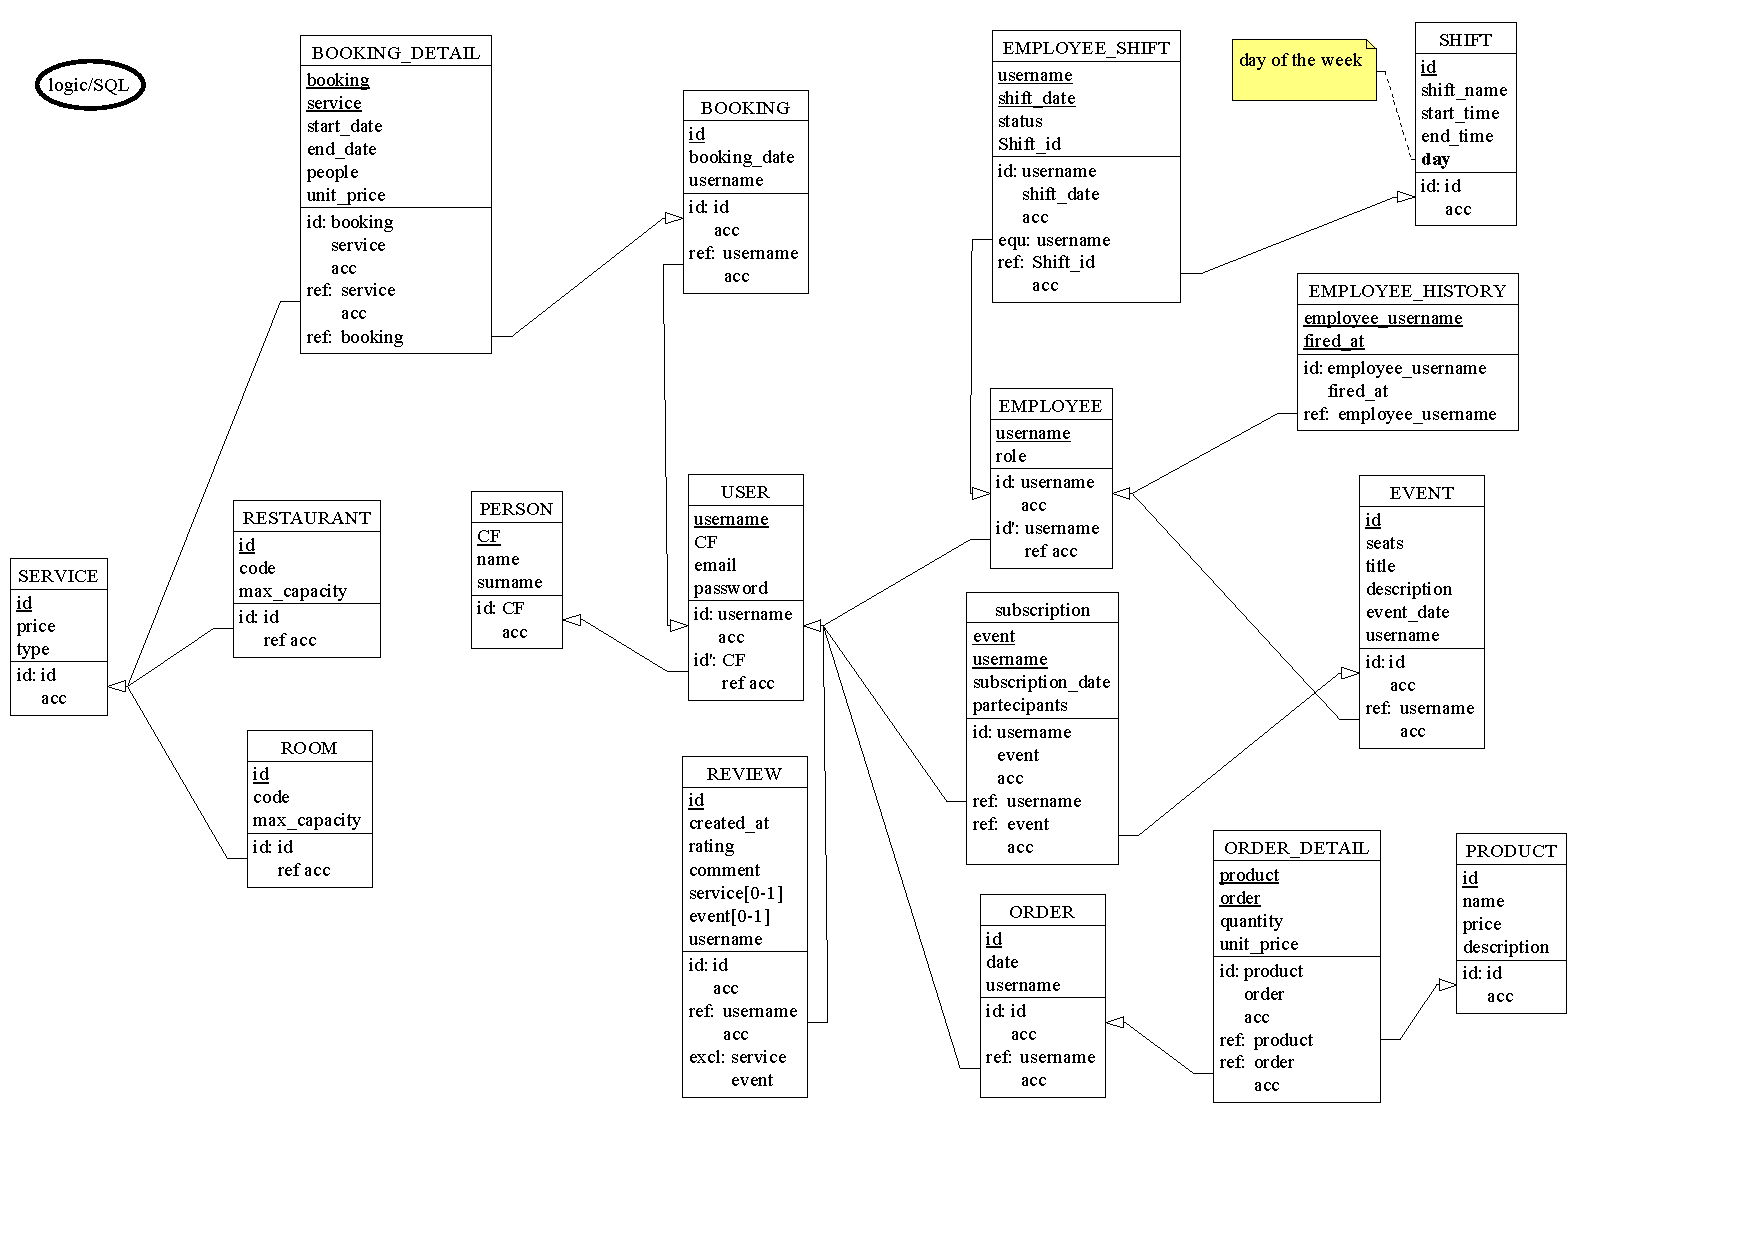
\includegraphics[width=\textwidth, trim=0 0 50pt 0]{./schemas/logic.pdf}
  \caption{Schema relazionale finale}
  \label{fig:schema-relazione}
\end{figure}
\newpage

\chapter{Progettazione della Base di Dati}
Una volta creato il nostro database, riportiamo di seguito una parte
del codice relazionale utilizzato per la sua implementazione.

\section{Check}
Sono stati utilizzati vincoli di tipo \texttt{CHECK} per definire
alcuni domini e assicurare
semplici proprietà degli attributi. Di seguito un esempio di vincolo
\texttt{CHECK} utilizzato
per assicurare che il prezzo di ogni prodotto sia maggiore zero:

% tex-fmt: off
\begin{sqlcode}[caption={},label={lst:check}]
CREATE TABLE PRODUCT (
    id INT AUTO_INCREMENT PRIMARY KEY,
    name VARCHAR(100) NOT NULL,
    description TEXT NOT NULL,
    price DECIMAL(8,2) NOT NULL CHECK (price > 0)
);
\end{sqlcode}
% tex-fmt: on

\section{Viste}
La seguente vista \texttt{Active\_Employees} restituisce l'elenco dei
dipendenti attivi, mostrando per ciascuno username, email, nome,
cognome e ruolo. Un dipendente è considerato attivo se il suo
username non compare nella tabella \texttt{Employee\_History}, che
traccia lo storico delle variazioni di stato.

% tex-fmt: off
\begin{sqlcode}[caption={},label={lst:view}]
CREATE VIEW active_employees AS
SELECT
    e.username,
    u.email,
    p.name,
    p.surname,
    e.role
FROM EMPLOYEE e
JOIN USER u ON e.username = u.username
JOIN PERSON p ON u.cf = p.cf
WHERE e.username NOT IN (
    SELECT username FROM EMPLOYEE_HISTORY
  );
\end{sqlcode}
% tex-fmt: on

\section{Trigger}
Esempio di trigger per vincolare le recensioni: impedisce di
recensire sia evento che servizio insieme, e consente la recensione
solo se l'utente ha partecipato all'evento (già svolto) o ha
usufruito del servizio.

% tex-fmt: off
\begin{sqlcode}[caption={},label={lst:trigger}]
DROP TRIGGER IF EXISTS trg_review_before_insert;
DELIMITER $$
CREATE TRIGGER trg_review_before_insert
BEFORE INSERT ON REVIEW
FOR EACH ROW
BEGIN
    DECLARE cnt INT DEFAULT 0;

    IF (NEW.event IS NOT NULL AND NEW.service IS NOT NULL) OR (NEW.event IS NULL AND NEW.service IS NULL) THEN
        SIGNAL SQLSTATE '45000'
            SET MESSAGE_TEXT = 'Set either event or service (not both) for the review.';
    END IF;

    IF NEW.event IS NOT NULL THEN
        SELECT COUNT(*)
            INTO cnt
            FROM EVENT e
            JOIN EVENT_SUBSCRIPTION es
                ON es.event = e.id
             AND es.`user` = NEW.`user`
         WHERE e.id = NEW.event
             AND e.event_date < CURDATE();

        IF cnt = 0 THEN
            SIGNAL SQLSTATE '45000'
                SET MESSAGE_TEXT = 'You can review the event only if you were subscribed and the event date is in the past.';
        END IF;
    END IF;

    IF NEW.service IS NOT NULL THEN
        SELECT COUNT(*)
            INTO cnt
      FROM BOOKING r
      JOIN BOOKING_DETAIL rd
        ON rd.booking = r.id
             AND rd.service = NEW.service
         WHERE r.username = NEW.`user`
             AND rd.end_date < NOW();

        IF cnt = 0 THEN
            SIGNAL SQLSTATE '45000'
                SET MESSAGE_TEXT = 'You can review the service only after you have used it (completed booking).';
        END IF;
    END IF;
END$$
DELIMITER ;
\end{sqlcode}
% tex-fmt: on

\section{Traduzione delle operazioni}
Vengono presentate le query SQL che implementano le principali
operazioni del sistema agriturismo. Le query sono state progettate
per essere efficienti e sfruttare gli indici e i vincoli definiti
nello schema. Di seguito sono riportate le principali operazioni
raggruppate per area funzionale: statistiche, prenotazioni,
recensioni, iscrizioni eventi, autenticazione e gestione ordini.

\subsection{Visualizzazione statistiche dashboard}
Le seguenti query sono utilizzate per popolare la dashboard
amministrativa con le metriche principali del sistema.

\subsubsection{Migliori servizi per prenotazioni}
Analizza le prenotazioni per identificare i servizi più richiesti,
distinguendo tra ristoranti e camere attraverso un'articolata
procedura di join e raggruppamento.

% tex-fmt: off
\begin{sqlcode}[caption={}]
SELECT CASE
    WHEN s.type = 'RESTAURANT' THEN CONCAT('Restaurant - ', r.code)
    WHEN s.type = 'ROOM' THEN CONCAT('Room - ', ro.code)
    ELSE s.type
  END AS service_name,
  COUNT(rd.service) AS booking_count
FROM SERVICE AS s
LEFT JOIN RESTAURANT AS r ON s.id = r.service
LEFT JOIN ROOM AS ro ON s.id = ro.service
JOIN BOOKING_DETAIL AS rd ON s.id = rd.service
GROUP BY s.id, s.type, r.code, ro.code
ORDER BY booking_count DESC
LIMIT 5;
\end{sqlcode}
% tex-fmt: on

\subsubsection{Migliori prodotti per quantità venduta}
Prodotti più venduti in base alla quantità totale ordinata.

% tex-fmt: off
\begin{sqlcode}[caption={}]
SELECT
  p.name AS product_name,
  SUM(od.quantity) AS total_quantity
FROM PRODUCT AS p
JOIN ORDER_DETAIL AS od ON p.id = od.product
GROUP BY p.id, p.name
ORDER BY total_quantity DESC
LIMIT 5;
\end{sqlcode}
% tex-fmt: on

\newpage
\subsubsection{Migliori eventi per partecipanti}
Determina gli eventi con il maggior numero di partecipanti totali.

% tex-fmt: off
\begin{sqlcode}[caption={}]
SELECT
  e.title AS event_title,
  e.event_date,
  SUM(es.participants) AS total_participants
FROM EVENT AS e
JOIN EVENT_SUBSCRIPTION AS es ON e.id = es.event
GROUP BY e.id, e.title, e.event_date
ORDER BY total_participants DESC
LIMIT 5;
\end{sqlcode}
% tex-fmt: on

\subsubsection{Migliori prodotti per fatturato}
Calcola i 5 prodotti che generano il maggior fatturato.

% tex-fmt: off
\begin{sqlcode}[caption={}]
SELECT
  p.name AS product_name,
  SUM(od.quantity * od.unit_price) AS total_revenue
FROM PRODUCT AS p
JOIN ORDER_DETAIL AS od ON p.id = od.product
GROUP BY p.id, p.name
ORDER BY total_revenue DESC
LIMIT 5;
\end{sqlcode}
% tex-fmt: on

\subsubsection{Fatturato totale}
Calcolo del ricavo complessivo generato dalle vendite dei prodotti.

% tex-fmt: off
\begin{sqlcode}[caption={}]
SELECT
    (SELECT SUM(quantity * unit_price) FROM ORDER_DETAIL)
  + (SELECT SUM(unit_price * DATEDIFF(end_date, start_date)) FROM BOOKING_DETAIL)
  AS fatturato_totale;
\end{sqlcode}
% tex-fmt: on

\subsubsection{Statistiche generali del sistema}
Query composita che fornisce un riepilogo completo delle metriche di
sistema tramite sottoselezioni multiple, aggregando dati da diverse
tabelle per offrire una visione d'insieme immediata.

% tex-fmt: off
\begin{sqlcode}[caption={}]
SELECT
  (SELECT COUNT(*) FROM USER) AS total_customers,
  (SELECT COUNT(*) FROM EMPLOYEE) AS total_employees,
  (SELECT COUNT(*) FROM ORDERS) AS total_orders,
  (SELECT ROUND(SUM(od.quantity * od.unit_price), 2) FROM ORDER_DETAIL AS od) AS total_revenue,
  (SELECT COUNT(*) FROM BOOKING) AS total_bookings;
\end{sqlcode}
% tex-fmt: on

\newpage
\subsection{Prenotazione servizi}
Le principali query per la prenotazione di servizi, come camere e
tavoli al ristorante, includono la verifica della disponibilità, la
creazione della prenotazione e la gestione dei dettagli associati,
garantendo il rispetto dei vincoli di capacità e delle regole
temporali definite dal sistema.

\subsubsection{Verifica disponibilità camere}
La disponibilità delle camere viene verificata analizzando le
prenotazioni esistenti e selezionando solo quelle con capacità
sufficiente e libere nel periodo richiesto. Il controllo si basa
sulla non sovrapposizione temporale tra le prenotazioni già
registrate e l'intervallo desiderato, così da garantire che la camera
sia effettivamente disponibile.

% tex-fmt: off
\begin{sqlcode}[caption={}]
SELECT
  ro.code AS room,
  s.price AS price,
  ro.max_capacity
FROM ROOM AS ro
JOIN SERVICE AS s
  ON s.id = ro.service
WHERE
  ro.max_capacity >= @n_people
  AND ro.service NOT IN (
    SELECT rd.service
  FROM BOOKING_DETAIL AS rd
    WHERE NOT (rd.end_date <= @start_date OR rd.start_date >= @end_date)
  );
\end{sqlcode}
% tex-fmt: on

\subsubsection{Verifica disponibilità tavoli}
Calcola i posti disponibili considerando le prenotazioni esistenti
che si sovrappongono all'intervallo richiesto, utilizzando un left
join condizionato e una clausola HAVING per filtrare i ristoranti con
posti sufficienti.

% tex-fmt: off
\begin{sqlcode}[caption={}]
SELECT
  r.code AS restaurant,
  s.price AS price,
  r.max_capacity,
  (r.max_capacity - IFNULL(SUM(rd.people), 0)) AS available_seats
FROM RESTAURANT AS r
JOIN SERVICE AS s ON s.id = r.service
LEFT JOIN BOOKING_DETAIL AS rd ON rd.service = r.service
  AND NOT (rd.end_date <= @start_date OR rd.start_date >= @end_date)
GROUP BY r.service, r.code, s.price, r.max_capacity
HAVING available_seats >= @n_people;
\end{sqlcode}
% tex-fmt: on

\newpage
\subsection{Gestione recensioni}
Gli utenti possono recensire solo eventi conclusi a cui hanno
partecipato o servizi già prenotati e utilizzati, garantendo
valutazioni autentiche.

\subsubsection{Inserimento recensione evento}
Questa query consente di inserire una recensione per un evento solo
se l'utente è iscritto, l'evento si è concluso e non esiste già una
recensione per quell'evento da parte dello stesso utente. In questo
modo si garantisce la correttezza e l'integrità dei dati.

% tex-fmt: off
\begin{sqlcode}[caption={}]
INSERT INTO REVIEW (user, event, rating, comment)
SELECT
  'mrossi' AS user,
  e.id AS event,
  5 AS rating,
  'Amazing experience! Will definitely come again.' AS comment
FROM EVENT AS e
INNER JOIN EVENT_SUBSCRIPTION AS es ON e.id = es.event
  AND es.user = 'mrossi'
WHERE
  e.title = 'Farm Open Day'
  AND e.event_date < CURDATE()
    AND NOT EXISTS (
      SELECT 1
      FROM REVIEW AS r
      WHERE r.user = 'mrossi' AND r.event = e.id
  )
LIMIT 1;
\end{sqlcode}
% tex-fmt: on

\subsubsection{Inserimento recensione servizio}
Consente di inserire una recensione su un servizio solo se l'utente
ha completato una prenotazione per quel servizio e non esiste già una
recensione associata, garantendo così la correttezza referenziale ed
evitando duplicati.

% tex-fmt: off
\begin{sqlcode}[caption={}]
INSERT INTO REVIEW (user, service, rating, comment)
SELECT
  'aneri' AS user,
  s.id AS service,
  4 AS rating,
  'Good service and friendly staff.' AS comment
FROM SERVICE AS s
INNER JOIN BOOKING_DETAIL AS bd ON s.id = rd.service
INNER JOIN BOOKING AS b ON bd.booking = b.id
WHERE
  r.username = 'aneri'
  AND bd.end_date < NOW()
  AND s.type = 'RESTAURANT'
  AND NOT EXISTS (
    SELECT 1

    FROM REVIEW AS rev
    WHERE rev.user = 'aneri' AND rev.service = s.id
  )
LIMIT 1;
\end{sqlcode}
% tex-fmt: on

\subsubsection{Aggiornamento recensione}
Modifica il voto e il commento di una recensione esistente.

% tex-fmt: off
\begin{sqlcode}[caption={}]
UPDATE REVIEW
SET
  rating = 4,
  comment = 'Very good event, but could use more activities. Overall enjoyed it!',
  created_at = NOW()
WHERE
  user = 'mrossi'
    AND event = (
    SELECT id
    FROM EVENT
    WHERE title = 'Farm Open Day'
    )
  AND id IS NOT NULL;
\end{sqlcode}
% tex-fmt: on

\subsection{Gestione iscrizioni eventi}
Le operazioni sulle iscrizioni agli eventi includono la registrazione
di nuovi partecipanti, l'aggiornamento del numero di iscritti e la
cancellazione delle iscrizioni. Il sistema garantisce che il numero
totale di partecipanti non superi la capienza dell'evento e consente
agli utenti di modificare o annullare la propria iscrizione fino
all'inizio dell'evento.

\subsubsection{Update e Iscrizione utente a evento}
Permette a un utente di iscriversi a un evento specificando il numero
di partecipanti. Il meccanismo "ON DUPLICATE KEY UPDATE" trasforma
l'insert in un update che modifica solo il numero di partecipanti,
nel caso in cui l'utente abbia già effettuato un'iscrizione al dato evento.

% tex-fmt: off
\begin{sqlcode}[caption={}]
INSERT INTO EVENT_SUBSCRIPTION (event, user, participants)
SELECT
  e.id,
  u.username,
  4
FROM EVENT AS e
CROSS JOIN USER AS u
WHERE e.title = 'Harvest Festival' AND u.username = 'lblu'
ON DUPLICATE KEY UPDATE participants = 4;
\end{sqlcode}
% tex-fmt: on

\newpage
\subsection{Esecuzione prenotazioni confermate}
Le prenotazioni di servizi (camere e ristoranti) vengono gestite
tramite query che verificano la disponibilità, creano la prenotazione
principale e aggiungono i dettagli relativi al servizio scelto. Il
sistema assicura che non vi siano sovrapposizioni e che la capacità
sia rispettata, garantendo integrità e correttezza dei dati.

\subsubsection{Creazione prenotazione principale}
Crea il record principale di prenotazione per un utente, con un
controllo che evita la creazione di prenotazioni duplicate nella
stessa giornata.

% tex-fmt: off
\begin{sqlcode}[caption={}]
INSERT INTO BOOKING (username, booking_date)
SELECT
  'gverdi',
  NOW()
WHERE NOT EXISTS (
  SELECT 1
  FROM BOOKING
  WHERE
    username = 'gverdi'
  AND DATE(booking_date) = CURDATE()
  );
\end{sqlcode}
% tex-fmt: on

\subsubsection{Prenotazione tavolo ristorante}
Prenotazione di tavoli al ristorante, con join sulla tabella
RESTAURANT per identificare correttamente il servizio.
% tex-fmt: off
\begin{sqlcode}[caption={}]
SET @new_booking_id = LAST_INSERT_ID();

INSERT INTO BOOKING_DETAIL (booking, service, start_date, end_date, people, unit_price)
SELECT
  @new_booking_id AS booking,
  s.id AS service,
  '2024-01-25 19:00:00' AS start_date,
  '2024-01-25 21:00:00' AS end_date,
  2 AS people,
  s.price AS unit_price
FROM SERVICE AS s
INNER JOIN RESTAURANT AS r ON s.id = r.service
WHERE r.code = 'T01'
LIMIT 1;
\end{sqlcode}
% tex-fmt: on

\newpage
\subsubsection{Prenotazione camera con controllo duplicati}
Gestione della prenotazione di una camera, con creazione della
prenotazione principale e dei dettagli. Sono previsti controlli per
evitare duplicati e viene gestito correttamente l'ID generato per la
prenotazione.

% tex-fmt: off
\begin{sqlcode}[caption={}]
INSERT INTO BOOKING (username, booking_date)
SELECT 'fbianchi', DATE_ADD(NOW(), INTERVAL 1 HOUR)
WHERE NOT EXISTS (
  SELECT 1 FROM BOOKING
  WHERE username = 'fbianchi'
  AND DATE(booking_date) = CURDATE()
);

SET @room_booking_id = LAST_INSERT_ID();

INSERT INTO BOOKING_DETAIL (booking, service, start_date, end_date, people, unit_price)
SELECT
  @room_booking_id as booking,
  s.id as service,
  '2024-01-26 15:00:00' as start_date,
  '2024-01-28 11:00:00' as end_date,
  2 as people,
  s.price as unit_price
FROM SERVICE s
INNER JOIN ROOM r ON s.id = r.service
WHERE r.code = 'R03'
LIMIT 1;
\end{sqlcode}
% tex-fmt: on

\newpage
\subsection{Eliminazione prenotazioni e iscrizioni}
Le operazioni di eliminazione permettono agli utenti e agli
amministratori di rimuovere prenotazioni di servizi e iscrizioni agli
eventi, garantendo il rispetto dei vincoli temporali e di integrità
referenziale. È possibile cancellare una prenotazione solo se non è
già iniziata, mentre le iscrizioni agli eventi possono essere
annullate fino all'inizio dell'evento. Queste funzionalità assicurano
una gestione sicura e corretta delle risorse e delle partecipazioni.

\subsubsection{Eliminazione prenotazione servizio}
Permette di cancellare una prenotazione di servizio esistente,
rimuovendo prima i dettagli della prenotazione per rispettare i
vincoli di integrità referenziale e successivamente il record
principale della prenotazione.

% tex-fmt: off
\begin{sqlcode}[caption={}]
DELETE FROM BOOKING_DETAIL
WHERE booking = @booking_id;

DELETE FROM BOOKING
WHERE id = @booking_id
AND username = @username;
\end{sqlcode}
% tex-fmt: on

\subsubsection{Eliminazione iscrizione evento}
Rimuove l'iscrizione di un utente a un evento specifico, verificando
che l'iscrizione esista e che l'evento non sia già iniziato; in
questo modo è consentita la cancellazione solo per eventi futuri.

% tex-fmt: off
\begin{sqlcode}[caption={}]
DELETE FROM EVENT_SUBSCRIPTION
WHERE
  user = @username
  AND event = @event_id
  AND EXISTS (
    SELECT 1
    FROM EVENT AS e
    WHERE
      e.id = @event_id
      AND e.event_date > CURDATE()
  );
\end{sqlcode}
% tex-fmt: on

\subsubsection{Eliminazione prenotazione con controllo temporale}
L'eliminazione di una prenotazione è consentita solo se non è già
iniziata; viene implementato un controllo temporale che previene la
cancellazione di prenotazioni in corso o concluse.

% tex-fmt: off
\begin{sqlcode}[caption={}]
DELETE FROM BOOKING
WHERE
  id = @booking_id
  AND username = @username
  AND NOT EXISTS (
    SELECT 1
  FROM BOOKING_DETAIL AS bd
    WHERE
      bd.booking = @booking_id
      AND bd.start_date <= NOW()
  );
\end{sqlcode}
% tex-fmt: on

\newpage
\subsection{Autenticazione utente}
L'autenticazione utente consente l'accesso sicuro alla piattaforma
tramite verifica di username e password. Per distinguere tra clienti
e dipendenti, viene utilizzata la vista \texttt{active\_employees}:
se il campo \texttt{role} restituito dalla vista è \texttt{NULL},
l'utente è considerato un cliente normale; se invece è valorizzato,
l'utente è un dipendente attivo e il ruolo viene mostrato.

\subsubsection{Verifica credenziali di login}
La query seguente verifica le credenziali di login e determina il
profilo utente, sfruttando la vista \texttt{active\_employees} per
identificare i dipendenti attivi.

% tex-fmt: off
\begin{sqlcode}[caption={}]
SELECT
  u.username,
  u.email,
  p.name,
  p.surname,
  CASE WHEN ae.role IS NOT NULL THEN 'employee' ELSE 'customer' END AS user_type,
  ae.role AS employee_role
FROM USER AS u
JOIN PERSON AS p ON u.cf = p.cf
LEFT JOIN active_employees AS ae ON u.username = ae.username
WHERE u.username = 'mrossi' OR u.email = 'mrossi@farm.com';
\end{sqlcode}
% tex-fmt: on

\newpage
\subsection{Gestione ordini prodotti}
Gli ordini prodotti vengono gestiti tramite una transazione che crea
l'ordine principale e inserisce i dettagli dei prodotti selezionati,
con quantità e prezzo corrente. Il sistema assicura che ogni ordine
sia associato all'utente e che i dati siano registrati in modo consistente.

\subsubsection{Creazione nuovo ordine}
La seguente procedura crea un nuovo ordine, recupera automaticamente
l'ID generato e inserisce i prodotti con i prezzi correnti, gestendo
tutta la logica di ordine in un'unica sequenza di operazioni.

% tex-fmt: off
\begin{sqlcode}[caption={}]
SET @new_order_id = LAST_INSERT_ID();

INSERT INTO ORDER_DETAIL (order, product, quantity, unit_price)
SELECT
  @new_order_id AS order_id,
  p.id AS product_id,
  3 AS quantity,
  p.price AS unit_price
FROM PRODUCT AS p
WHERE p.name = 'Farm Eggs (12 pcs)'
LIMIT 1;

INSERT INTO ORDER_DETAIL (order, product, quantity, unit_price)
SELECT
  @new_order_id AS order_id,
  p.id AS product_id,
  2 AS quantity,
  p.price AS unit_price
FROM PRODUCT AS p
WHERE p.name = 'Fresh Bread'
LIMIT 1;

INSERT INTO ORDER_DETAIL (order, product, quantity, unit_price)
SELECT
  @new_order_id AS order_id,
  p.id AS product_id,
  1 AS quantity,
  p.price AS unit_price
FROM PRODUCT AS p
WHERE p.name = 'Honey Jar (500g)'
LIMIT 1;
\end{sqlcode}
% tex-fmt: on

\chapter{Progettazione dell'applicazione}
L'applicazione è stata sviluppata con il framework \textbf{Django},
che gestisce routing,
database e autenticazione in modo sicuro e scalabile.

\section{Barra di Navigazione}
La \textbf{barra di navigazione} permette un accesso rapido alle
principali sezioni del sito,
come prodotti, eventi, servizi, area personale e funzioni amministrative.

\begin{figure}[H]
  \centering
  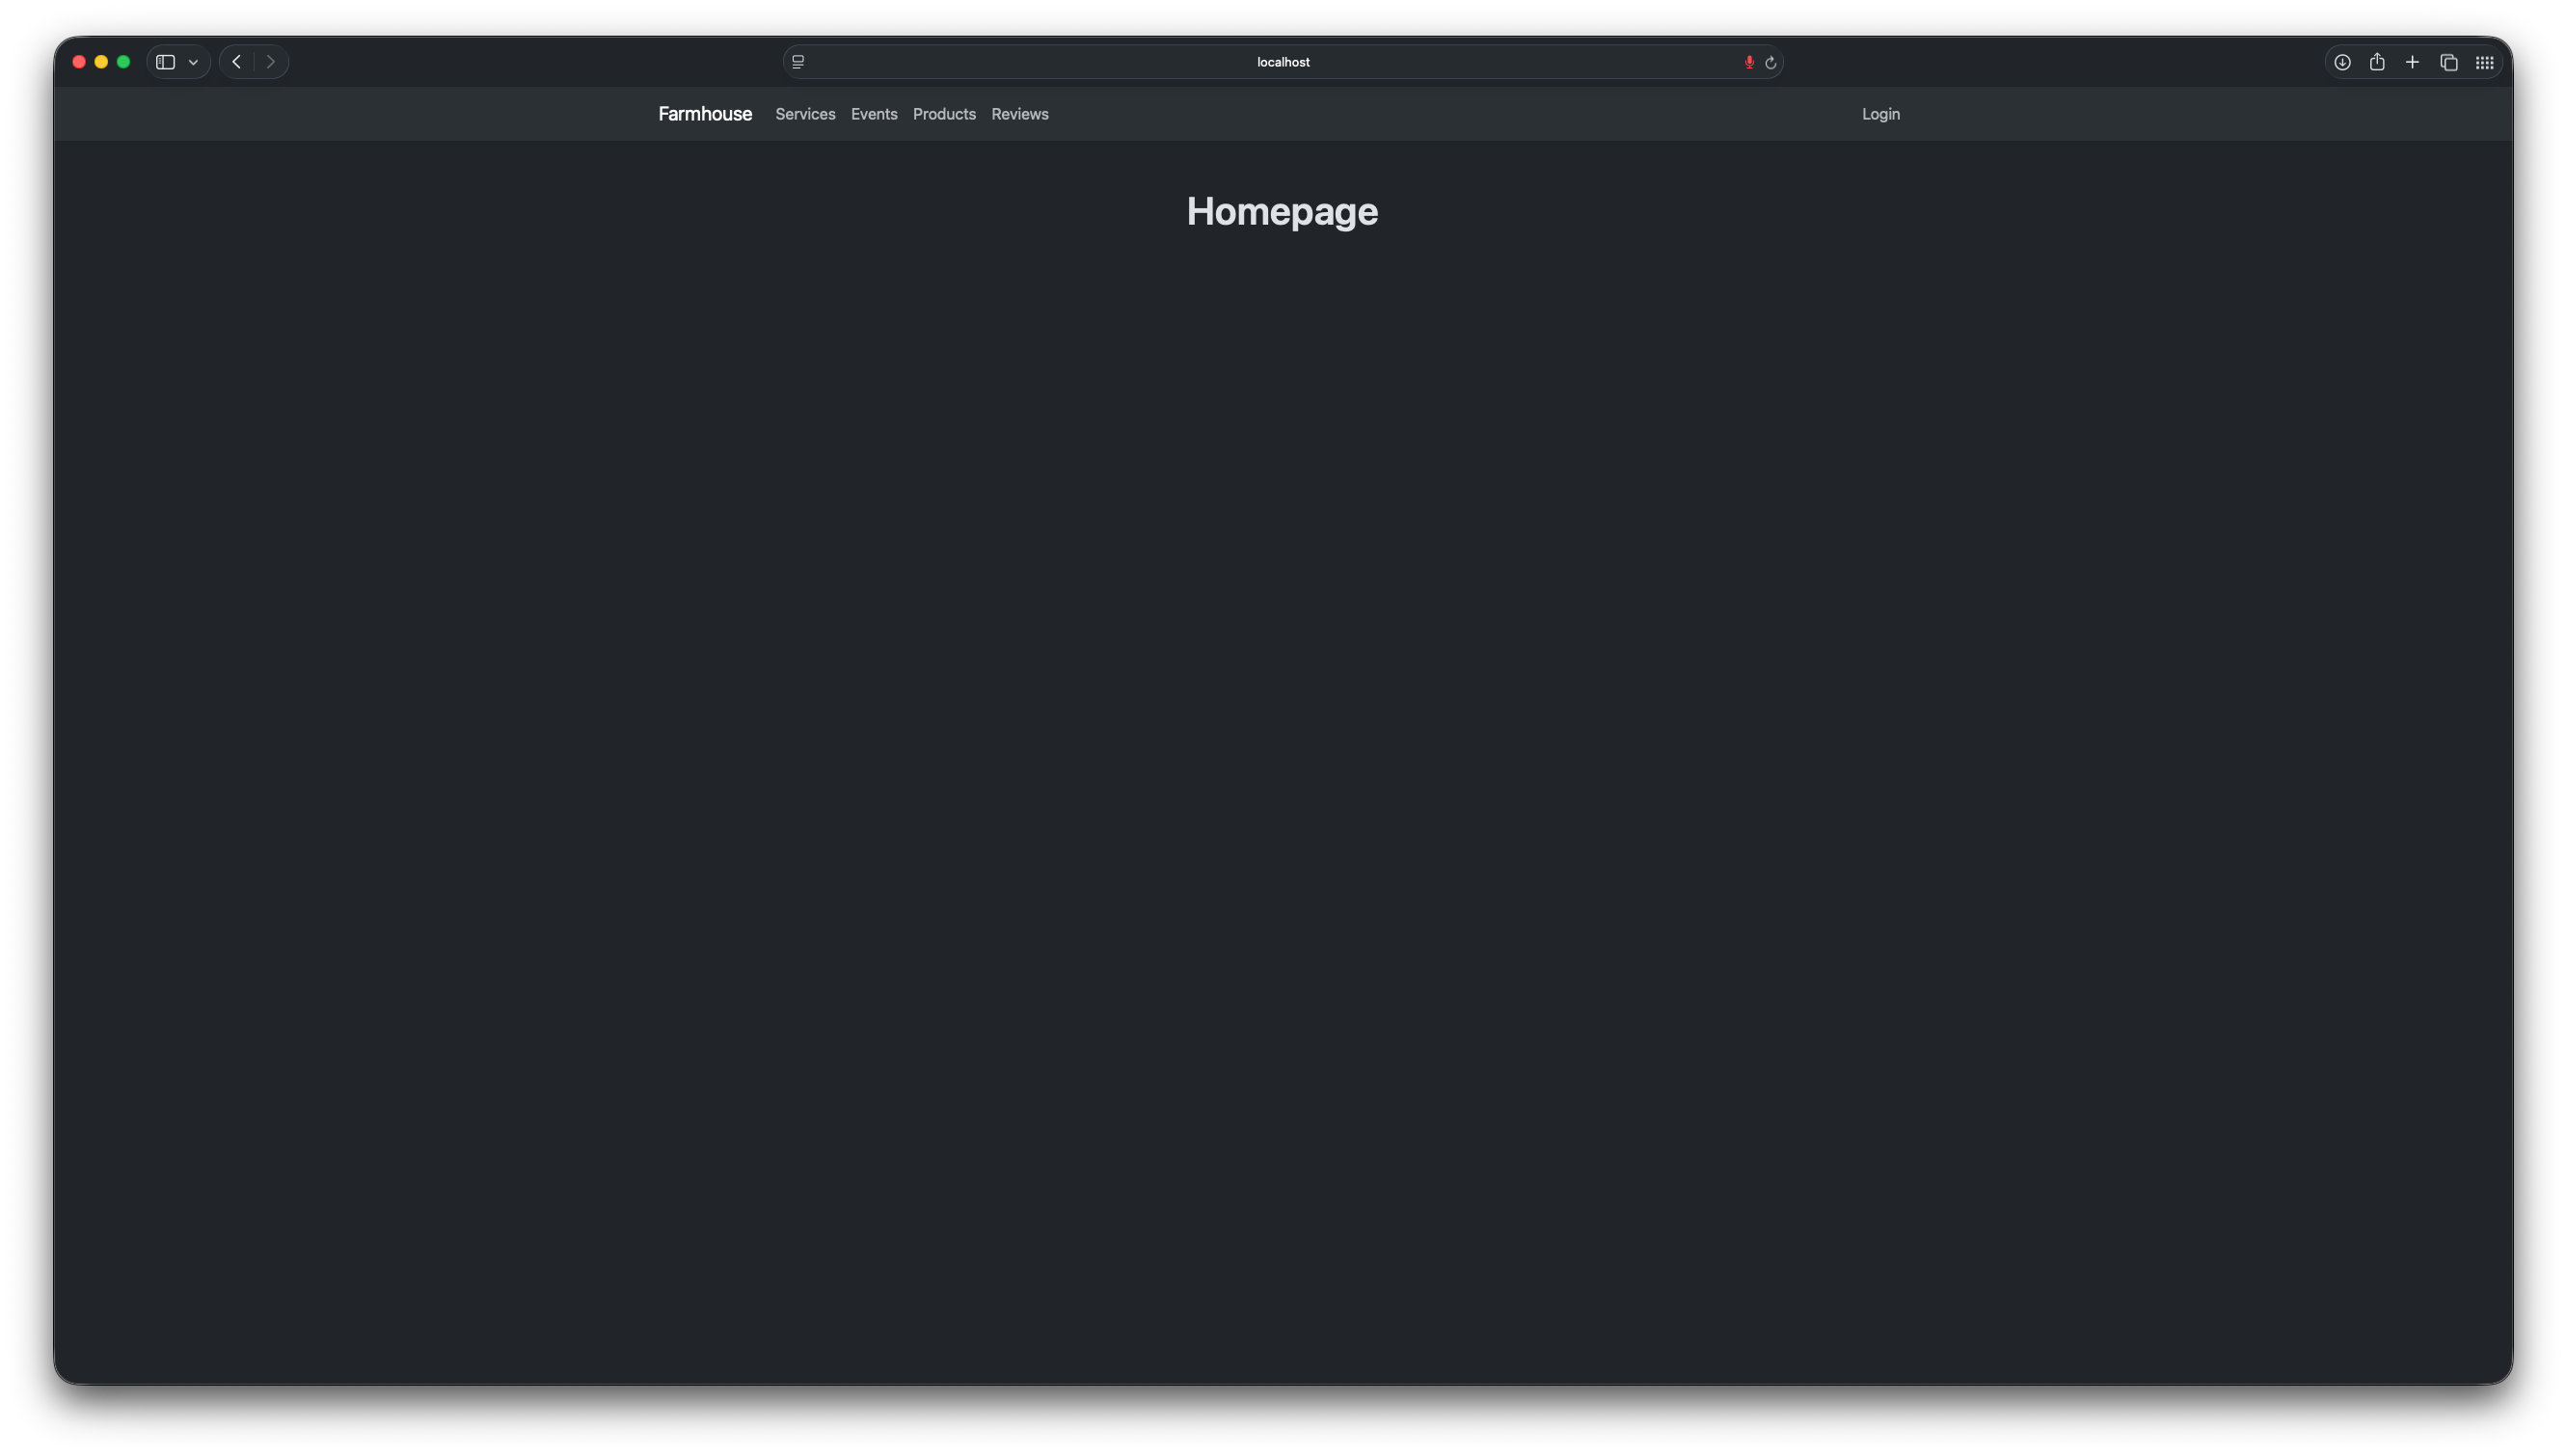
\includegraphics[width=\textwidth, trim=0 0 0 0]{./img/navbar.png}
  \caption{Barra di navigazione}
  \label{fig:navbar}
\end{figure}

\newpage
\subsection*{Login}

Il form di login consente agli utenti registrati di accedere
rapidamente alla piattaforma inserendo username e
password. Il sistema verifica le credenziali e, in caso di errore,
mostra un messaggio di avviso.

\begin{figure}[H]
  \centering
  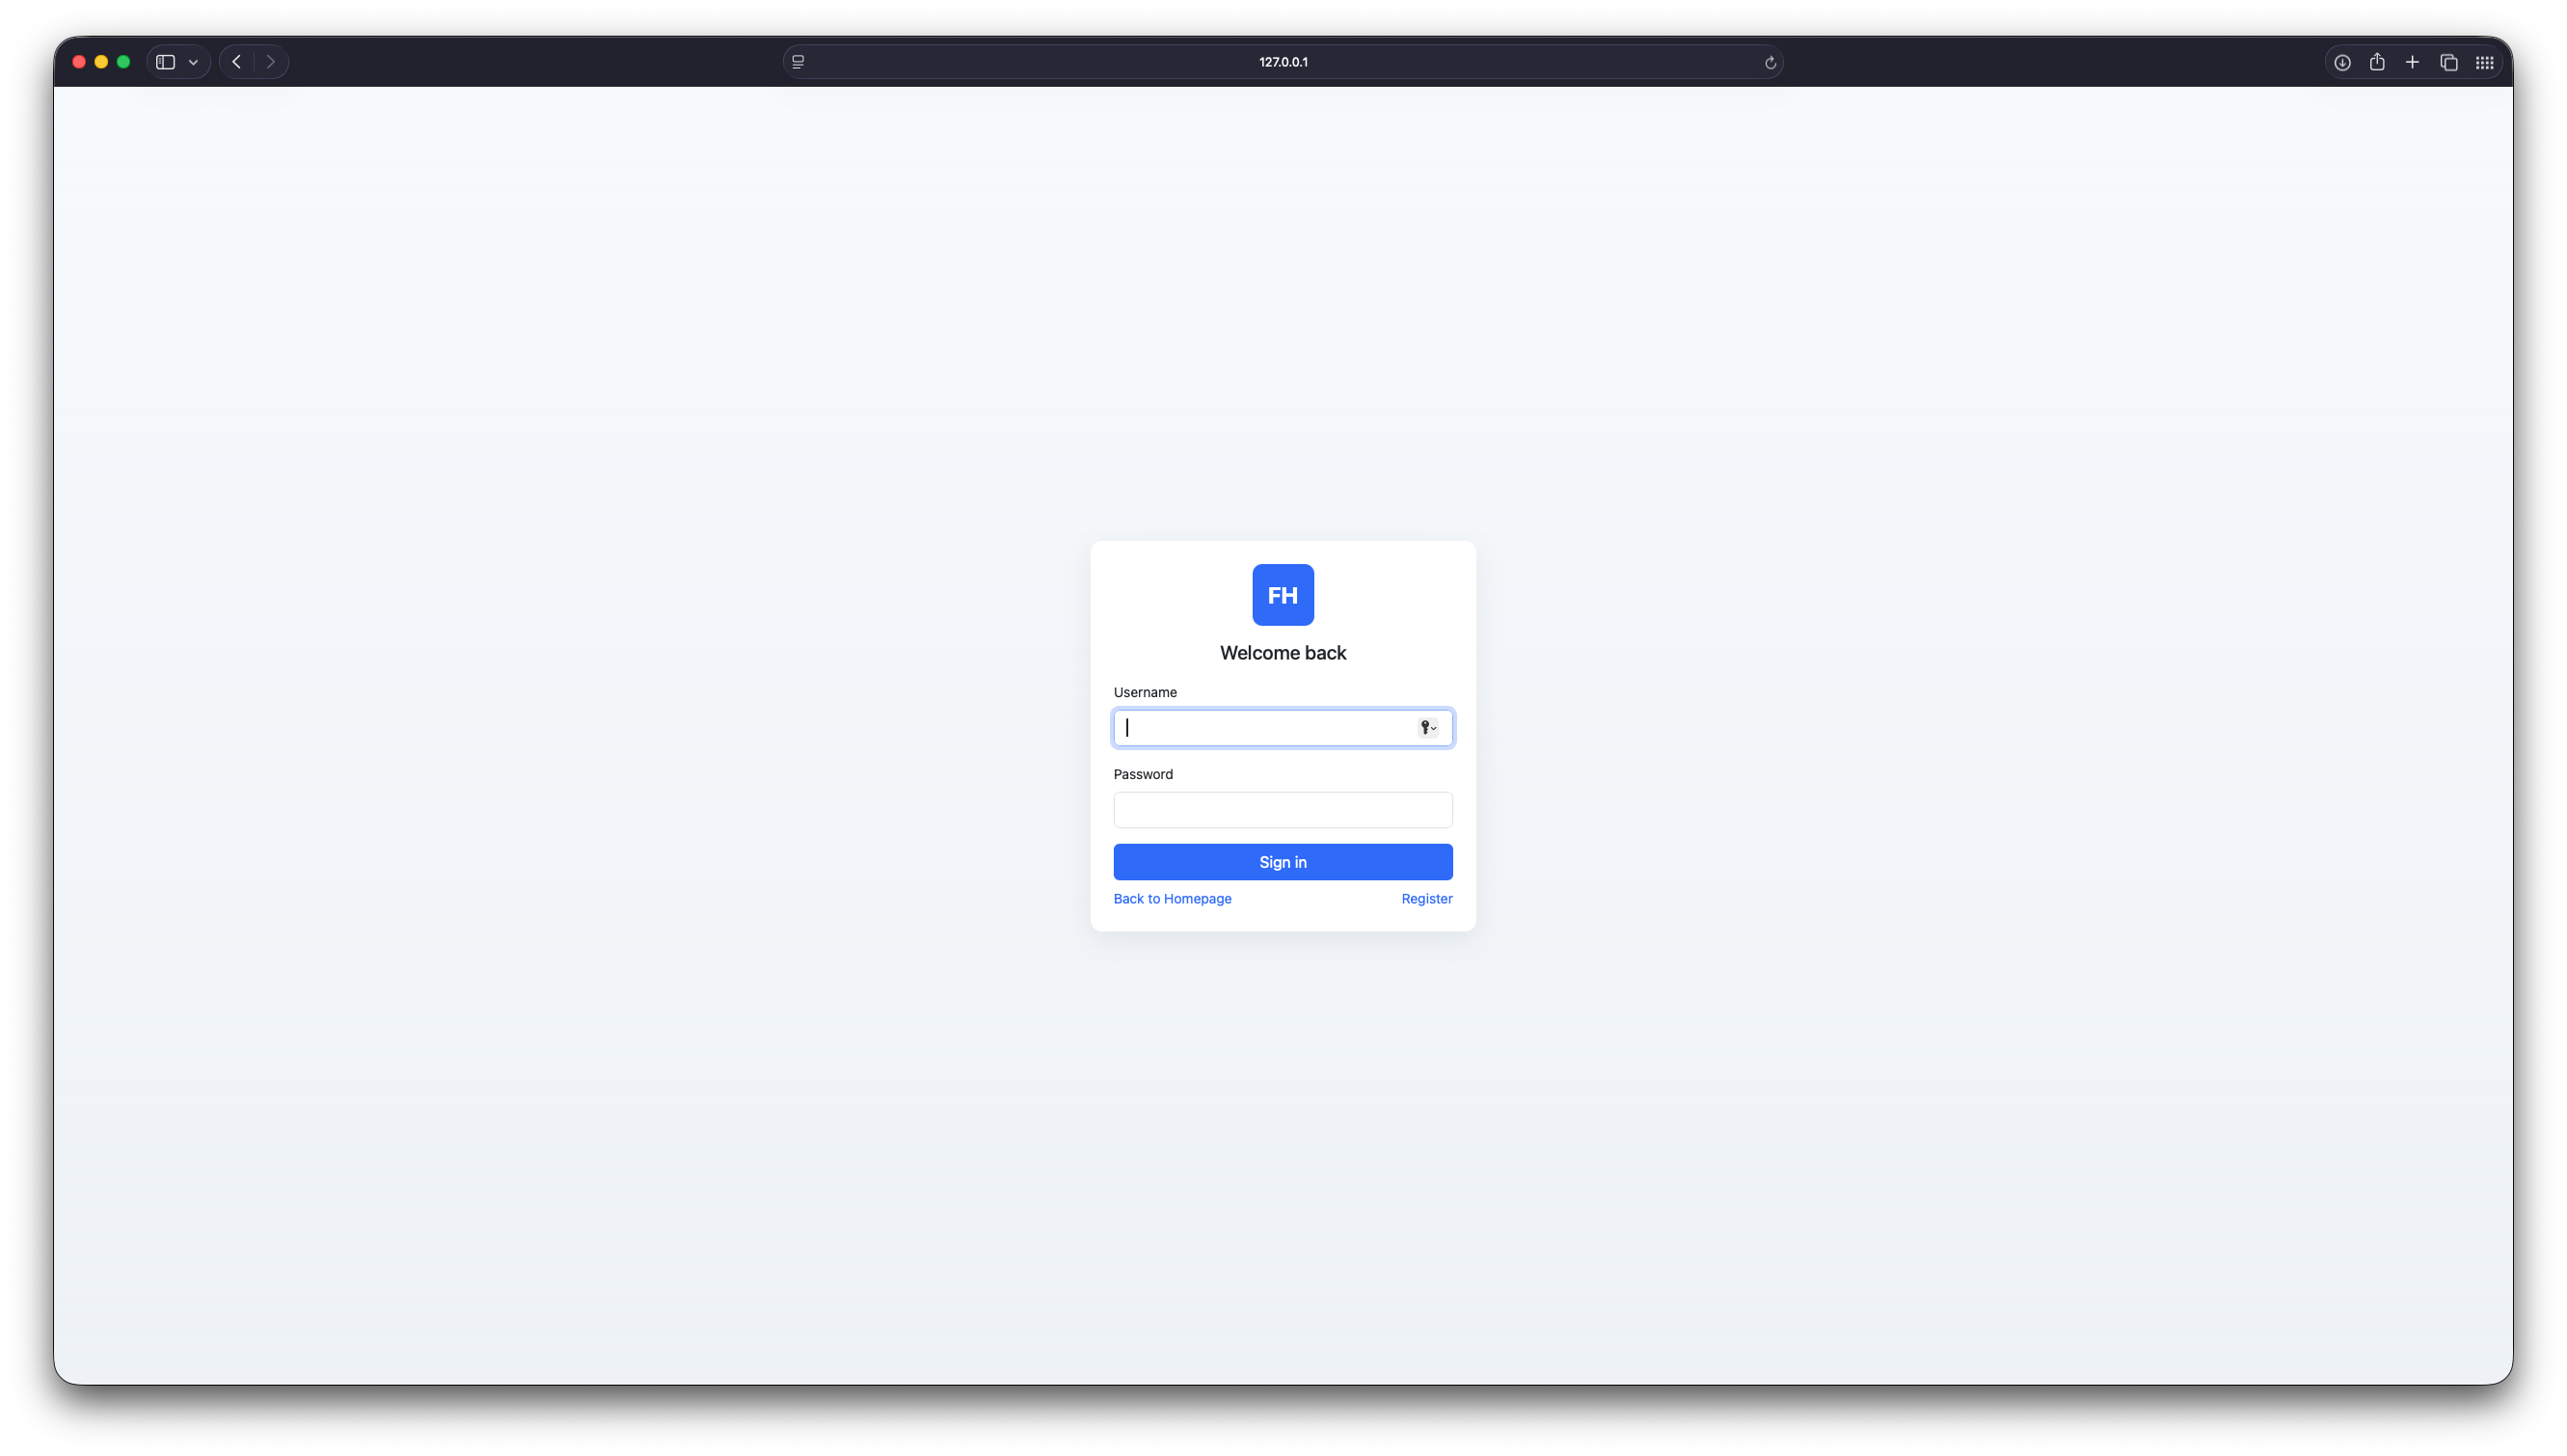
\includegraphics[width=\textwidth, trim=0 0 0 0]{./img/login.png}
  \vspace{-1em}
  \label{fig:login}
\end{figure}

\subsection*{Registrazione}
Anche per registrarsi è disponibile un form semplice e intuitivo, che
permette agli utenti di creare un nuovo
account inserendo i dati richiesti. Dopo la registrazione, l'utente
potrà accedere a tutte le funzionalità della
piattaforma.

\begin{figure}[H]
  \centering
  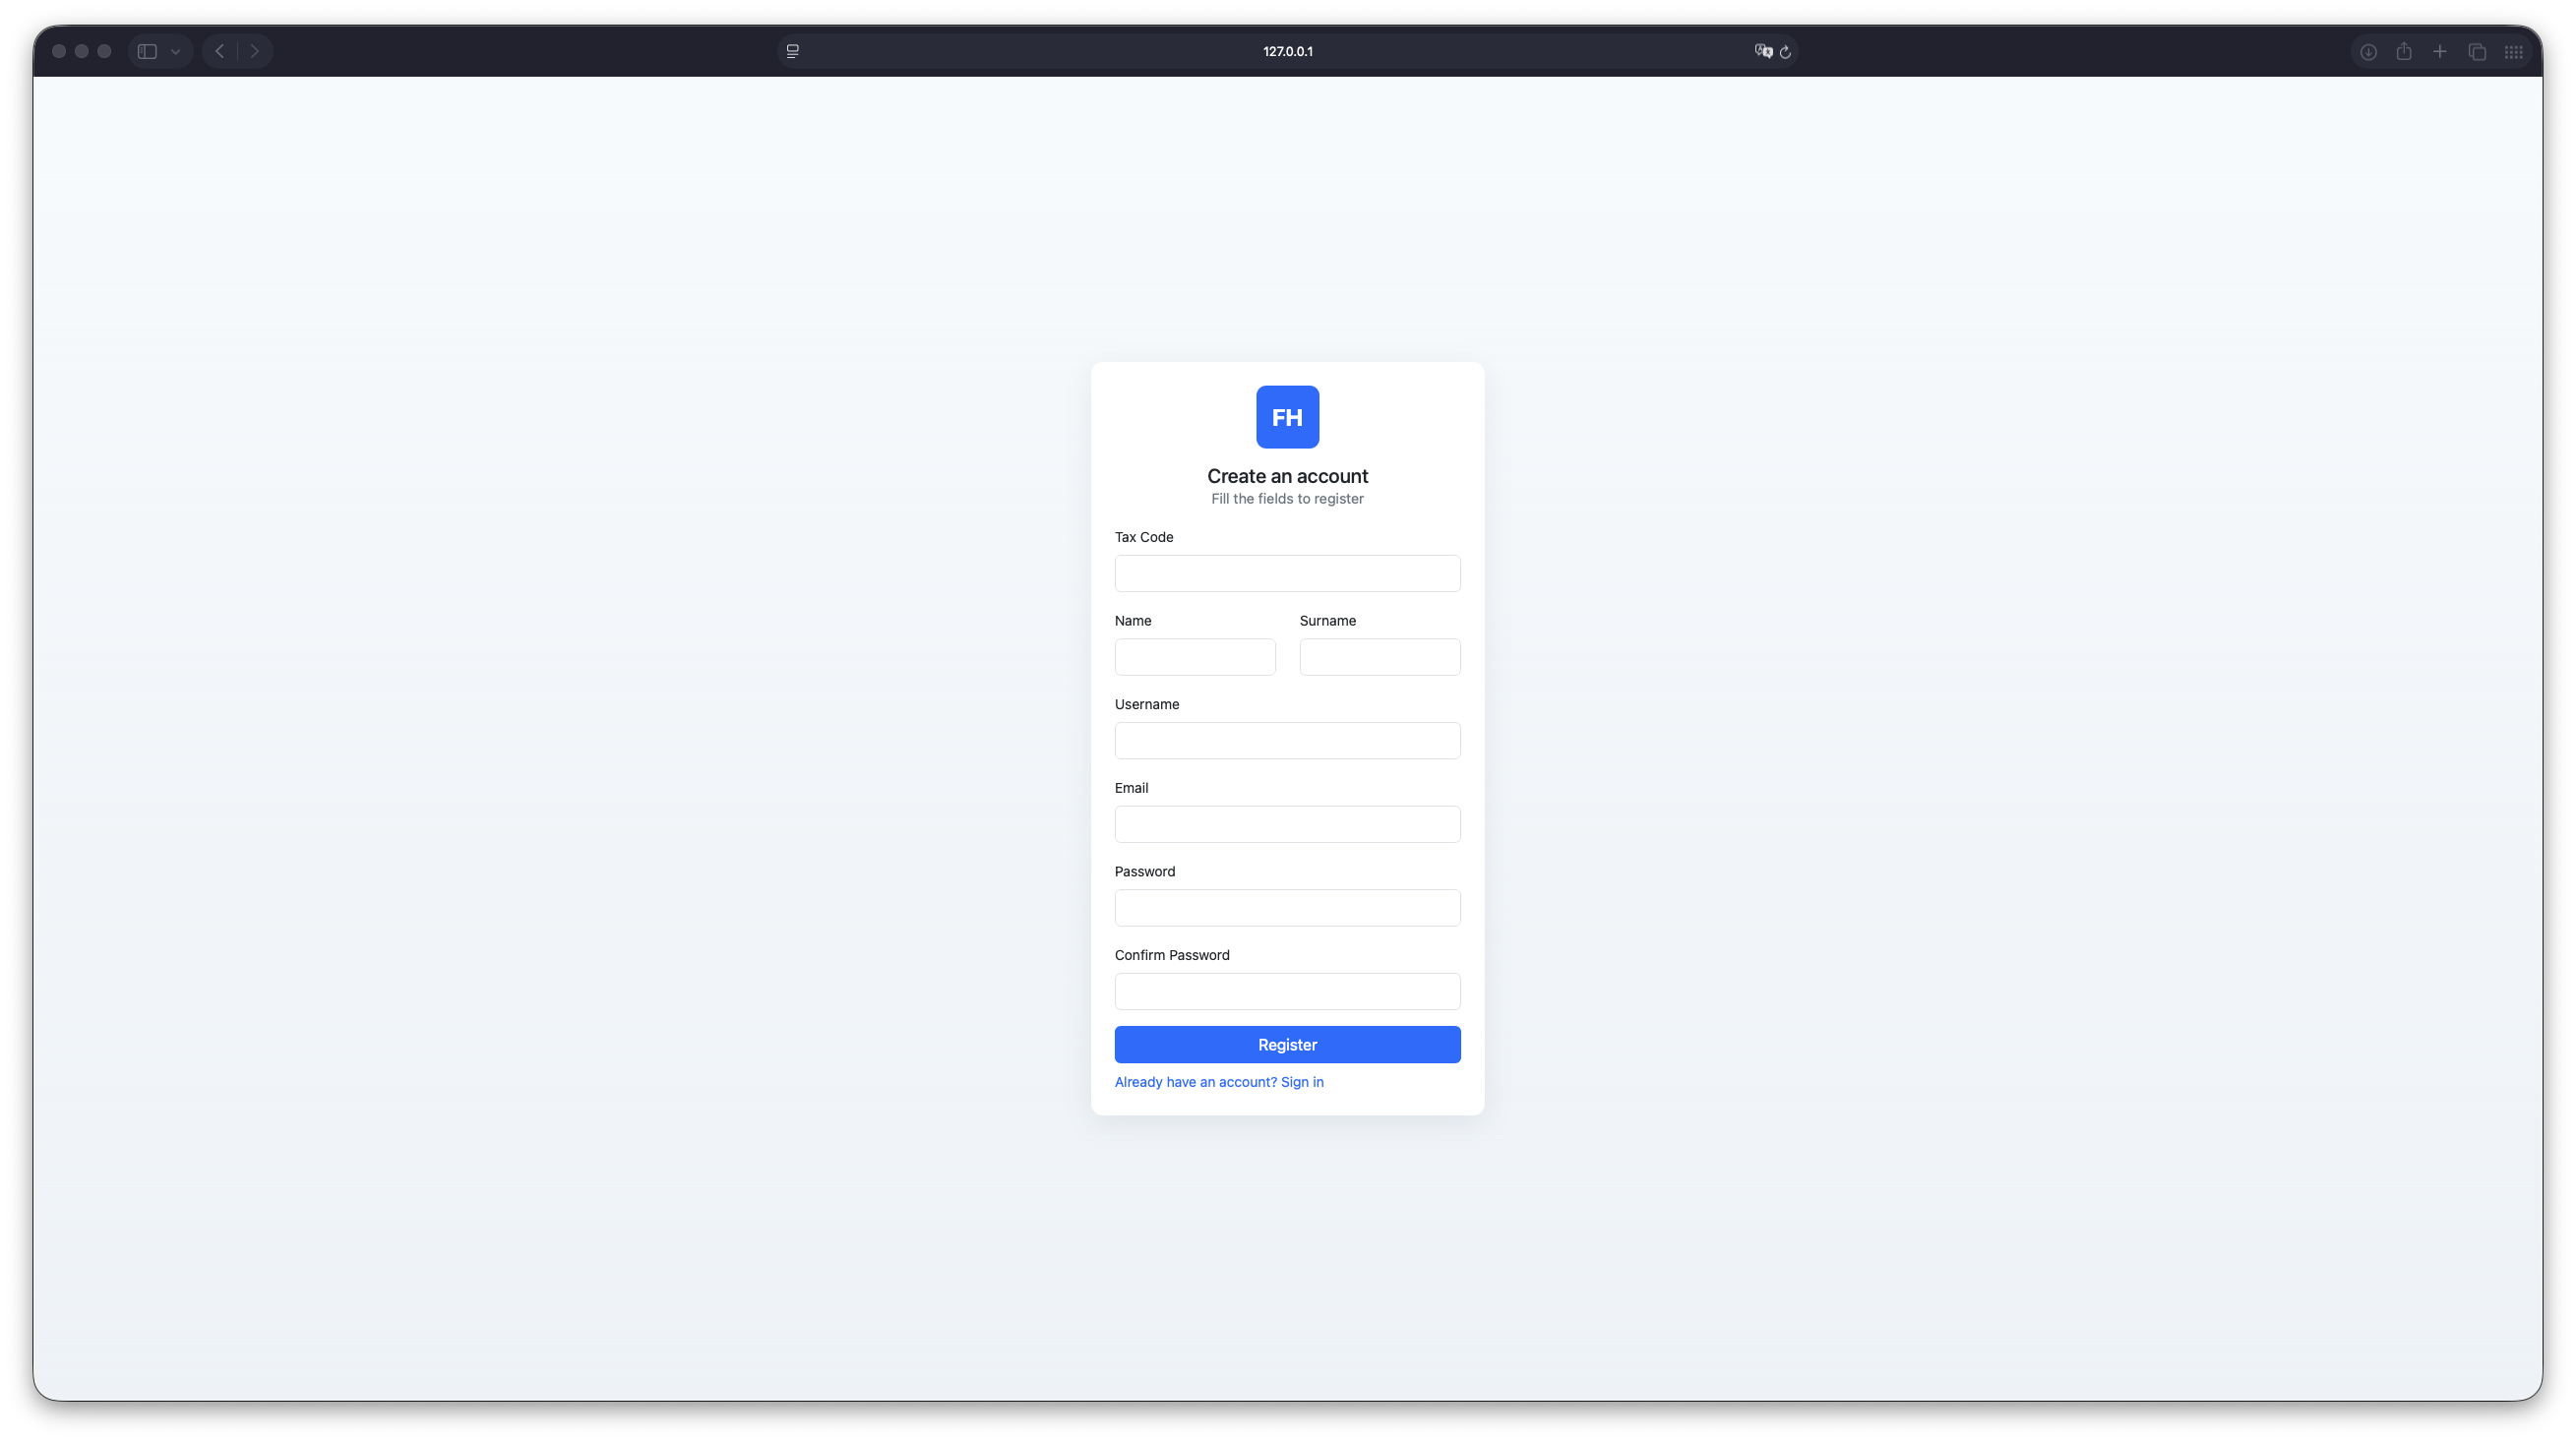
\includegraphics[width=\textwidth, trim=0 0 0 0]{./img/register.png}
  \vspace{-1em}
  \label{fig:registrazione}
\end{figure}

\newpage
\section{Interfaccia Utente}
Dopo l'accesso, l'utente potrà visualizzare il profilo, con le
prenotazioni e gli ordini, con
la possibilità di recensire o annullare prenotazioni future.

\begin{figure}[H]
  \centering
  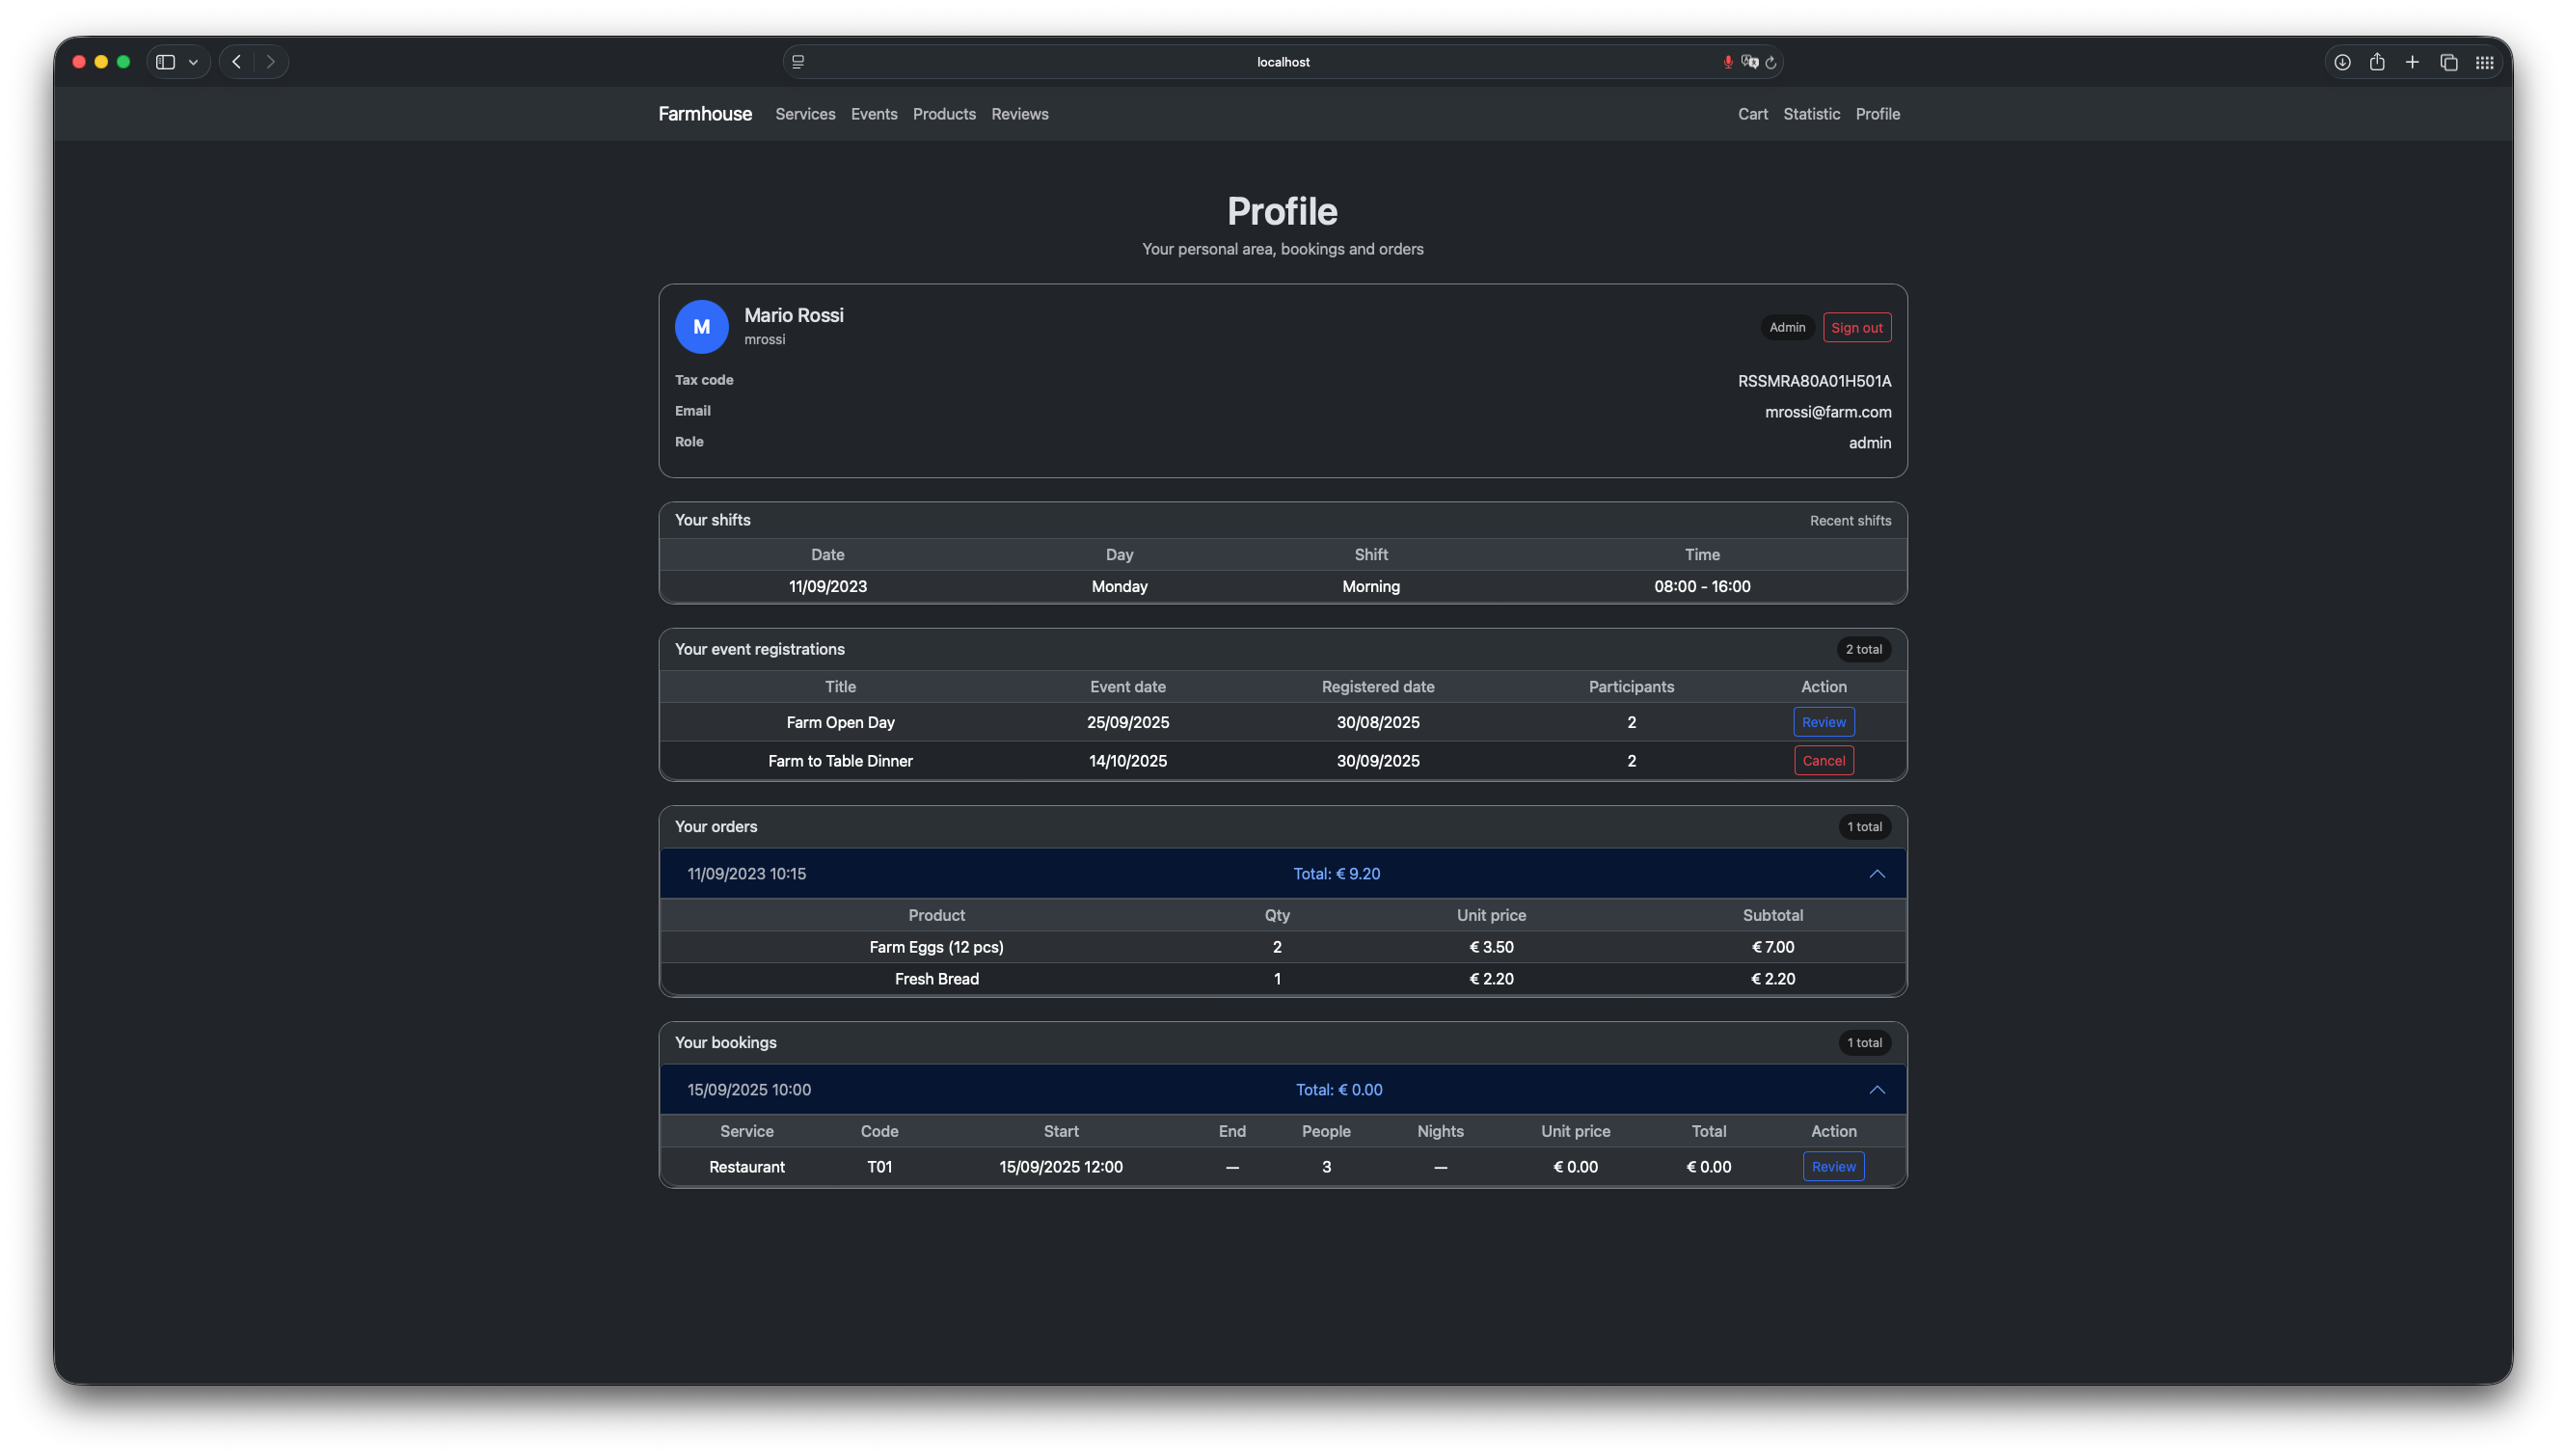
\includegraphics[width=\textwidth, trim=0 0 0 0]{./img/users/profile.png}
  \vspace{-1em}
  \label{fig:profile}
\end{figure}

\subsection*{Servizi}
Dopo aver scelto il servizio da prenotare, è sufficiente inserire i
dati necessari; il sistema
mostrerà la disponibilità aggiornata del servizio selezionato.

\begin{figure}[H]
  \centering
  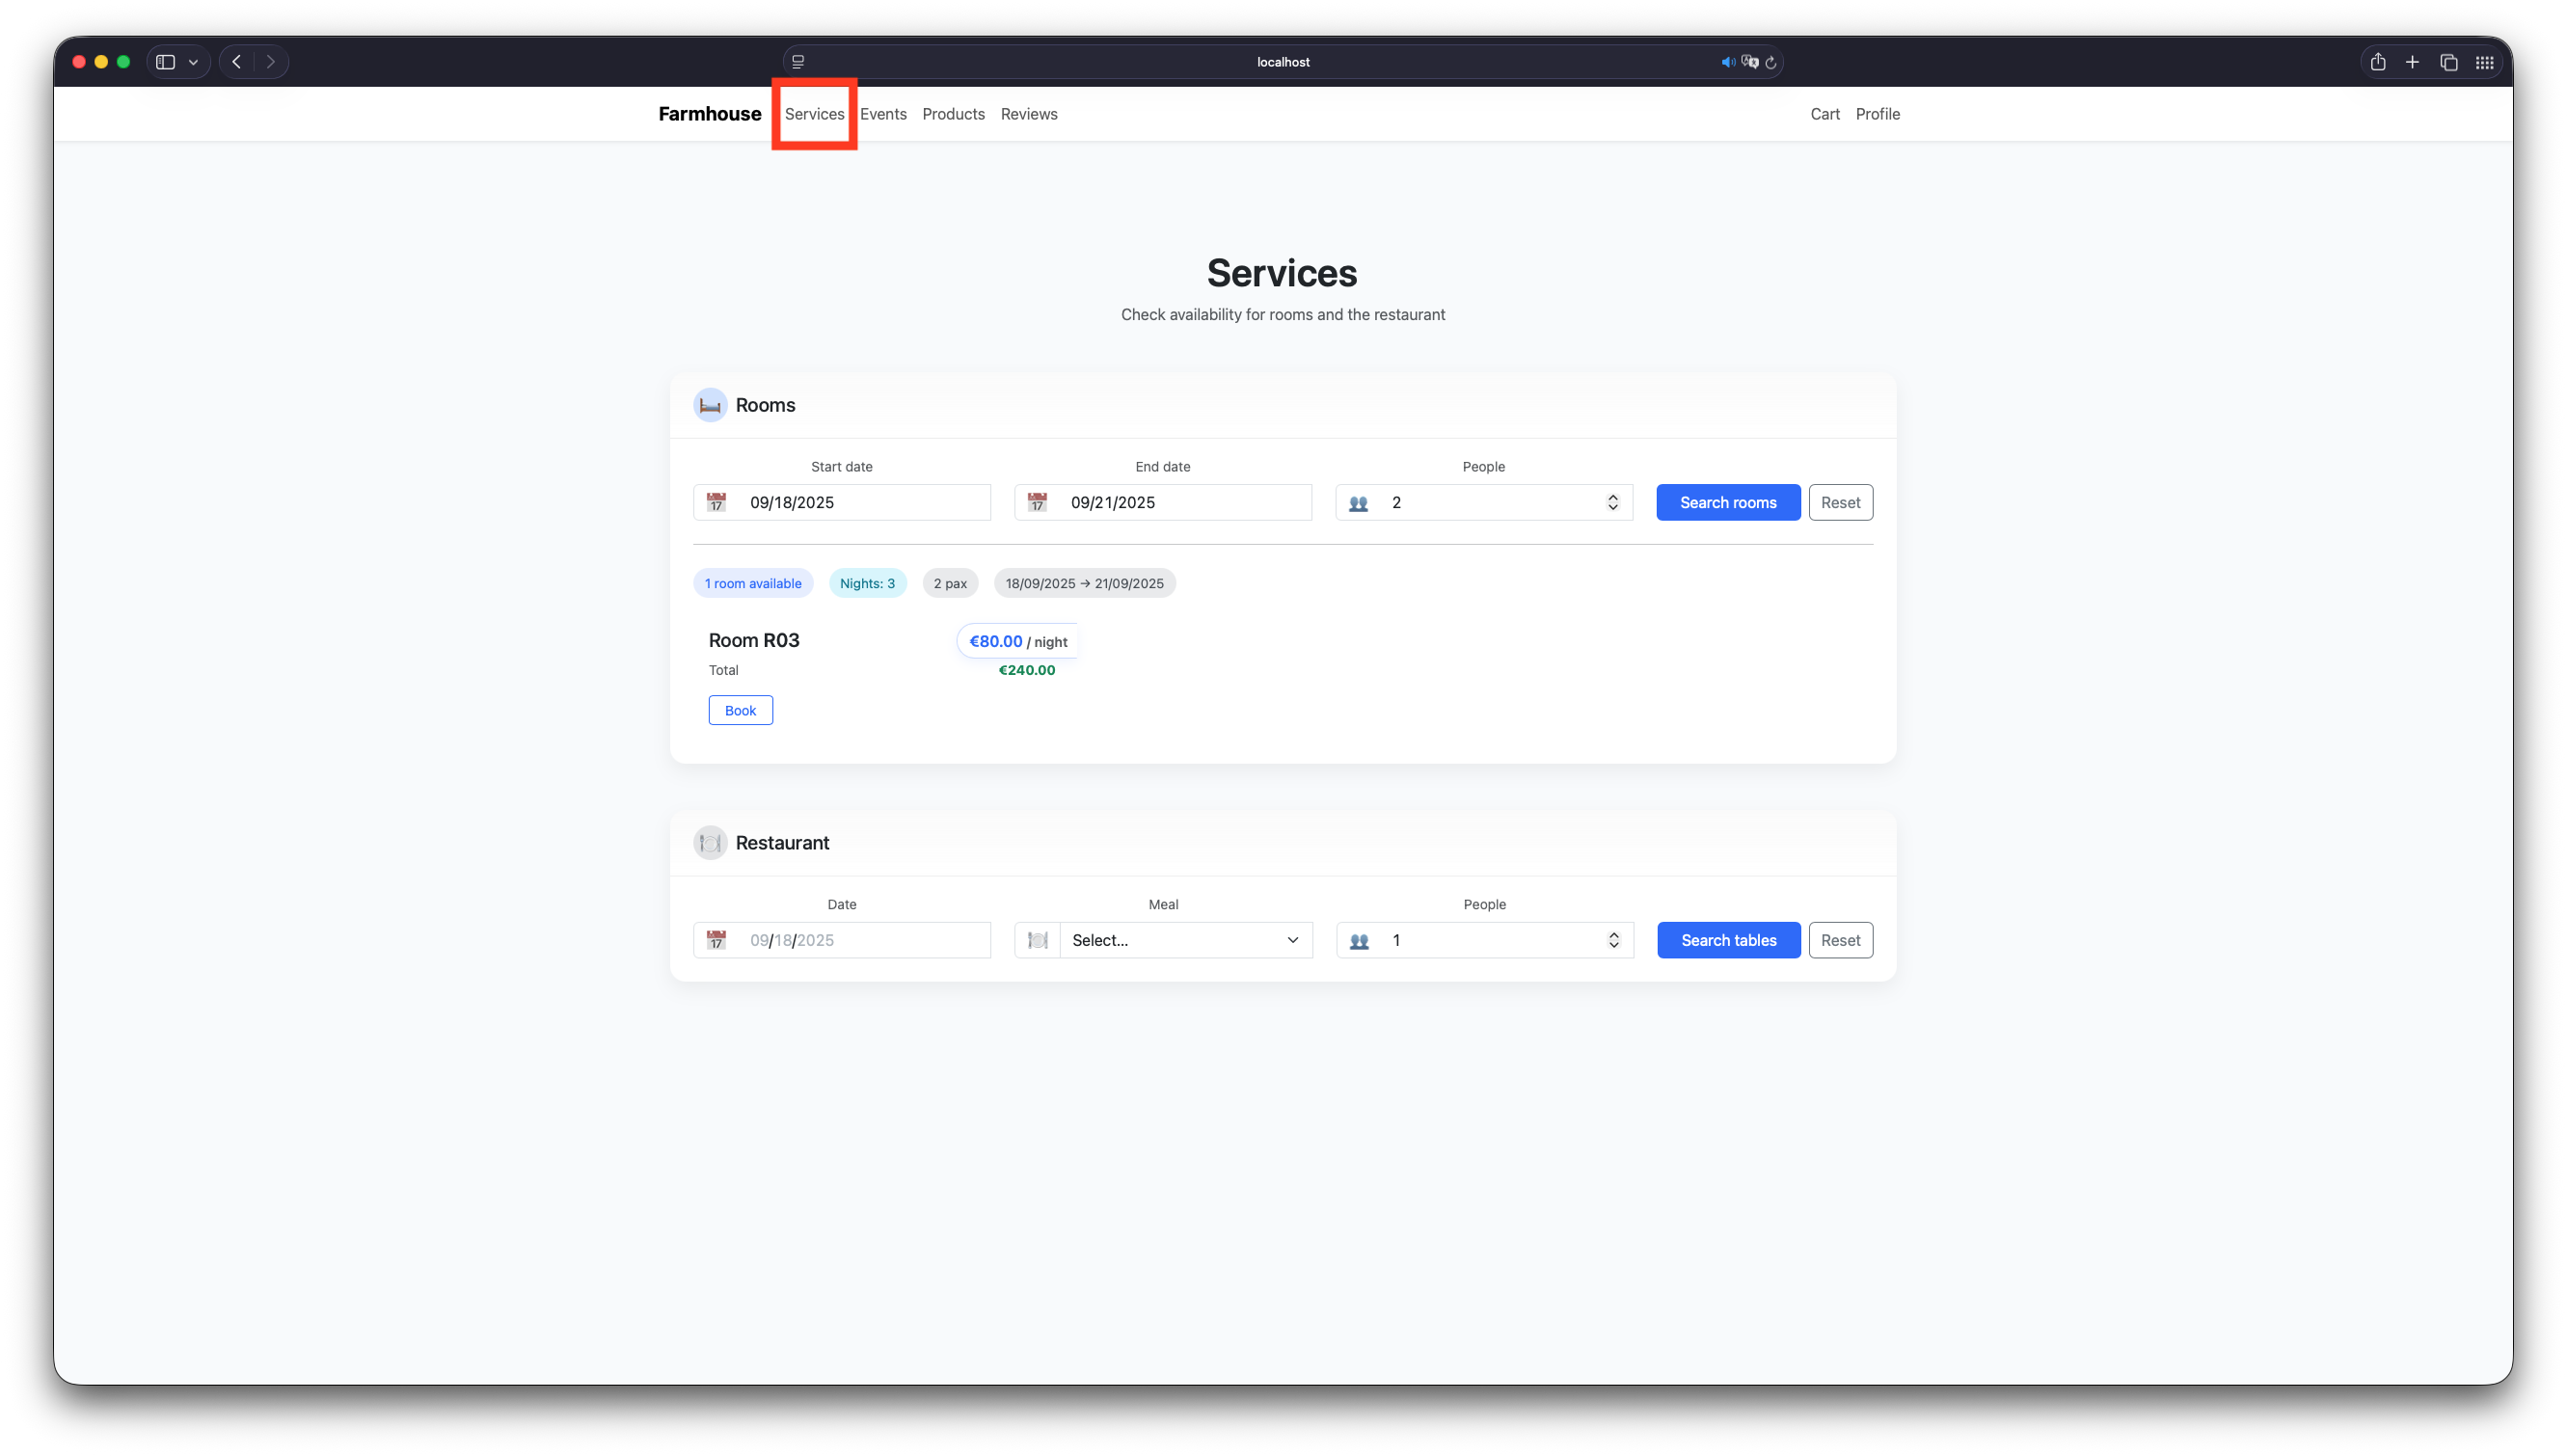
\includegraphics[width=\textwidth, trim=0 0 0 0]{./img/users/services.png}
  \vspace{-1em}
  \label{fig:services}
\end{figure}

\subsection*{Eventi}
Nella sezione eventi, viene mostrato l'elenco degli eventi
disponibili. L'utente può selezionare
l'evento di interesse, specificare il numero di partecipanti e
procedere con la prenotazione.

\begin{figure}[H]
  \centering
  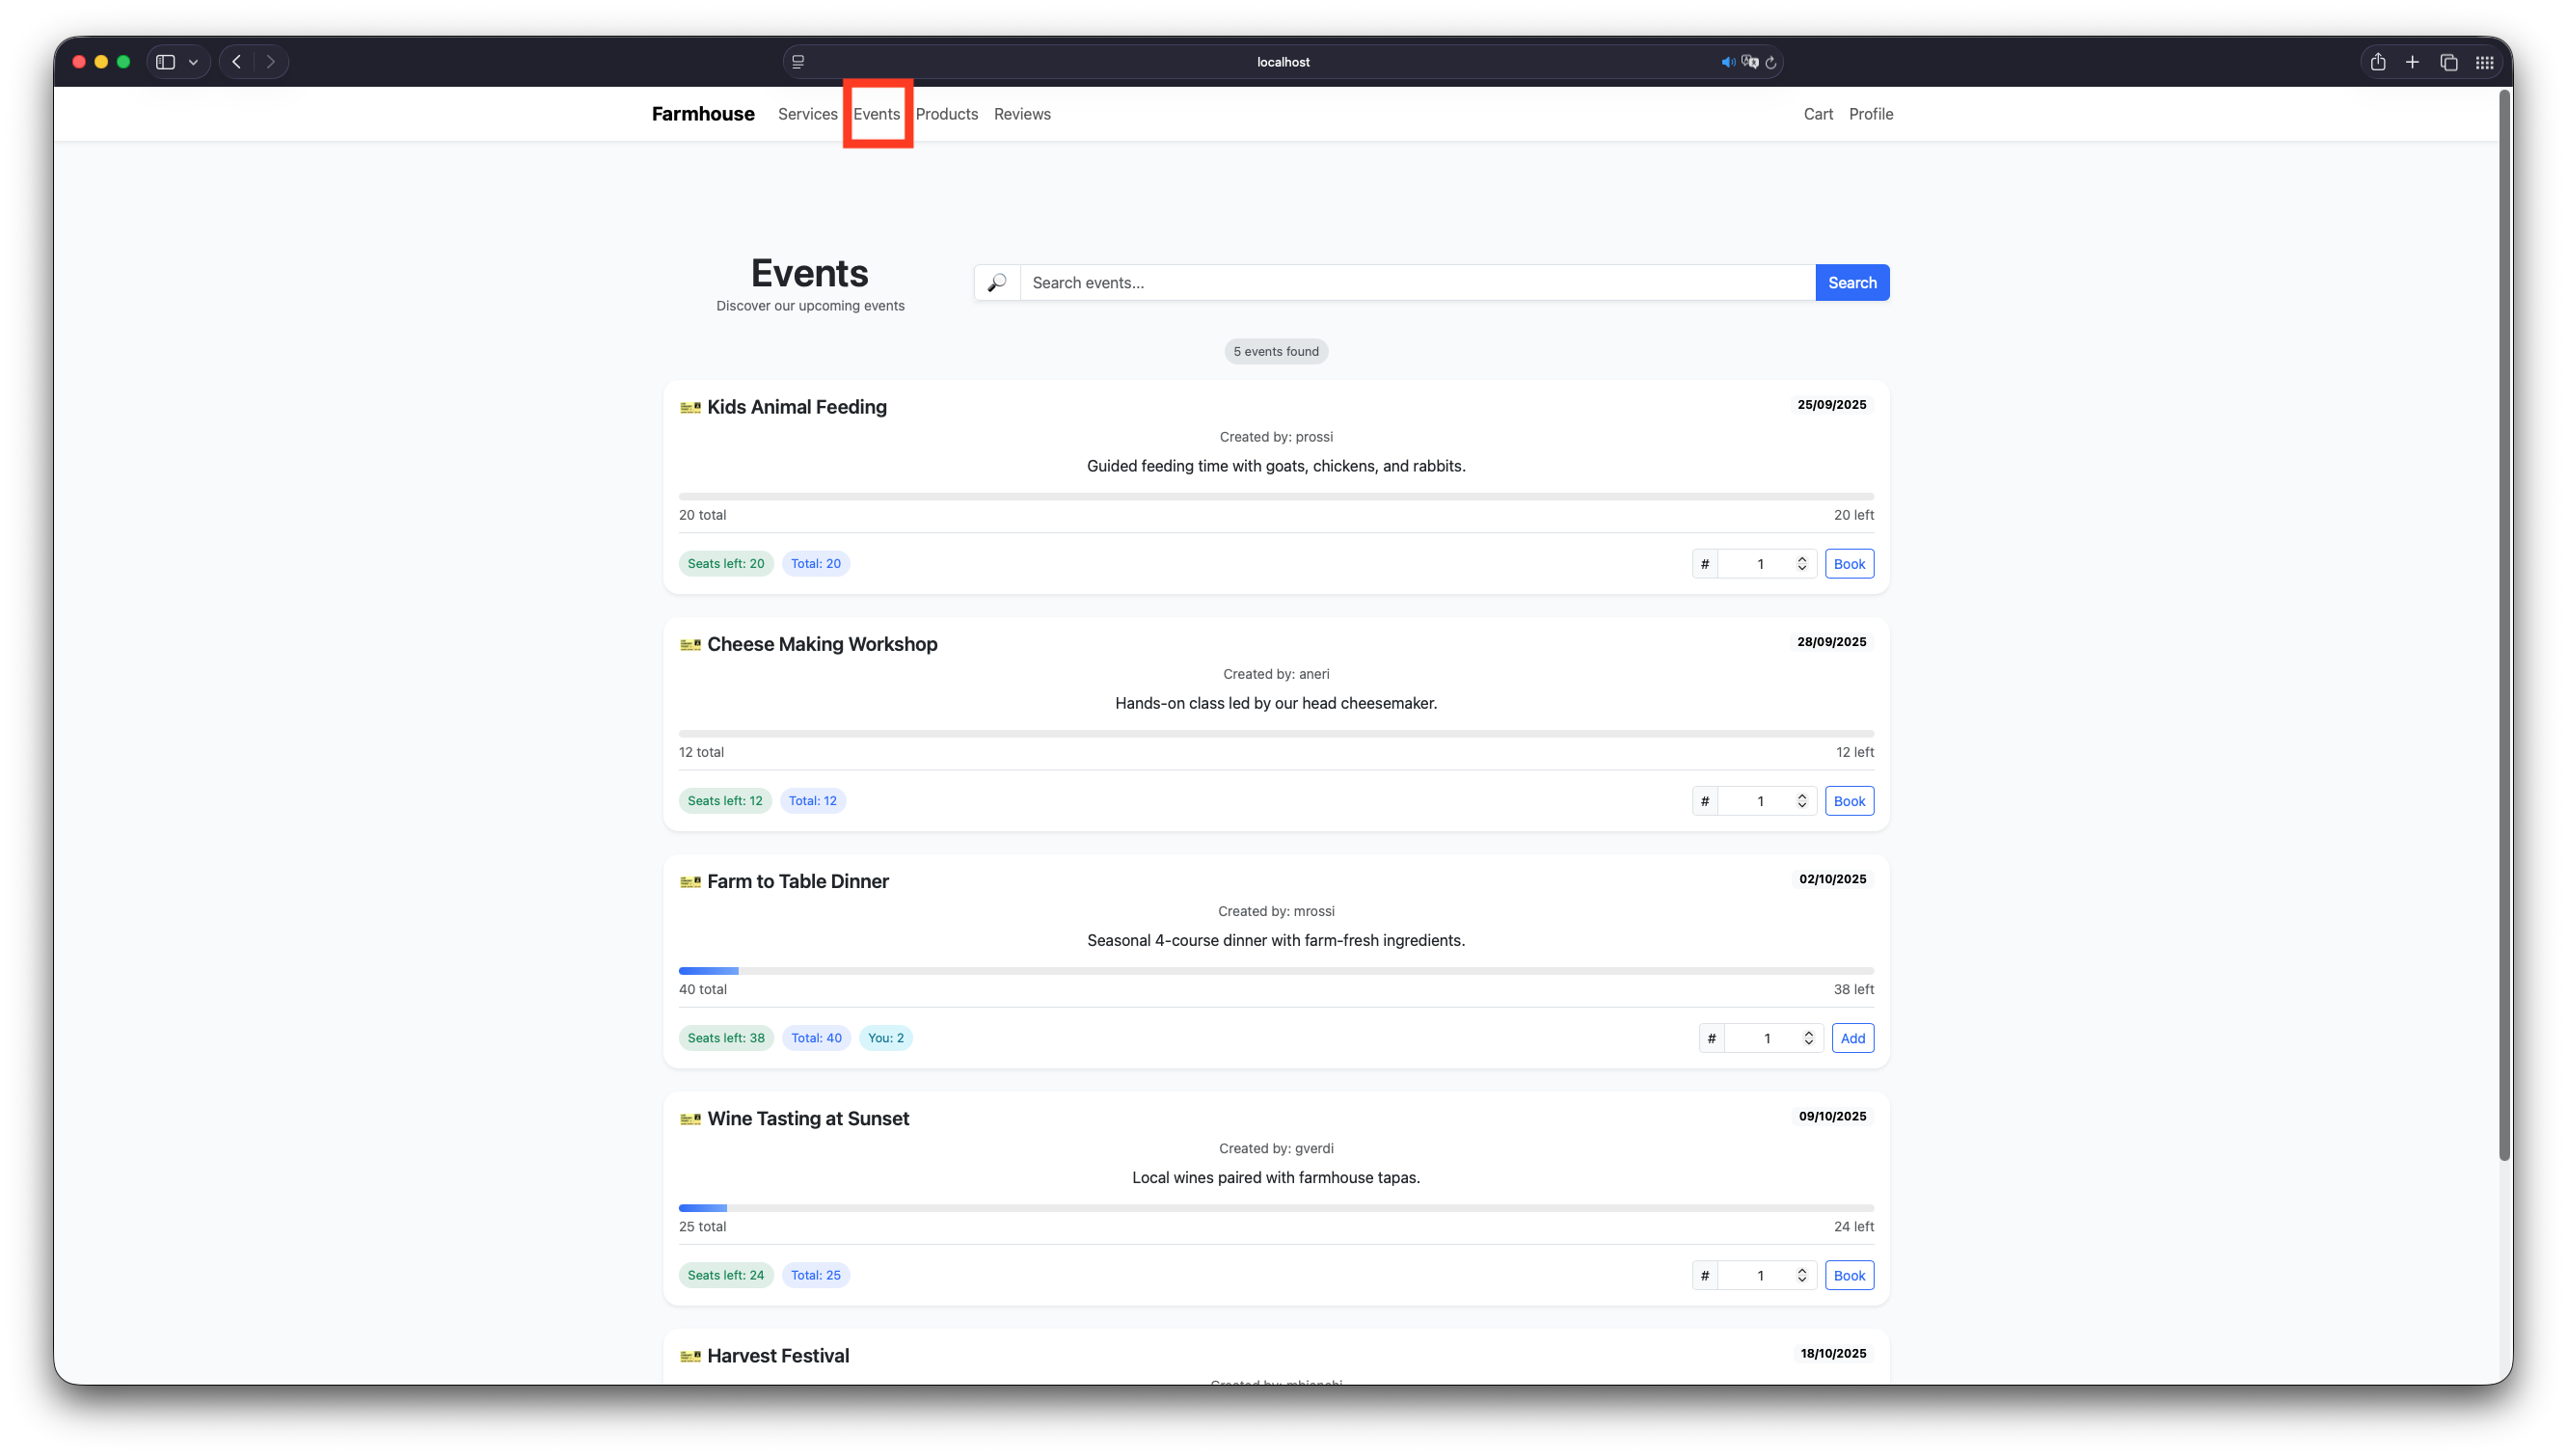
\includegraphics[width=\textwidth, trim=0 0 0 0]{./img/users/events.png}
  \vspace{-1em}
  \label{fig:events}
\end{figure}

\subsection*{Recensioni}
Gli utenti possono visualizzare tutte le recensioni e filtrarle per
evento o servizio.

\begin{figure}[H]
  \centering
  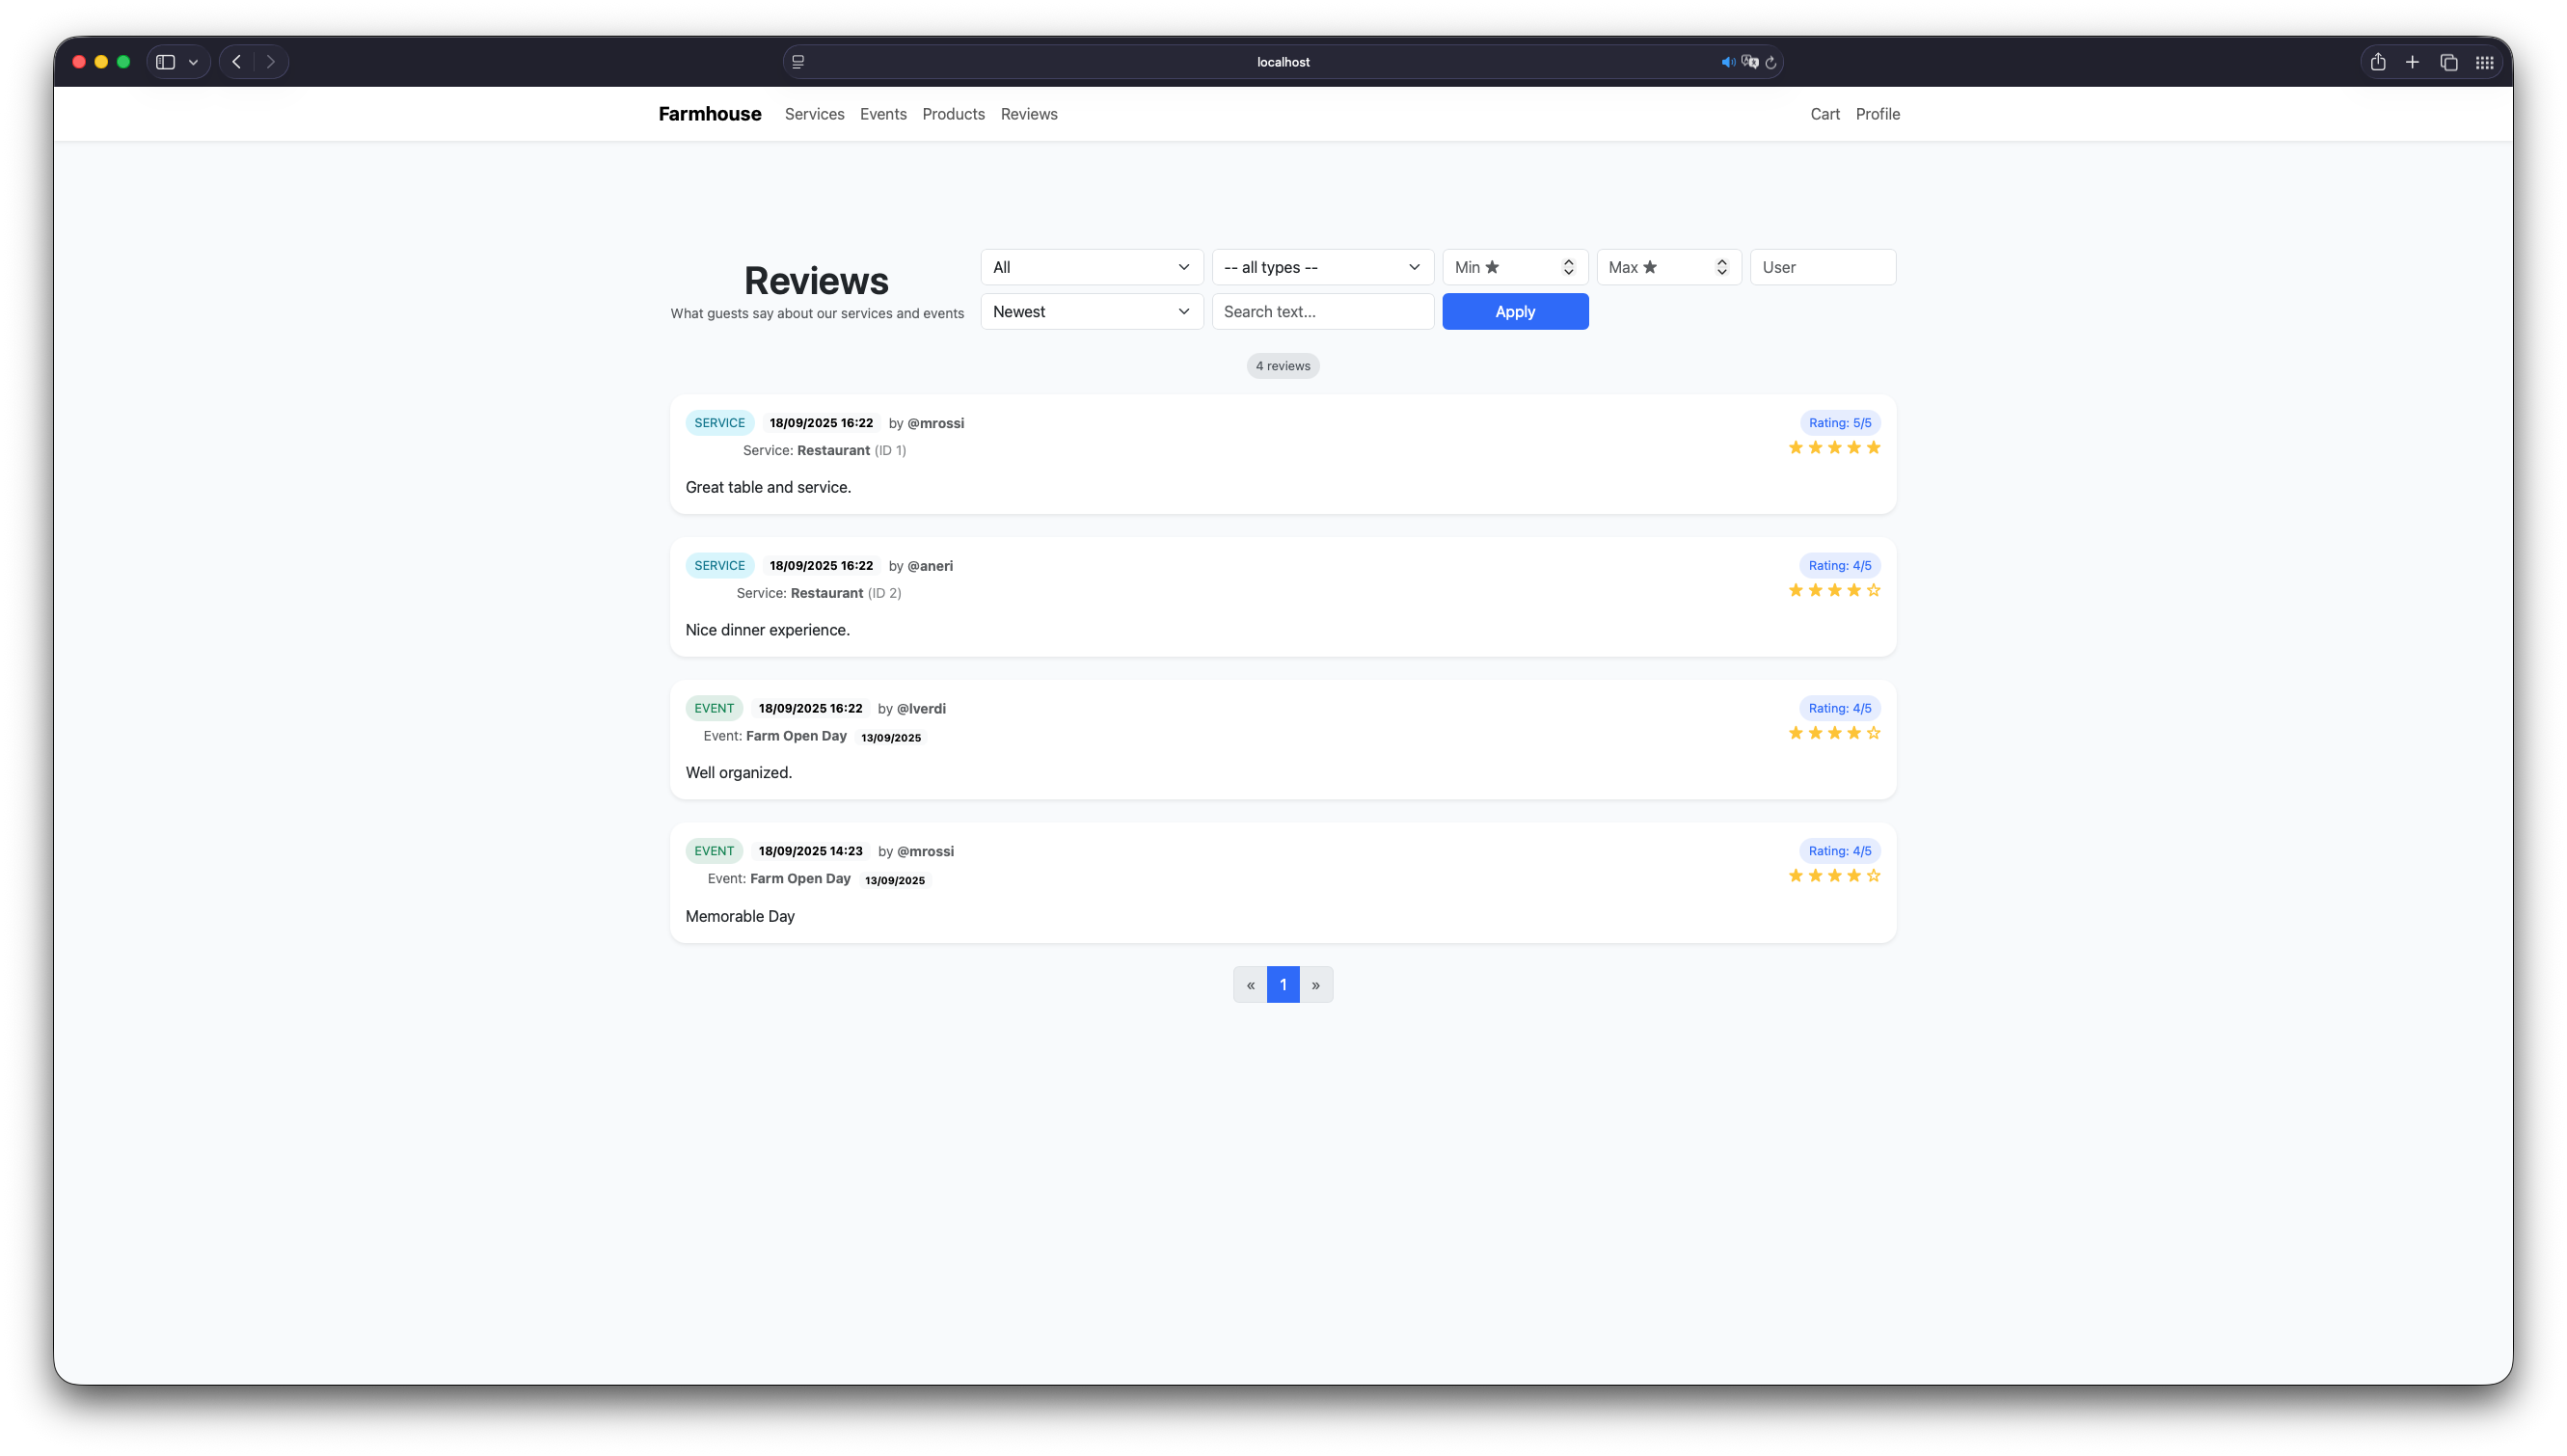
\includegraphics[width=\textwidth, trim=0 0 0 0]{./img/users/reviews.png}
  \vspace{-1em}
  \label{fig:recensione}
\end{figure}

Il form permette agli utenti di lasciare una recensione su eventi o
servizi a cui hanno partecipato,
inserendo commento e voto. La recensione è consentita solo dopo la
partecipazione effettiva.

\begin{figure}[H]
  \centering
  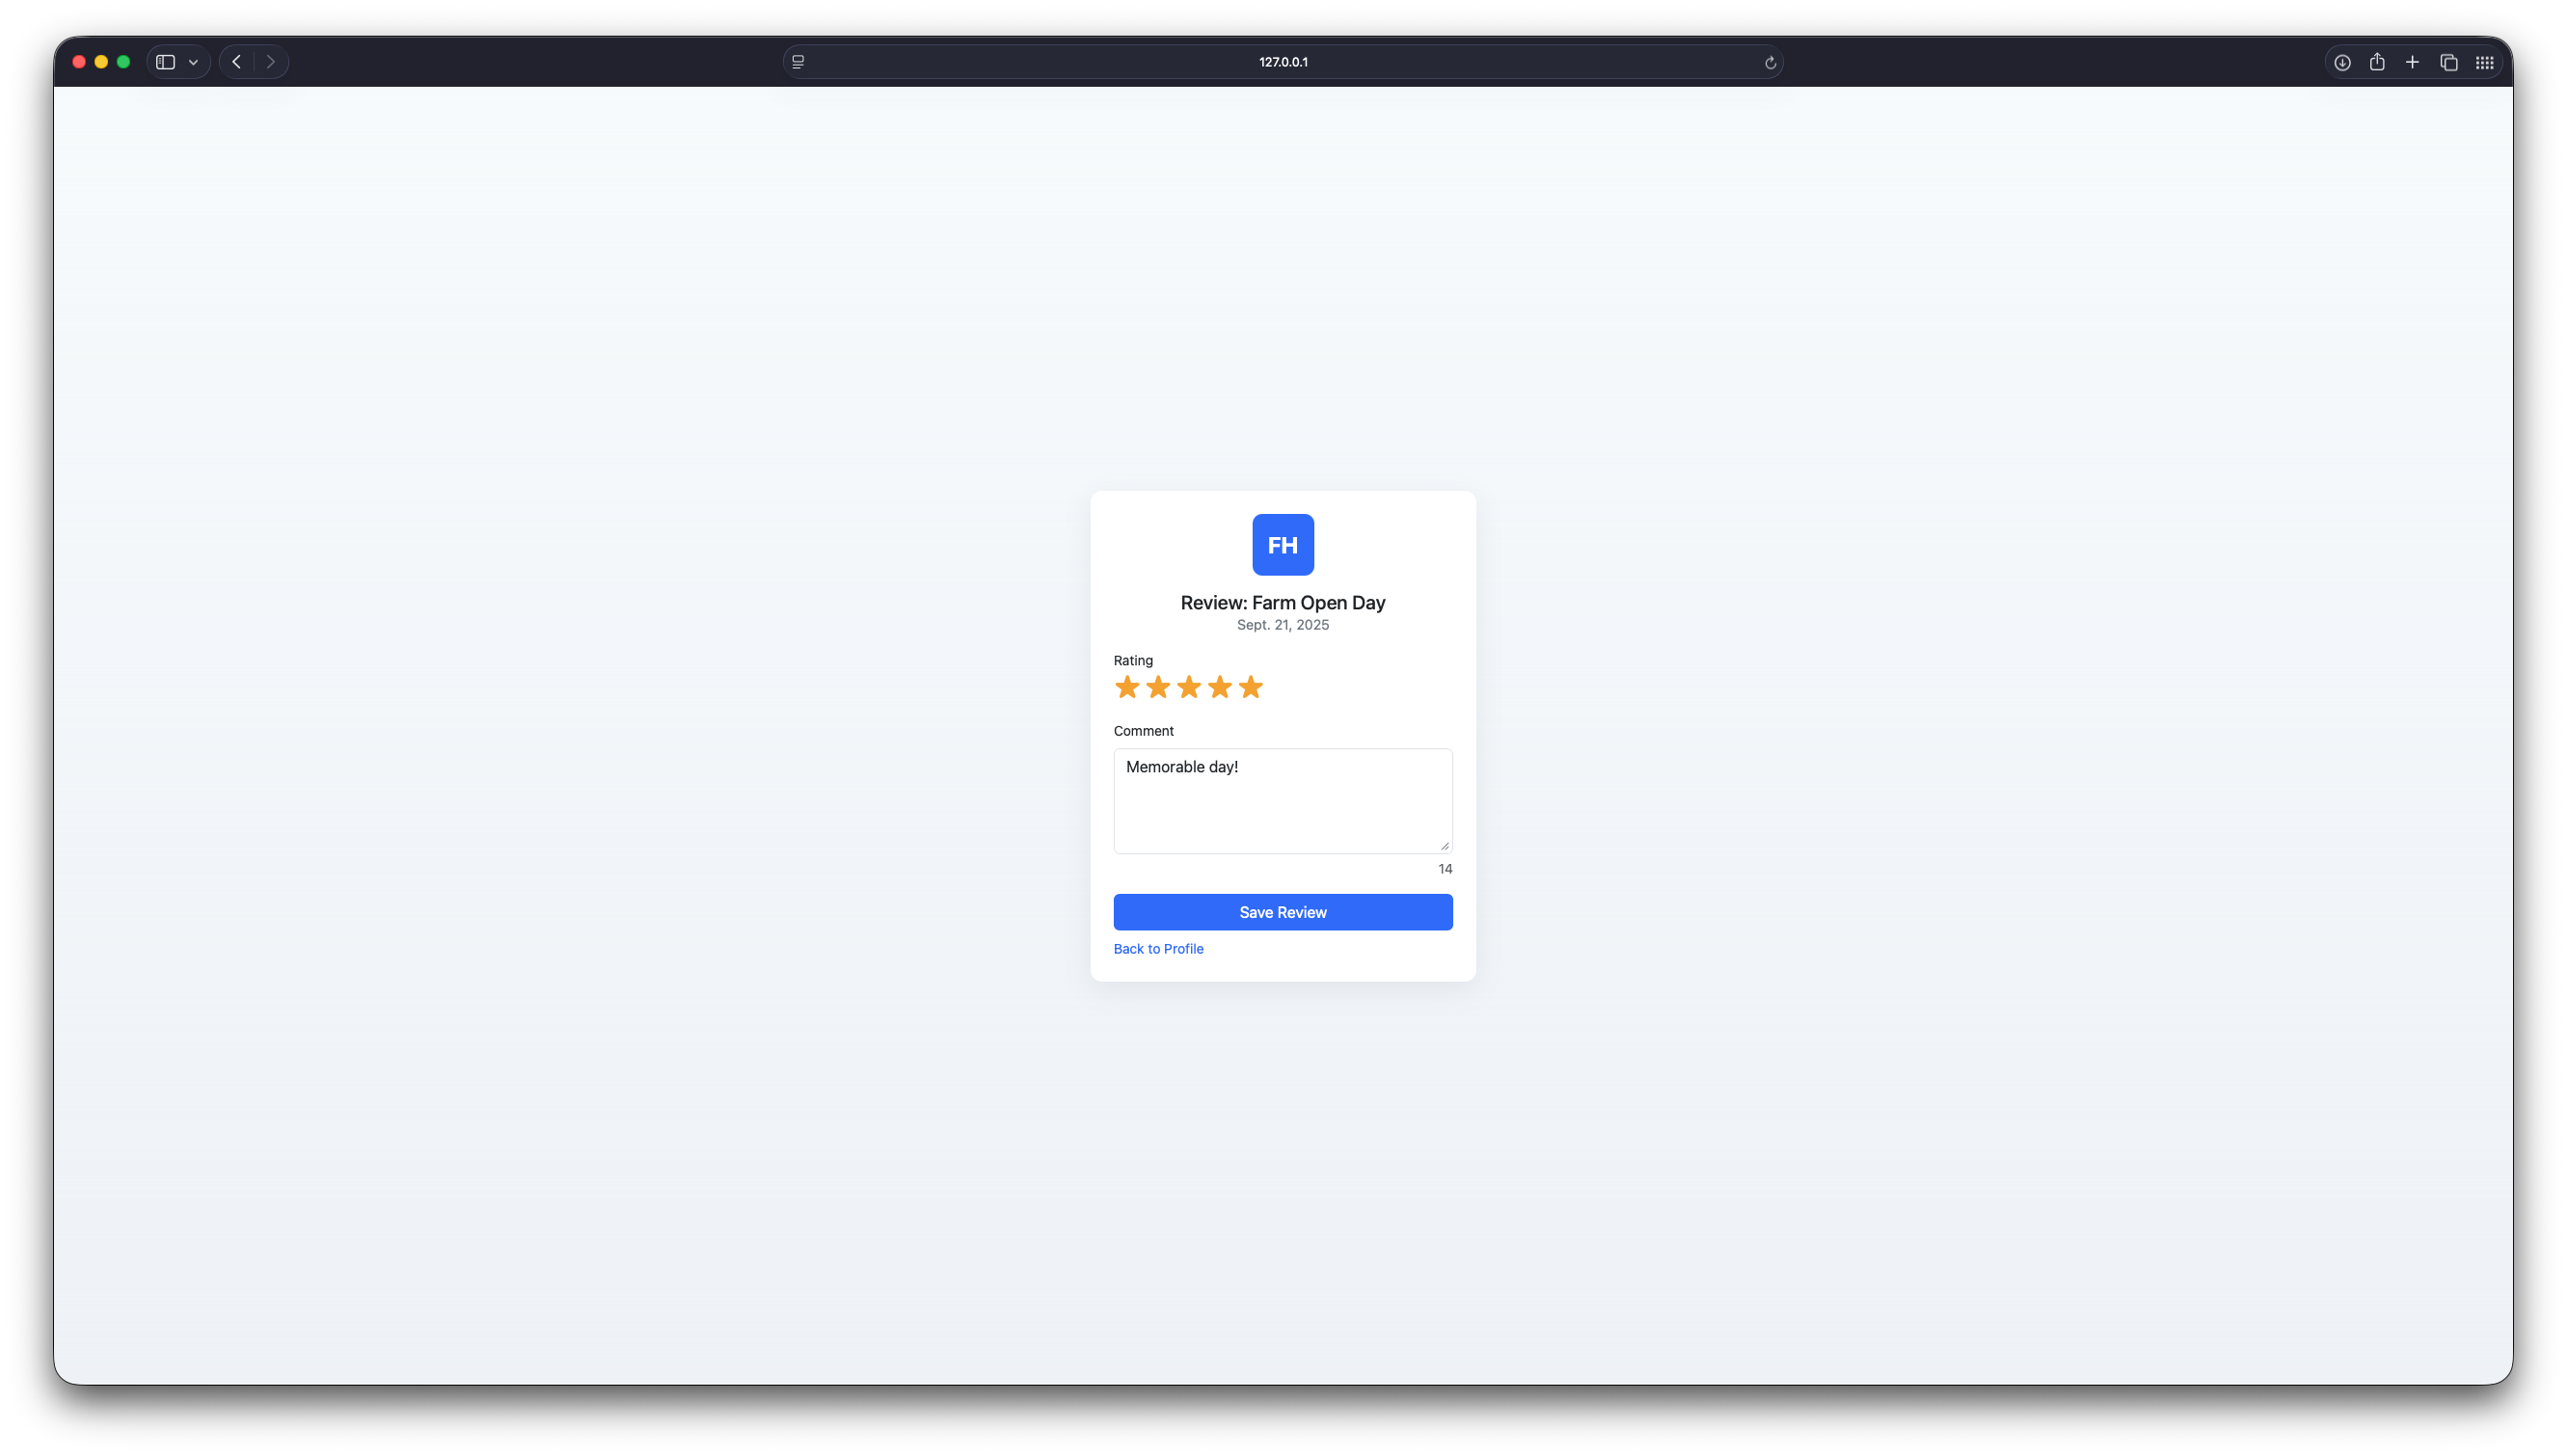
\includegraphics[width=\textwidth, trim=0 0 0 0]{./img/users/give_review.png}
  \vspace{-1em}
  \label{fig:lascia recensione}
\end{figure}

\subsection*{Prodotti}
La sezione prodotti consente agli utenti di consultare il catalogo
aggiungerli al carrello per
l'acquisto. Il sistema mostra in tempo reale il contenuto del
carrello e il totale dell'ordine.
Fatto il checkout sarà visibile il riepilogo nella sezione profilo.

\begin{figure}[H]
  \centering
  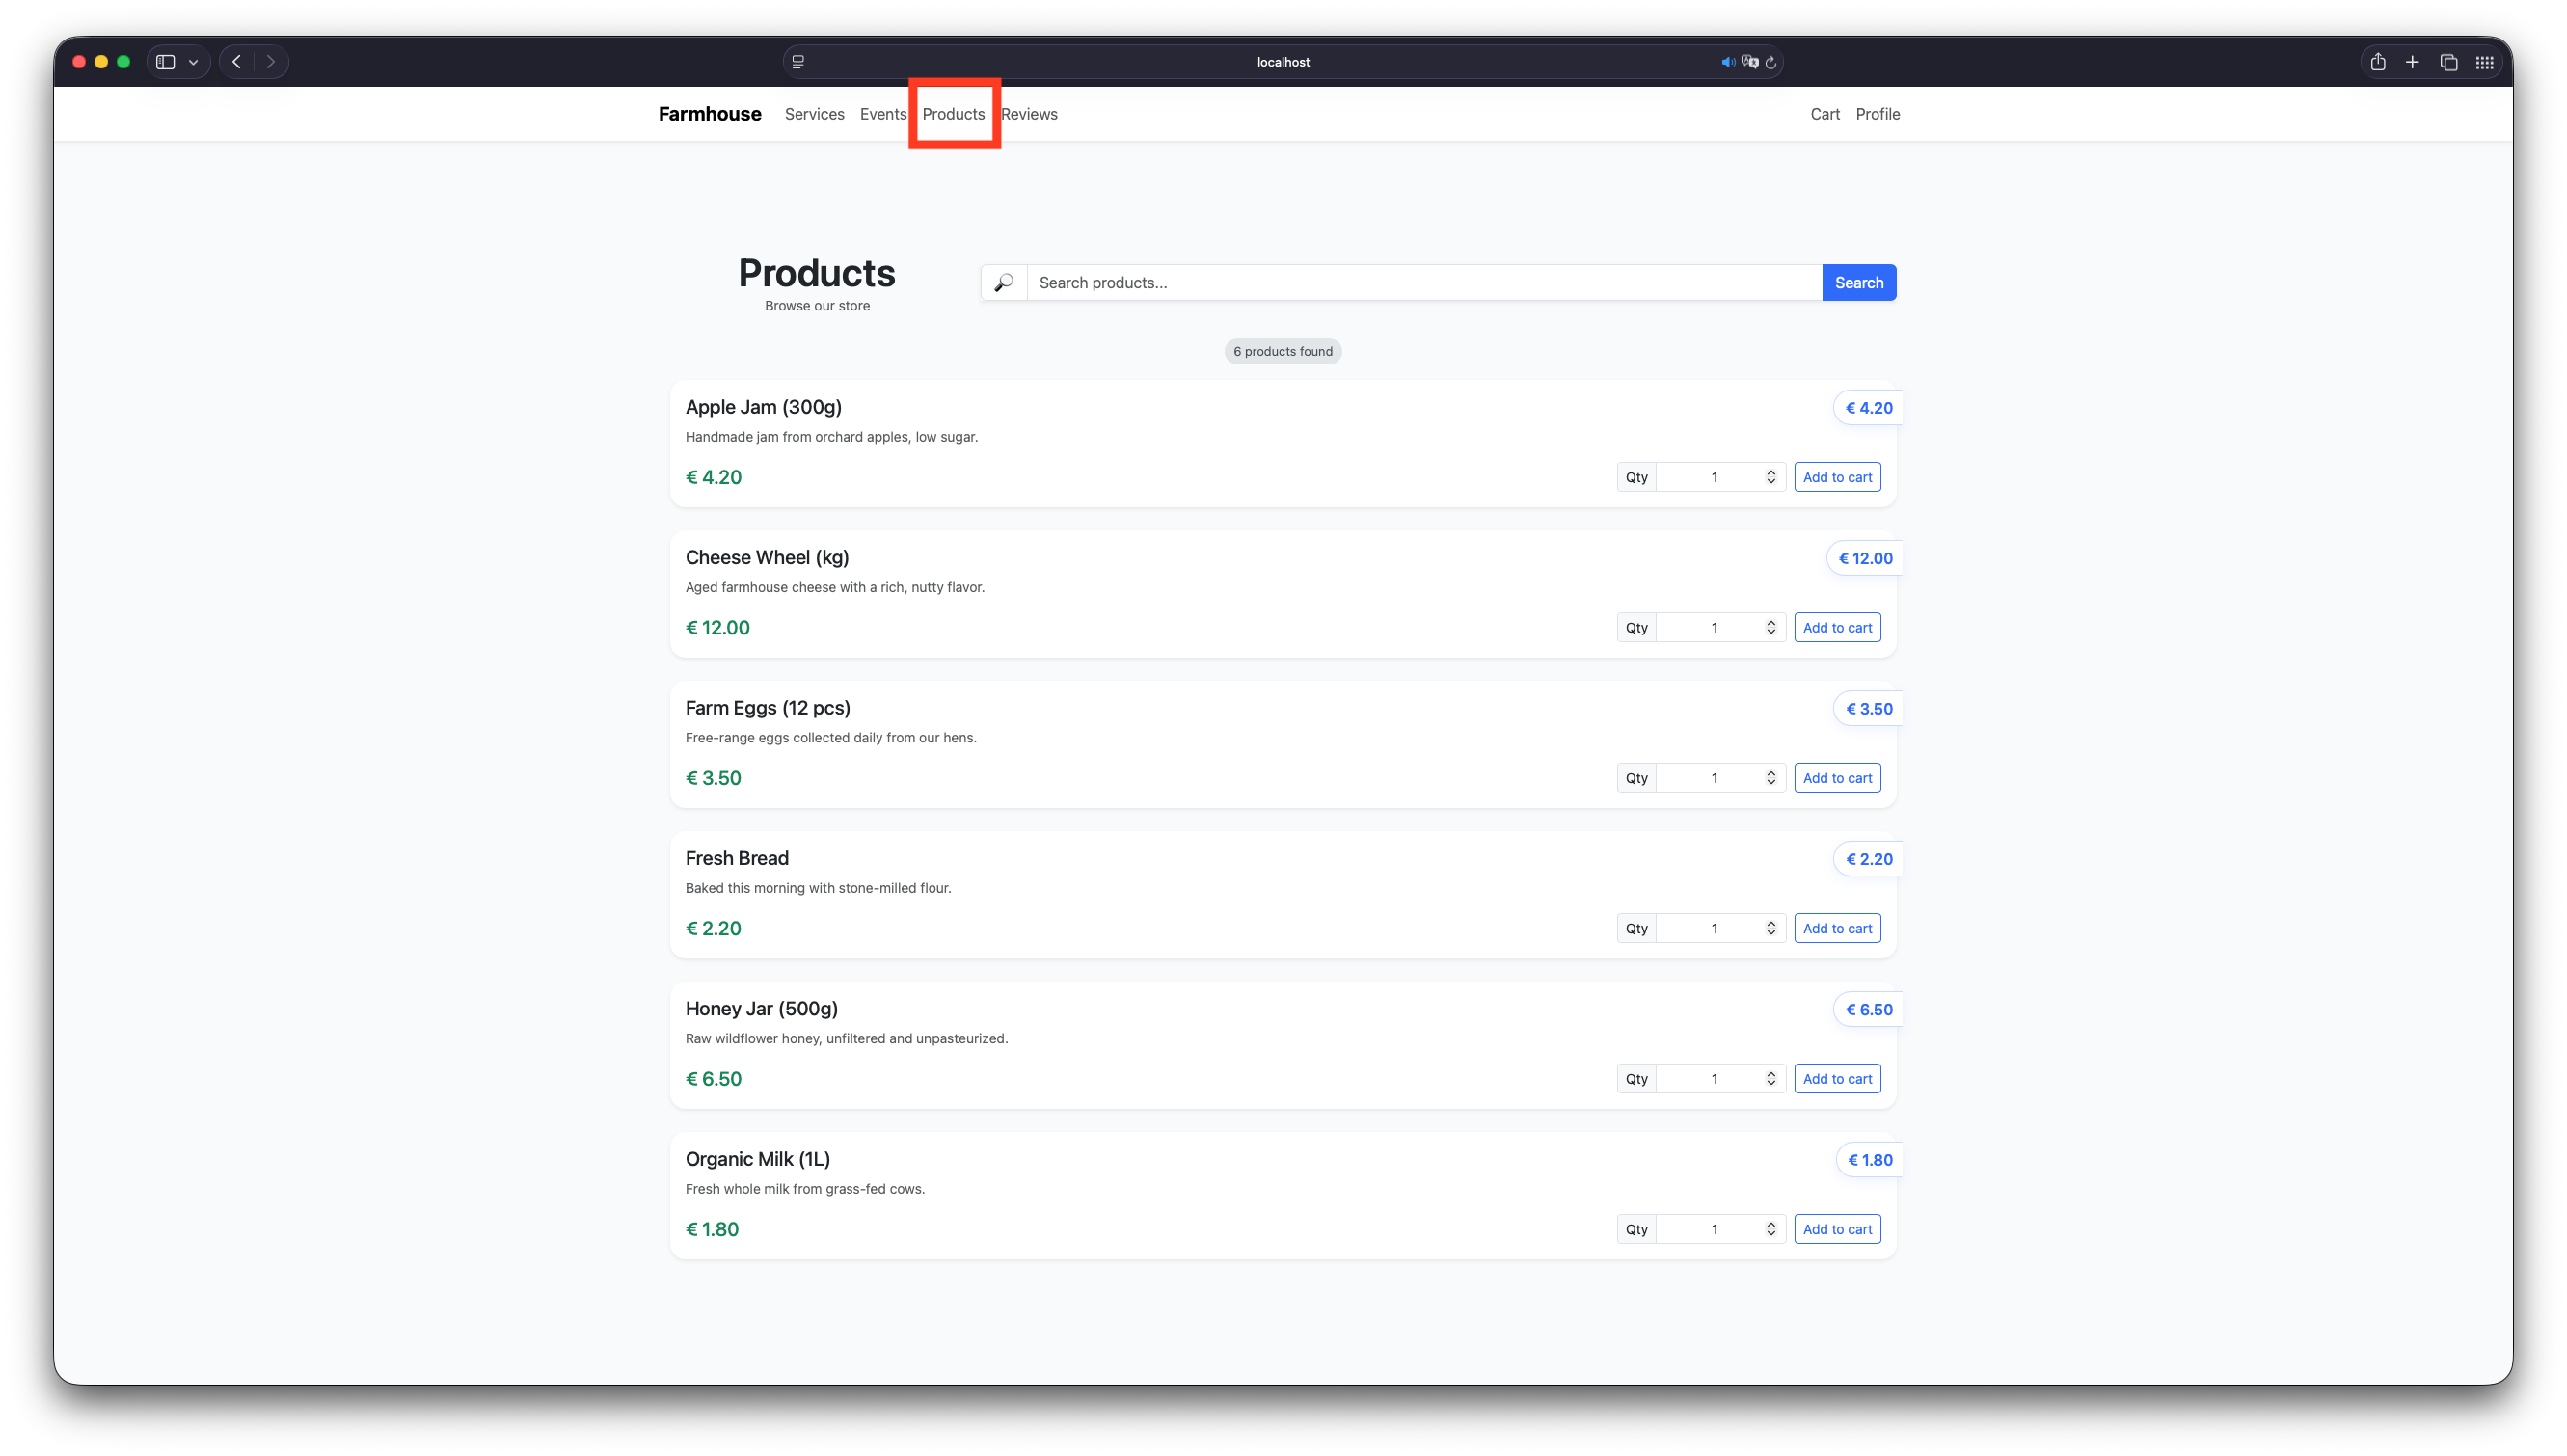
\includegraphics[width=\textwidth, trim=0 0 0 0]{./img/users/products.png}
  \vspace{-1em}
  \label{fig:products}
\end{figure}

\subsection*{Carrello}
Il \textbf{carrello} è una funzionalità applicativa che consente agli
utenti di selezionare e
gestire i prodotti da acquistare prima di confermare l'ordine. Il
carrello non è rappresentato
nel database, ma viene gestito lato applicazione: i prodotti
selezionati vengono memorizzati
temporaneamente fino al checkout, momento in cui viene creato
l'ordine definitivo e
registrato nel sistema.

\begin{figure}[H]
  \centering
  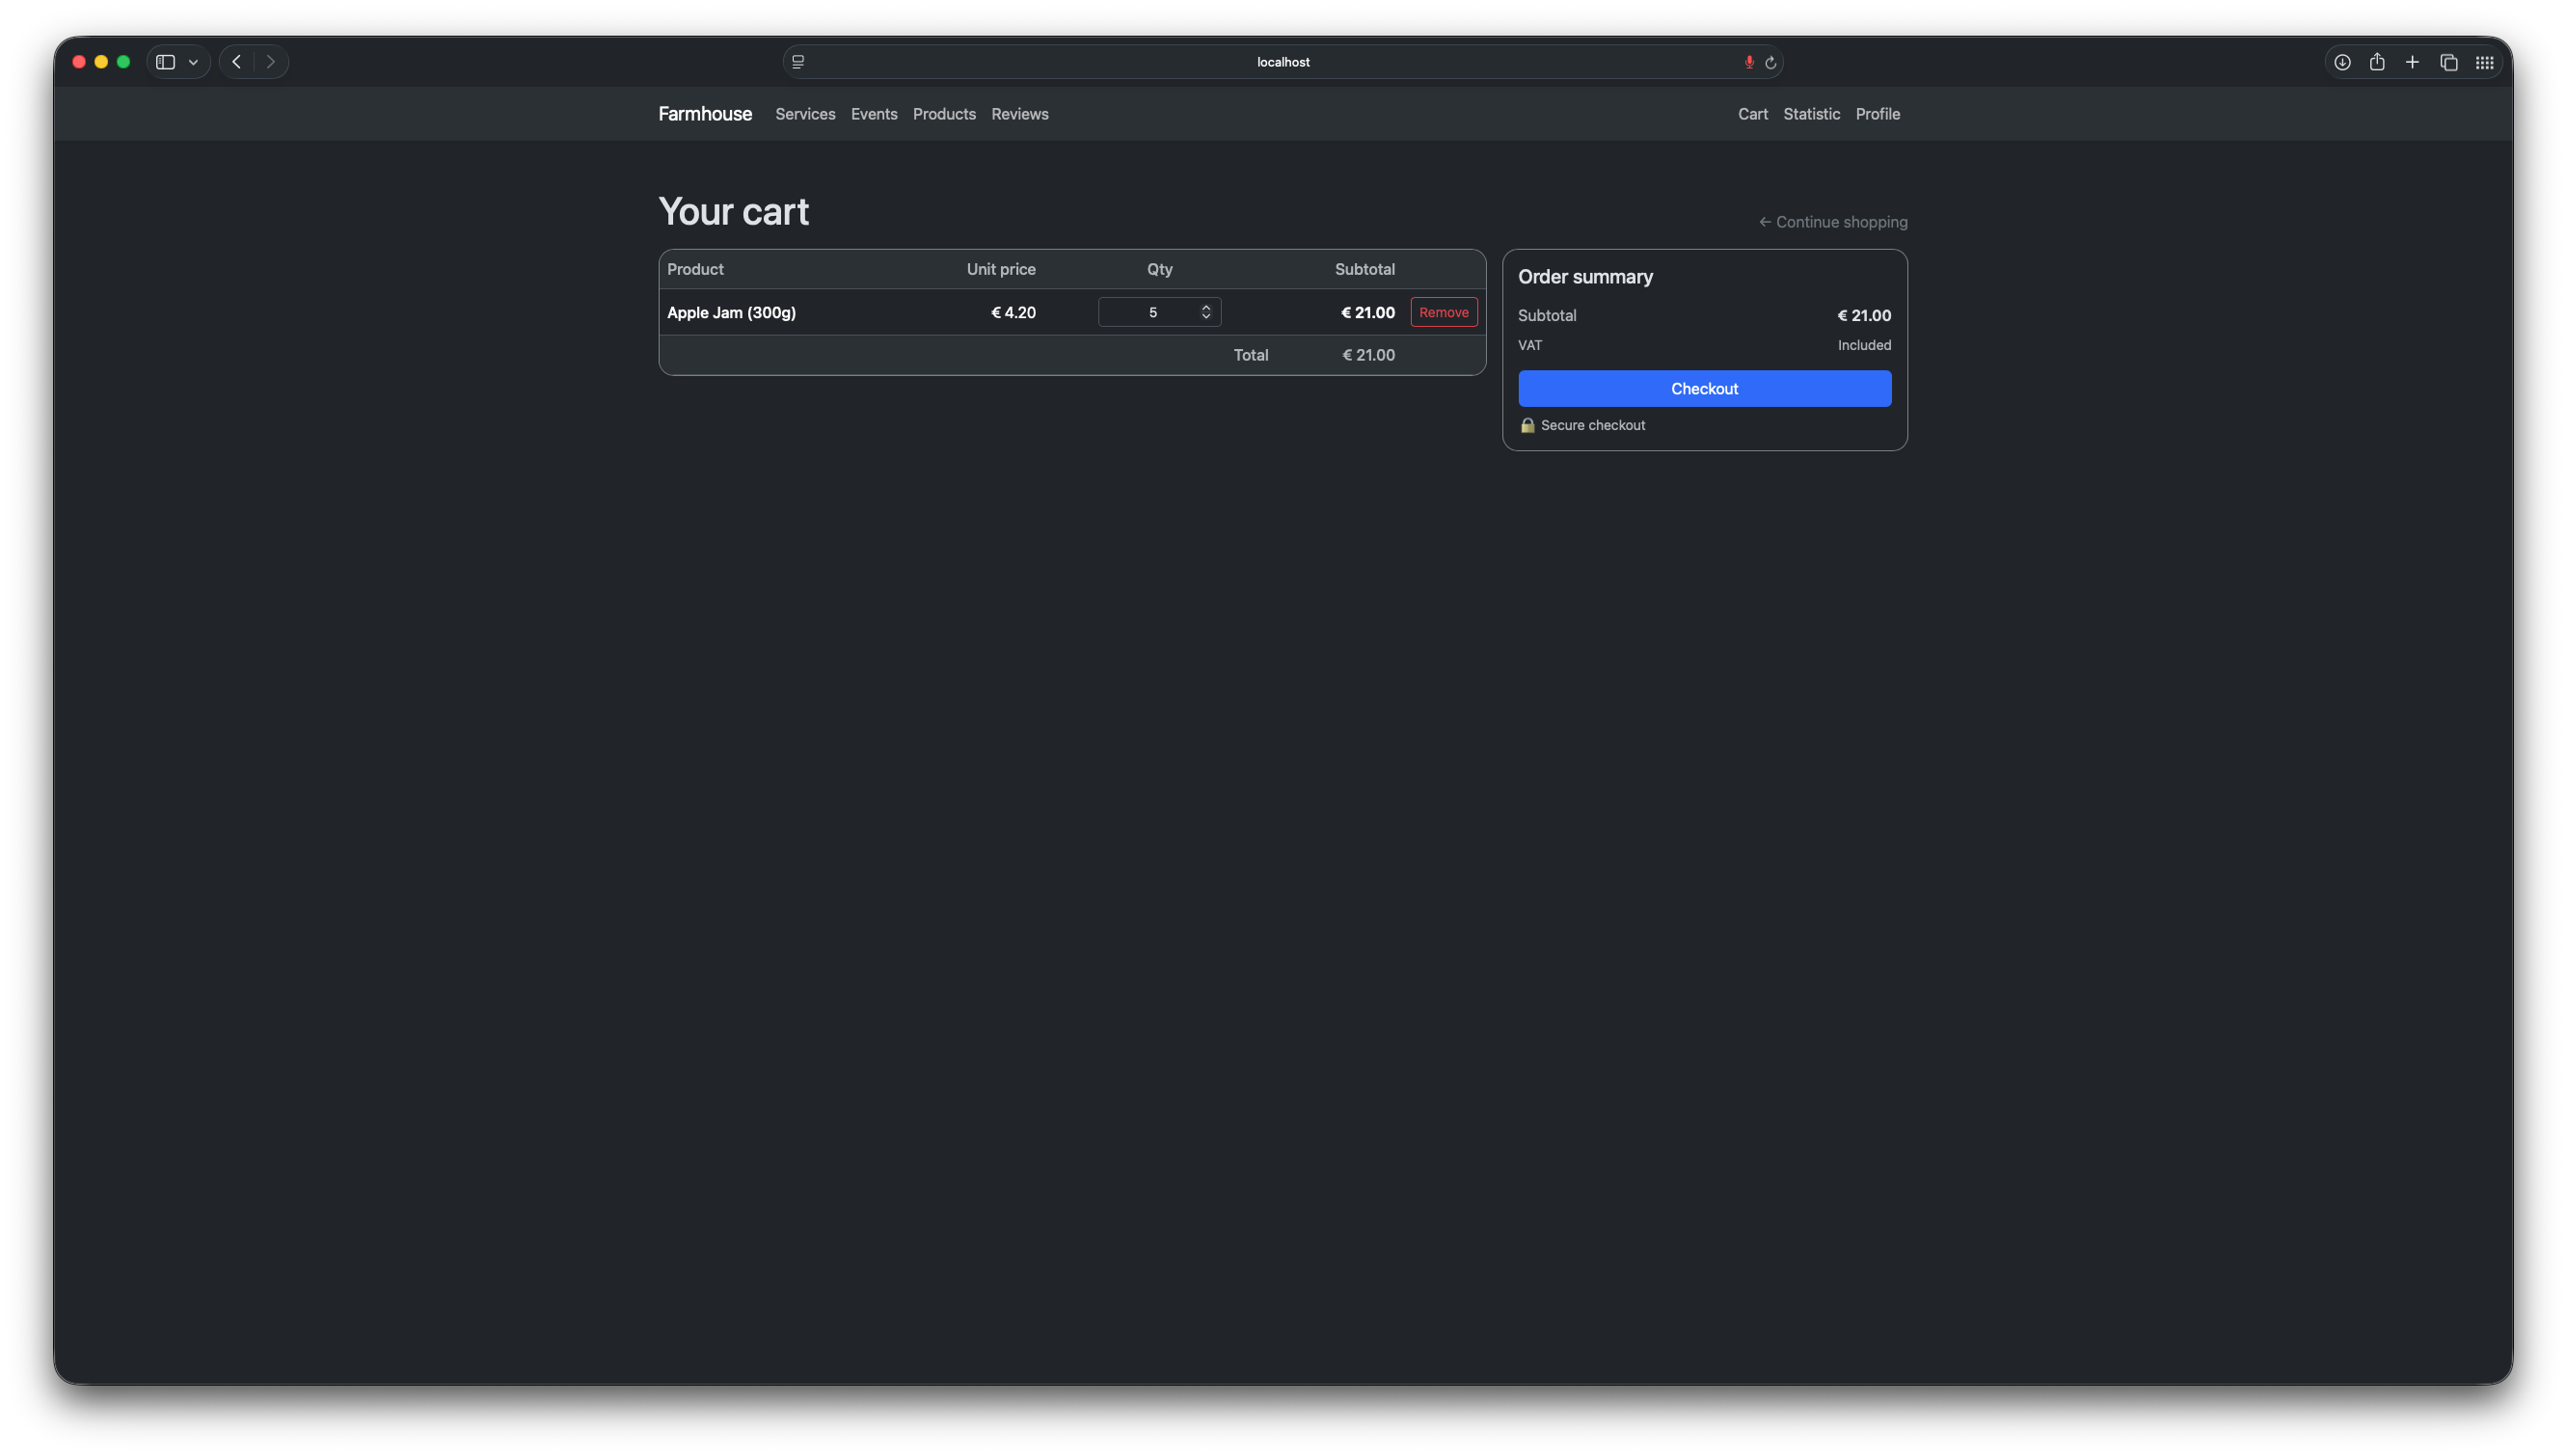
\includegraphics[width=\textwidth, trim=0 0 0 0]{./img/users/cart.png}
  \vspace{-1em}
  \label{fig:cart}
\end{figure}

\newpage
\section{Interfaccia Amministratore}
Per la gestione amministrativa, l'applicazione sfrutta la sezione
\textbf{Django Admin},
che consente agli amministratori di accedere rapidamente a tutte le
tabelle del database,
modificare dati, tramite un'interfaccia web sicura e strutturata.

\begin{figure}[H]
  \centering
  \includegraphics[width=\textwidth, trim=0 0 0 0]{./img/admin/djangoAdmin.png}
  \vspace{-1em}
  \label{fig:django-admin}
\end{figure}

Oltre al pannello standard di Django Admin, è stata realizzata una
pagina web dedicata alla
visualizzazione delle statistiche principali del sistema, come
l'andamento delle vendite, la
partecipazione agli eventi e la presenza del personale. Questa pagina
presenta tabelle
riepilogative.

\begin{figure}[H]
  \centering
  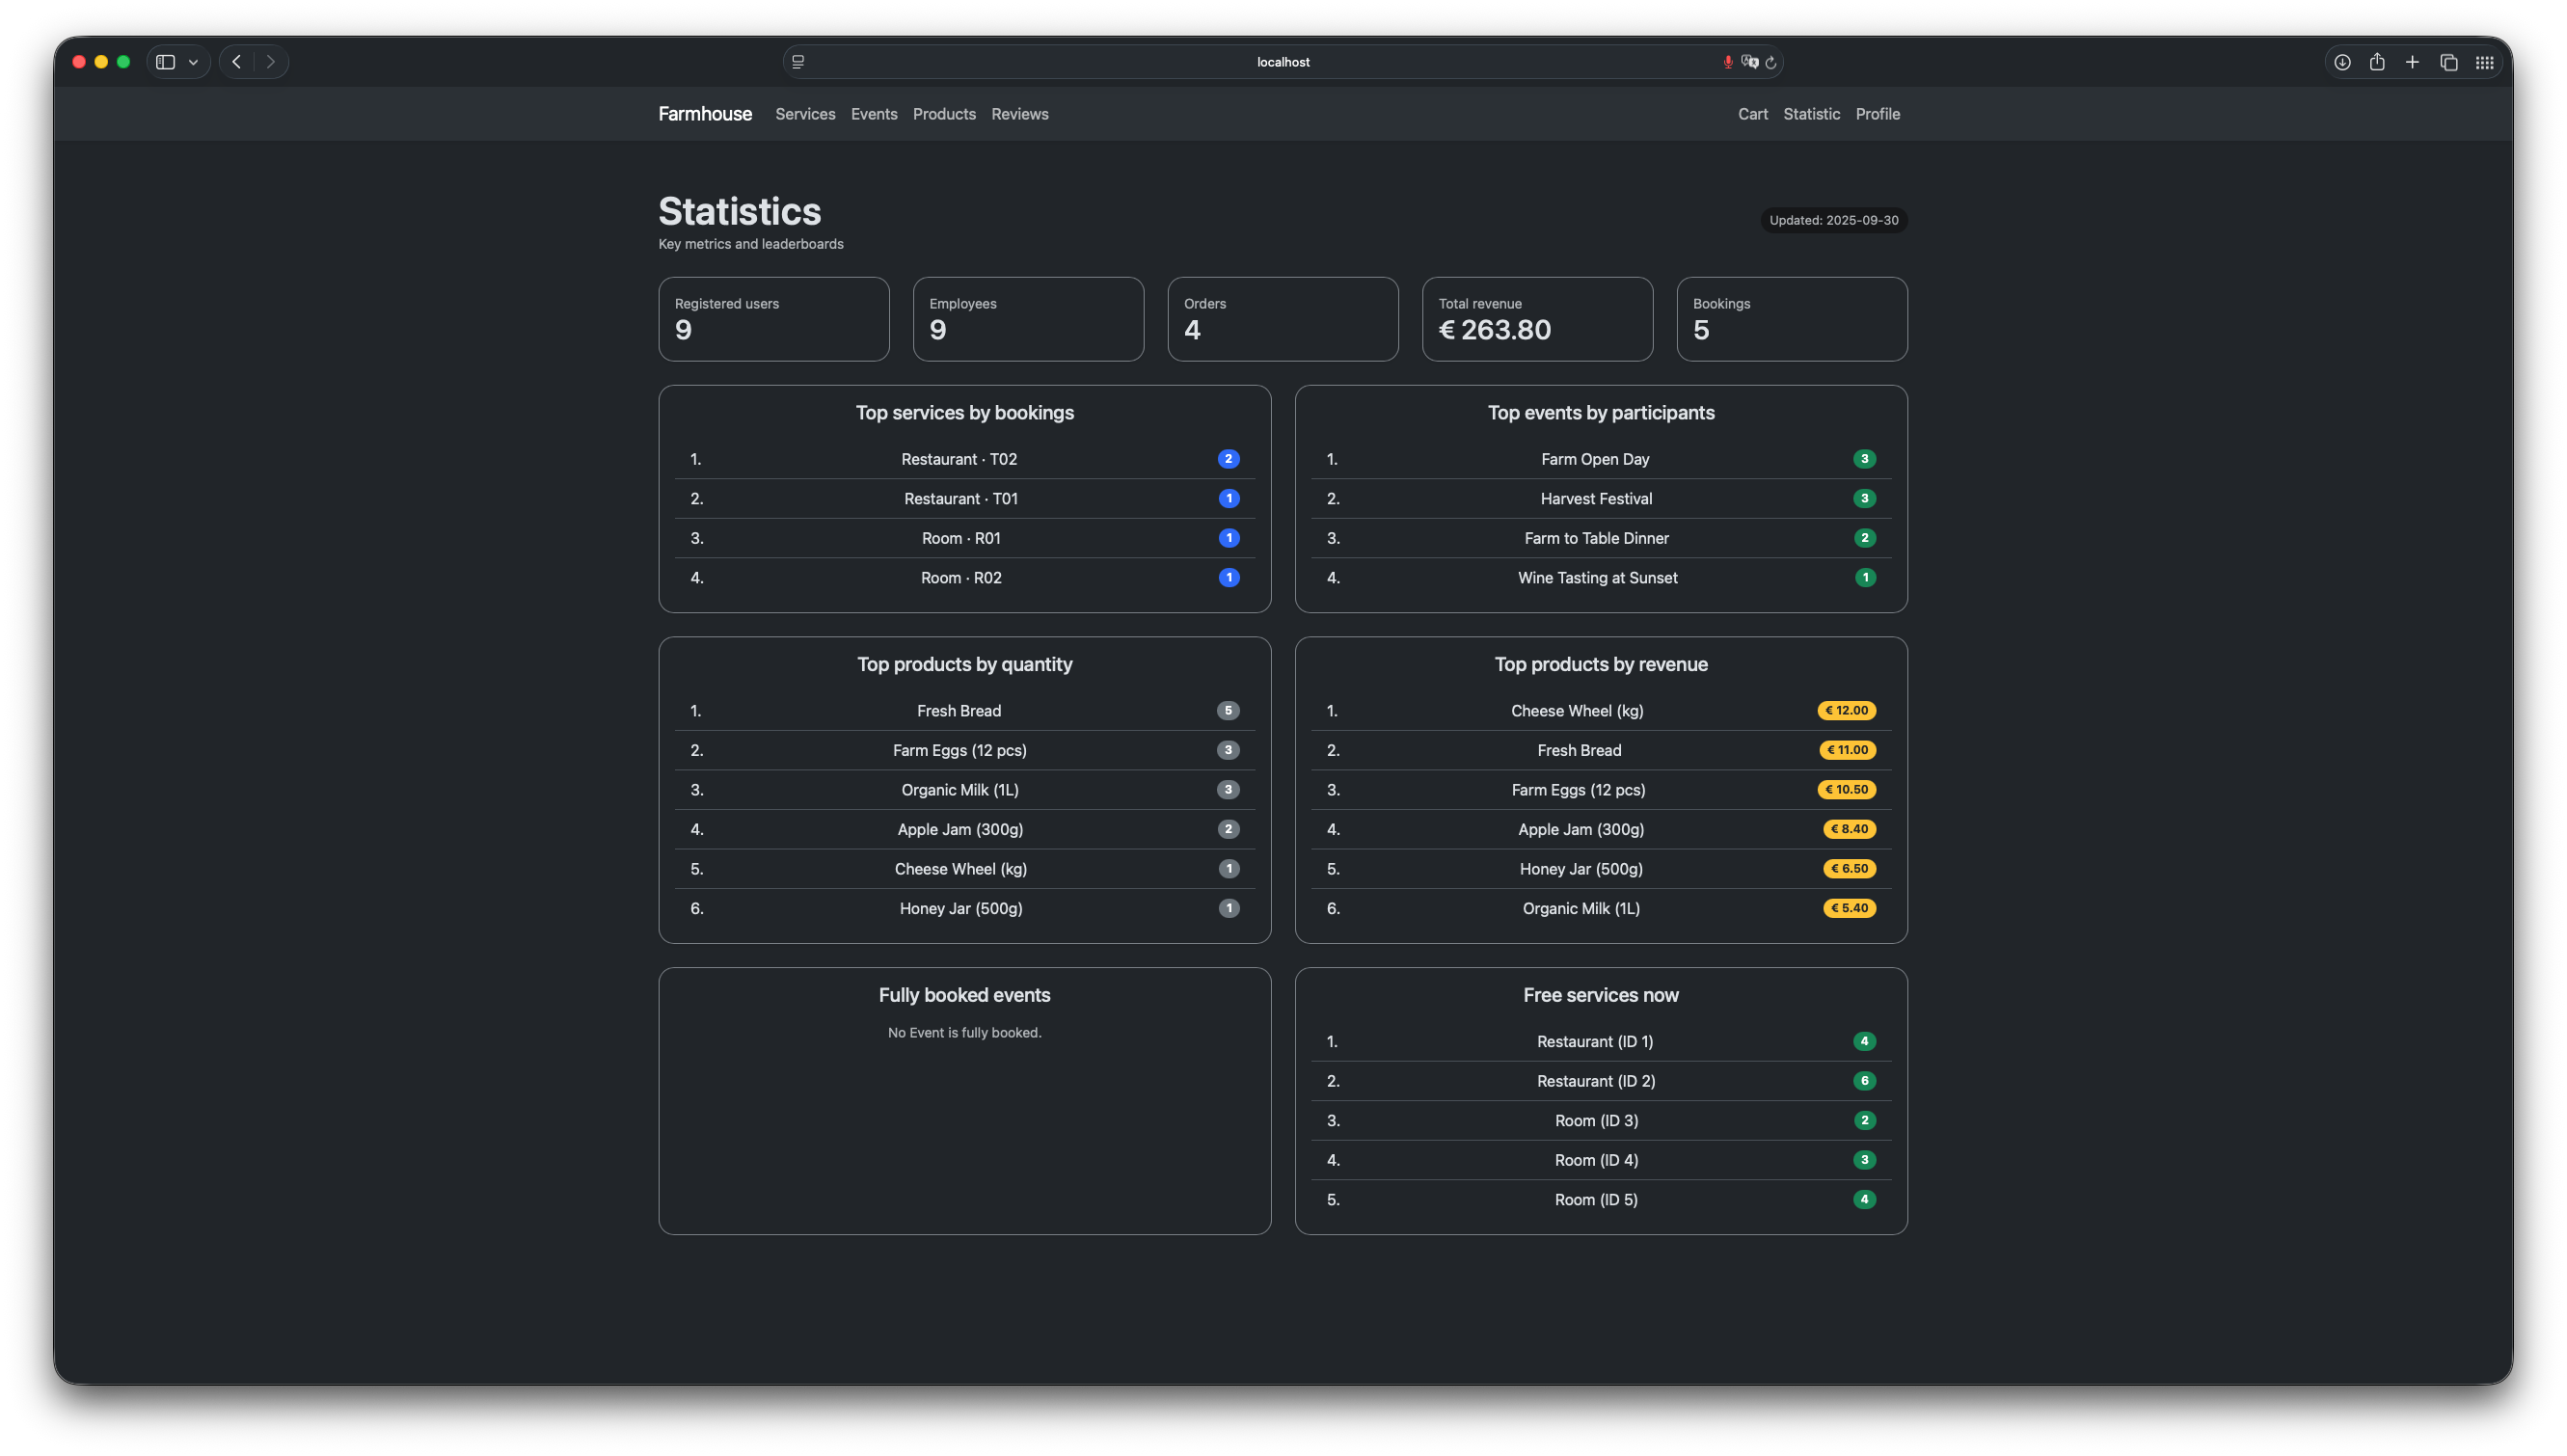
\includegraphics[width=\textwidth, trim=0 0 0 0]{./img/admin/statistic.png}
  \vspace{-1em}
  \label{fig:statistiche}
\end{figure}

\appendix
\chapter{Guida Utente}

\section{Clonazione del repository}
Clonare il progetto da GitHub e accedere alla cartella:

\begin{verbatim}
> git clone https://github.com/alessandrorebosio/D25-farmhouse.git
> cd DB25-farmhouse
\end{verbatim}

\section{Installazione delle dipendenze}

Si consiglia di utilizzare un ambiente virtuale Python per isolare le
dipendenze del progetto.

\begin{verbatim}
> python3 -m venv venv
\end{verbatim}

\noindent Attivazione dell'ambiente virtuale
\begin{verbatim}
# Su Linux/macOS:
> source venv/bin/activate
# Su Windows:
> venv\Scripts\activate
\end{verbatim}

\noindent Installazione delle dipendenze dal file requirements.txt
\begin{verbatim}
> pip install -r requirements.txt
\end{verbatim}

\section{Creazione del database}
Per creare il database MySQL a partire dagli script SQL forniti,
assicurarsi di avere MySQL
installato e in esecuzione.

\begin{verbatim}
> mysql -u root -p < app/sql/db.sql
> mysql -u root -p < app/sql/demo.sql
\end{verbatim}

Verrà richiesta la password dell'utente \texttt{root}. Il comando
eseguirà tutte le
istruzioni SQL contenute nel file \texttt{db.sql}, creando tabelle,
vincoli e dati di
esempio necessari per l'applicazione.

\section{Avvio dell'applicazione}

Per avviare l'applicazione Django, assicurarsi che l'ambiente
virtuale sia attivo e che il database
sia stato creato correttamente.

\begin{verbatim}
> python manage.py migrate
> python manage.py runserver
\end{verbatim}

L'applicazione sarà accessibile all'indirizzo
\url{http://localhost:8000/} tramite browser. Effettuare
il login o la registrazione per iniziare a utilizzare il sistema.

\end{document}
